\documentclass[10pt, twocolumn]{article}

\usepackage{report}

\usepackage[utf8]{inputenc} % allow utf-8 input
\usepackage[T1]{fontenc}    % use 8-bit T1 fonts
\usepackage[colorlinks=true, linkcolor=blue, citecolor=blue, urlcolor=blue]{hyperref}       % hyperlinks
\usepackage{url}            % simple URL typesetting
\usepackage{booktabs}       % professional-quality tables
\usepackage{amsfonts}       % blackboard math symbols
\usepackage{nicefrac}       % compact symbols for 1/2, etc.
\usepackage{microtype}      % microtypography
\usepackage{lipsum}		    
\usepackage{graphicx}
\usepackage{footnote}
\usepackage{doi}
\usepackage{comment}
\usepackage{multirow}
\usepackage{gensymb}
\usepackage{float}
\usepackage{amsmath}
\usepackage{subfig}
\usepackage[skip=10pt plus1pt, indent=30pt]{parskip}

\begin{document}

\begin{titlepage}
    \centering
    %
\includegraphics[width=2.3cm]{crest.jpg}\par
    \vspace{1cm}
    {\scshape\Large Department of Physics and Astronomy \par}
    \vspace{1cm}
    {\scshape\Large The University of Southampton \par}
    \vspace{1cm}
    \vspace{1cm}
    {\huge\bfseries The Forced Simple Pendulum \par}
    \vspace{1cm}
    {\Large Ong Chin Phin (Linus) \par}
    \vspace{1cm}
    {\Large Student ID: 33184747 \par}
    \vfill
    {\large November 2023 \par}
\end{titlepage}

%\maketitle
\newpage
\onecolumn
\tableofcontents
\thispagestyle{empty}
\clearpage

\newpage
\thispagestyle{empty}
\begin{abstract}
% Write what the experiment is about and what are the results 10-15 lines

%results go here
\end{abstract}

% keywords can be removed
%\keywords{First keyword \and Second keyword \and More}
\twocolumn
\newpage
\setcounter{page}{1}
\section{Introduction}
The forced simple pendulum looks, deceivingly simple. A bob on a string where the other end is attached to a fixed point is allowed to oscillate with an initial angular velocity and experiences a damping force with a frequency that acts against the pendulum - if the damping force (determined partly by a damping coefficient) is large enough, it will affect the motion of the oscillating pendulum. \\
\\
The equation of motion for a pendulum of a mass $m$ and length of $L$ is:
\begin{equation}
    mL^2 \frac{d^2\theta}{dt^2} + k \frac{d\theta}{dt} + mgL\sin({\theta}) = FL\cos({\Omega}t)
    \label{oscillation}
\end{equation}
Where:
\begin{itemize}
    \item $m$ is the mass of the pendulum bob
    \item $L$ is the length of the pendulum
    \item $\theta$ is the angular displacement of the pendulum from the vertical
    \item $\dot{\theta}$ is the angular velocity (rate of change of $\theta$)
    \item $\ddot{\theta}$ is the angular acceleration
    \item $k$ is the damping coefficient (dependent on the specific damping mechanism)
    \item $g$ is the acceleration due to gravity
    \item $F$ is the magnitude of the external force
    \item $\Omega$ is the frequency of the external force $F$
    \item $t$ is the time
    \item $k\dot{\theta}$ is the damping force
\end{itemize}
\\
\\
In the following sections, I introduce the method on how to change the 2nd order differential equation Eqn. (\ref{oscillation}) into a matrix equation in the form of $\vec{\bold{Y'}} = A\vec{\bold{Y}} - \vec{\bold{b}}$, such that they can be solved numerically using the Runge-Kutta method.
\\
\\
I will then investigate various scenarios, which will be introduced at the end of the Methodology section. Results are then compared to known data.
\\
\\
The Rayleigh-Lorentz pendulum \cite{Rayleigh1902}, named after Lord Rayleigh and Hendrik Lorentz, is a simple pendulum where the forcing frequency changes due to the change of the pendulum length
It has been shown that from \cite{Rayleigh1902}:
\begin{equation}
    \frac{E(t)}{f(t)} = \frac{E(0)}{f(0)}
    \label{adiabatic}
\end{equation}
Stating that the ratio of average energy to frequency is constant. This is an example of an adiabatic invariant - meaning that it is a conservation law that stays constant only when changes to the parameters are done slowly. The case of a uniform and exponential change in the pendulum length has been investigated in the case of a simple pendulum in \cite{Brearley1966, Werner1969, Ross1979} (for a uniform change) and \cite{SanchezZoido2013} (for both uniform and exponential), where the linear variation was determined by the equation $l(t) = l_0 (1 + \epsilon{t})$, and the exponentially varying case is given by the equation $l(t) = l_0\exp{\epsilon t}$. Where $\epsilon$ in both equations is a small parameter of unit $s^{-1}$. There are many other variations that I can investigate, for example, a non-linear (quadratic or higher order) variation, or even a random variation (Brownian motion or random walks). A random walk is an interesting option for several reasons:
\begin{itemize}
    \item Real-world systems are experiencing random fluctuations. For example, a skyscraper or bridge will not experience a constant force.
    \item Stability of the pendulum system could be assessed. What is the optimum pendulum (one that is resilient to random changes in forces)?
    \item Resonant frequencies can be identified easily
    \item Long term behaviour prediction
\end{itemize}
\section{Methodology}
Since time is measured relative to the period of free oscillations of small amplitude, I can write:
\begin{equation}
    t = \tau\sqrt{\frac{L}{g}}
    \label{modified time}
\end{equation}
And:
\begin{equation}
    \Omega = (1 - \eta)\sqrt{\frac{g}{L}}
    \label{modified omega}
\end{equation}
To investigate the situation where the behaviour of the pendulum when the forcing frequency, $\Omega$ is slightly less than the natural frequency, $\frac{g}{L}$.
To convert equation (\ref{oscillation}) into dimensionless form, we recall that: $t = \tau\sqrt{\frac{L}{g}}$  and by the chain rule, $\frac{d\tau}{dt} = \frac{d\theta}{dt}\frac{dt}{d\tau}$ give the following equations:
\begin{equation}
    \begin{split}
        \frac{d\theta}{dt} = \sqrt{\frac{g}{L}}\frac{d\theta}{d\tau} \\
        \frac{d^2\theta}{dt^2} = \frac{g}{L}\frac{d^2\theta}{d\tau^2}
    \end{split}
    \label{chain rules}
\end{equation}
Which can be substituted into equation (\ref{oscillation}) after dividing by $mgL$ and substituting equation (\ref{modified time}) and (\ref{modified omega}).
\begin{equation}
        \centering
        \begin{split}
            & (\frac{L}{g})(\frac{g}{L})\frac{d^2\theta}{d\tau^2} + \frac{k}{mgL}\sqrt{\frac{g}{L}}\frac{d\theta}{d\tau} + \sin(\theta)\\
            & = \frac{F}{mg}\cos((1 - \eta)\sqrt{\frac{g}{L}}\sqrt{\frac{L}{g}}\tau)
        \end{split}    
\end{equation}
The dimensionless form of equation (\ref{oscillation}) is then:
\begin{equation}
    \frac{d^2\theta}{d\tau^2} = -\alpha\frac{d\theta}{d\tau} - \sin(\theta) + \beta\cos((1 - \eta)\tau)
    \label{dimensionless}
\end{equation}
With parameters\footnote{
    Note that:
    \\
        \begin{equation}
            \frac{k}{mgL}\sqrt{\frac{g}{L}} = \frac{k}{mL\sqrt{g}\cdot\sqrt{g}}\sqrt{\frac{g}{L}} = \frac{k}{mL\sqrt{gL}}
        \end{equation}
}: 
\begin{equation}
    \centering
    \begin{split}
        \alpha &= \frac{k}{mL\sqrt{gL}}\\
        \beta &= \frac{F}{mg}
    \end{split}
    \label{parameters}
\end{equation}
The RK4(5) (Runge–Kutta–Fehlberg) method will be used to solve the equation numerically. I will be using \verb|scipy.integrate.RK45| that uses the Dormand-Prince pair of formulas \cite{DormandPrince1980}. To solve a 2nd-order differential equation with any Runge-Kutta method, the ODE in question will have to be expressed as a 1st-order ODE. 
From equation (\ref{dimensionless}) and taking the substitution:
\begin{equation}
    \omega = \frac{d\theta}{d\tau}
\end{equation}
The ODE will be a system of equations of the form $\vec{\bold{Y'}} = A\vec{\bold{Y}} - \vec{\bold{b}}$.
\begin{gather} \label{matrixform}
    \begin{bmatrix}
        \theta' \\ 
        \omega'
    \end{bmatrix}
    =
    \begin{bmatrix}
        0 & 1 \\
        $-\sin(\theta)$ & $-\alpha$
    \end{bmatrix}
    \begin{bmatrix}
        \theta \\ 
        \omega
    \end{bmatrix}
    -
    \begin{bmatrix}
        0 \\
        $\beta\cos((1 - \eta)\tau)$        
    \end{bmatrix}
\end{gather}
For the Rayleigh-Lorentz (R-L) pendulum, the R.H.S. term in Equation \eqref{oscillation} can now be simplified to $FL$, because now $L$ will be a random number (which emerges from the random walk). The forcing frequency is now determined by the changes in L. The matrix equation that follows is a simplified version of Eqn. \eqref{matrixform}.
\begin{gather} \label{RLmatrixform}
    \begin{bmatrix}
        \theta' \\ 
        \omega'
    \end{bmatrix}
    =
    \begin{bmatrix}
        0 & 1 \\
        $-\sin(\theta)$ & $-\alpha$
    \end{bmatrix}
    \begin{bmatrix}
        \theta \\ 
        \omega
    \end{bmatrix}
    -
    \begin{bmatrix}
        0 \\
        $\beta$        
    \end{bmatrix}
\end{gather}
The distribution for the random walk for $L$ will be a normal distribution using \verb|numpy.random.Generator.normal|\footnote{Documentation can be found \href{https://numpy.org/doc/stable/reference/random/generated/numpy.random.Generator.normal.html}{here}}. The reason for using a normal distribution is that normal distributions are prevalent, and on an experiment regarding forces on a pendulum, I think it makes sense to have a real-world lens on how a forced pendulum behaves \cite{Peebles2001}.

\section{Setup}\label{setup}
The code used for the entirety of the project can be found on my \href{https://github.com/linsuong/PHYS-6017-Labs/blob/main/Projects/ForcedSimplePendulum}{GitHub page}. 
\\
\\
First, I think it is useful to have a rough understanding of the effects of each parameter on the numerical solution of the pendulum. By assigning values to the constants and iterating each one, I can (without complete certainty, of course) predict the pendulum behaviour for later experiments.
The system is set up as follows:
\begin{itemize}
    \item The pendulum has a mass $m$ of 1kg
    \item The length of the string, $L$ is 2 meters
    \item The damping coefficient $k$ has a value of 0.5
    \item The factor $\eta$ has a value of 0.1
    \item The magnitude of the force $F$ is 10N
    \item $g$ is 9.81$ms^{-1}$
    \item Time interval is 0 to 50 seconds \footnote{As the RK4(5) algorithm goes for longer, the errors stack up. It is not wise to use a long time interval at once without taking any precautions. Therefore a relatively short integration time period is investigated.}
\end{itemize}
By modifying each parameter, I plot the time-domain ($\theta$ against $t$) and the phase portrait\footnote{See Section \ref{phase plots appendix} for an explanation on phase portraits, as this is not covered in any core module.}  in Figs. (\ref{time domain test} and \ref{phase portrait test}). Each notable simulation will contain a time-domain plot and a phase portrait plot ($\frac{d\theta}{dt}$ against $\theta$). \\
\\
I noticed an interesting pattern as the mass changes. As the mass of the pendulum bob increased, the motion of the pendulum went from a simple harmonic to a dampened system. This is probably because the magnitude of the external force was not enough to keep the pendulum in a simple harmonic motion. As the force was modified, what changed was just the magnitude of oscillation of the pendulum, up to as high as 30 radians. This meant that the pendulum would have completed many full rotations ($\sim{9}$ for $\theta\sim{30}$).Increasing the length allowed the pendulum to do complete rotations in some cases. An increase in length meant an increase in angular velocity. A change in length should also affect the frequency\footnote{Recall $f = \frac{1}{2\pi}\frac{g}{L}$}, as a longer pendulum length will result in a shorter frequency (longer time to complete one oscillation). 

\onecolumn
\begin{figure}
    \centering
    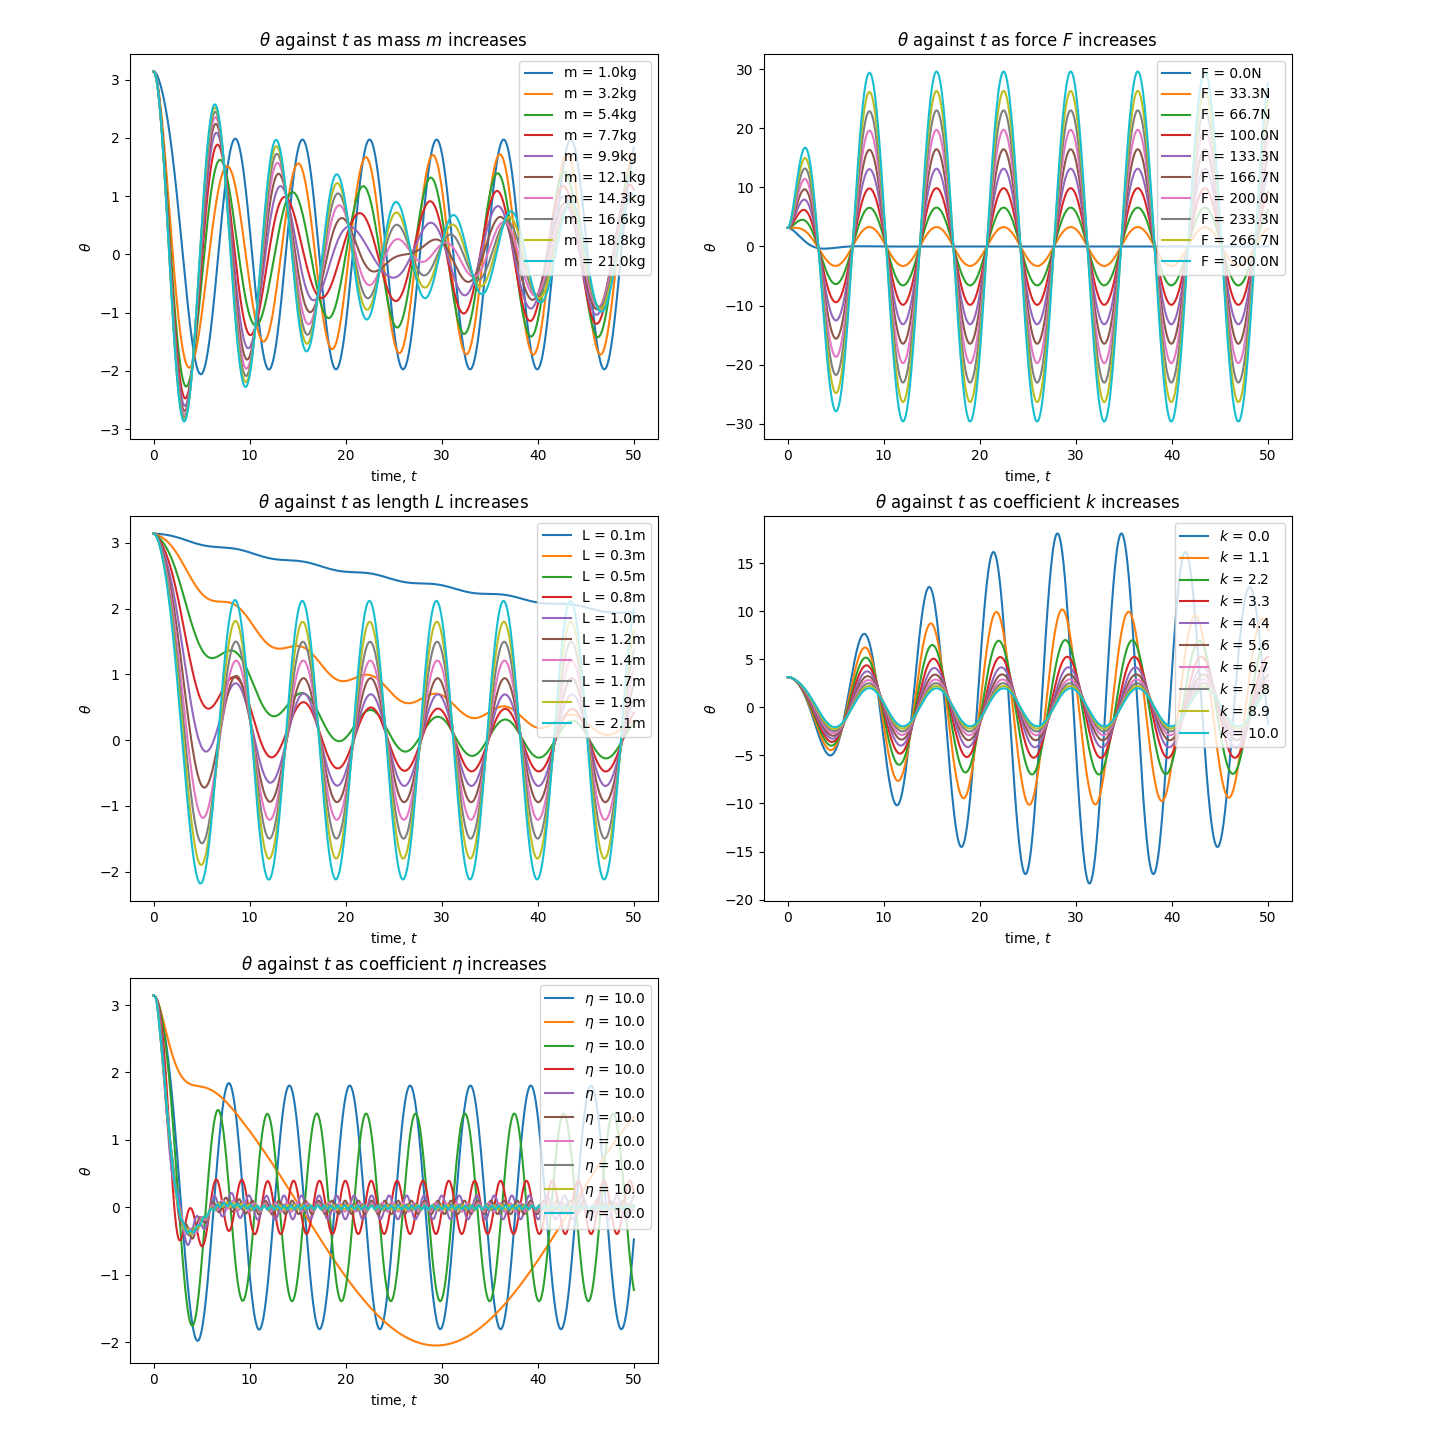
\includegraphics[width = 1.2\columnwidth]{Projects/ForcedSimplePendulum/Plots/test_plots.png}
    \caption{Time-domain plots for the case of the simple forced pendulum, where each variable is iterated one by one.}
    \label{time domain test}
\end{figure}

\begin{figure}
    \centering
    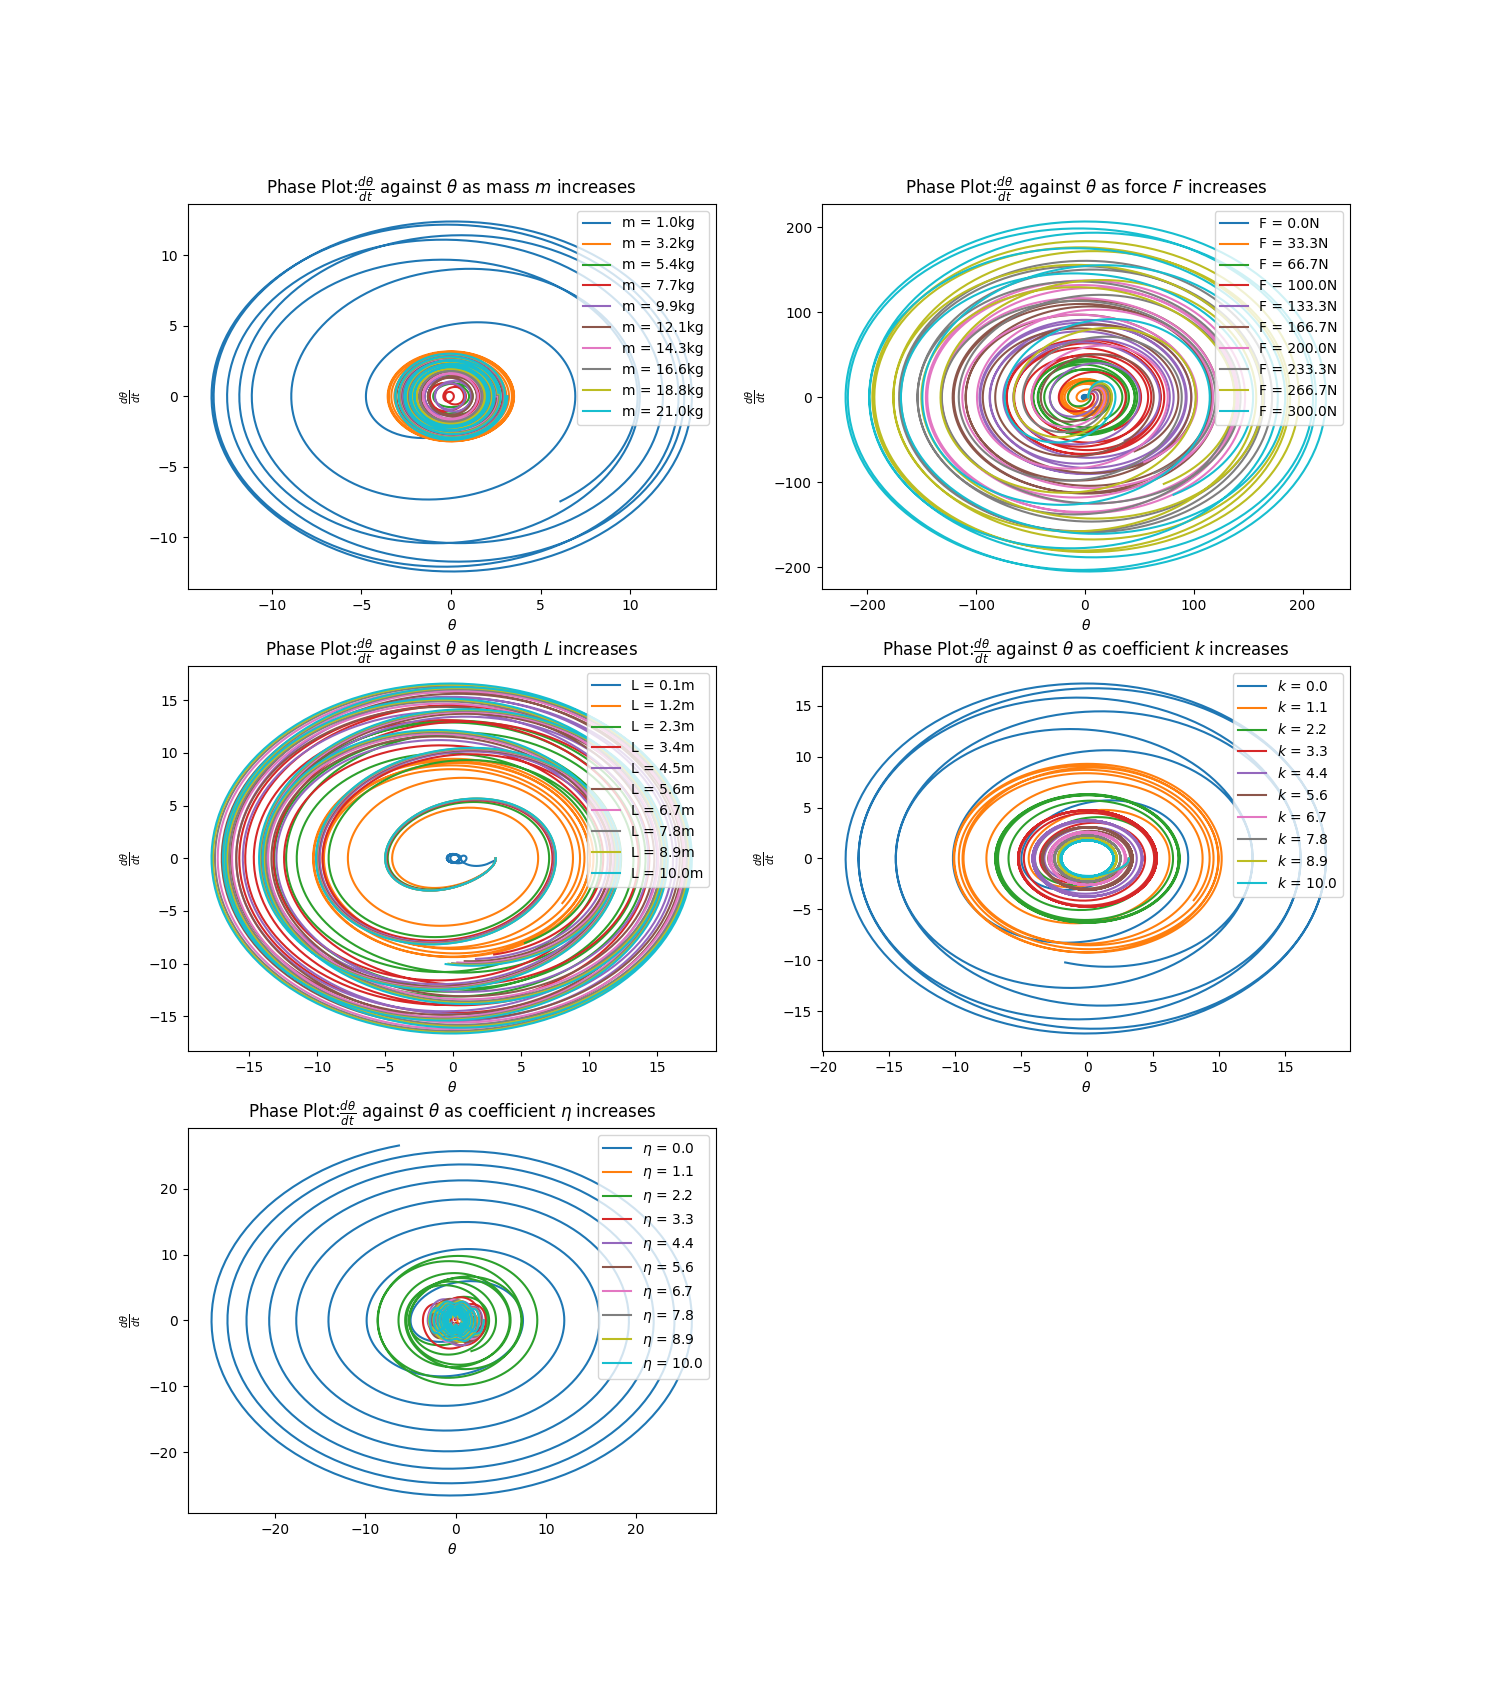
\includegraphics[width = 1.2\columnwidth]{Projects/ForcedSimplePendulum/Plots/test_plots_phase.png}
    \caption{Phase portraits for the case of the simple forced pendulum, where each variable is iterated one by one.}
    \label{phase portrait test}
\end{figure}

\twocolumn
\section{Areas of Investigation}
For the simple forced pendulum, I will investigate the case when the external force, $F$ is almost equal to $mg$ -- $F \sim{mg}$. I iterate through values of $k$, decreasing $k$ until something happens. With the same values of the other constants in Section \ref{setup}, with the exception of $F = 10N$ and iterating over values of $k$ until something happens.\\
\\
For the R-L pendulum, I will implement the case where the length of the pendulum changes with a random walk, and verify if Equation \eqref{adiabatic} still holds for the case of a random walk. The energies in this system are simply the kinetic and potential energy, given by:
\begin{equation}
    T = \frac{1}{2}mv^2 = \frac{1}{2}m(L\omega)^2
\end{equation}
\begin{equation}
    V = mgL\cos(\theta) 
\end{equation}
The angular frequency at each time step can be calculated by
\begin{equation}
    \omega = 2\pi{f} = \sqrt{\frac{g}{L}}
\end{equation}
The algorithm will run for several iterations, and then an average of the angular displacement, angular velocity, length of pendulum, frequency and energy will be taken at every time step. 4 important graphs will be plotted: the time-domain plot, phase domain plot, plot of average values of L against t, and the difference of the average energy-frequency ratio at $t = 0$ to the values of energy-frequency at each time step.
\section{Results}
\subsection{$F \sim{mg}$}
By iterating through different values of $k$, the following time-domain and phase plots are obtained (when something interesting happened - the not-so-interesting plots can be found in Section \ref{plotsFmg}. I won't bore you with 20 different-but-not-too-different plots). After testing different ranges of $k$, I found a range where something interesting happened.
\onecolumn
\begin{figure}
    \centering
    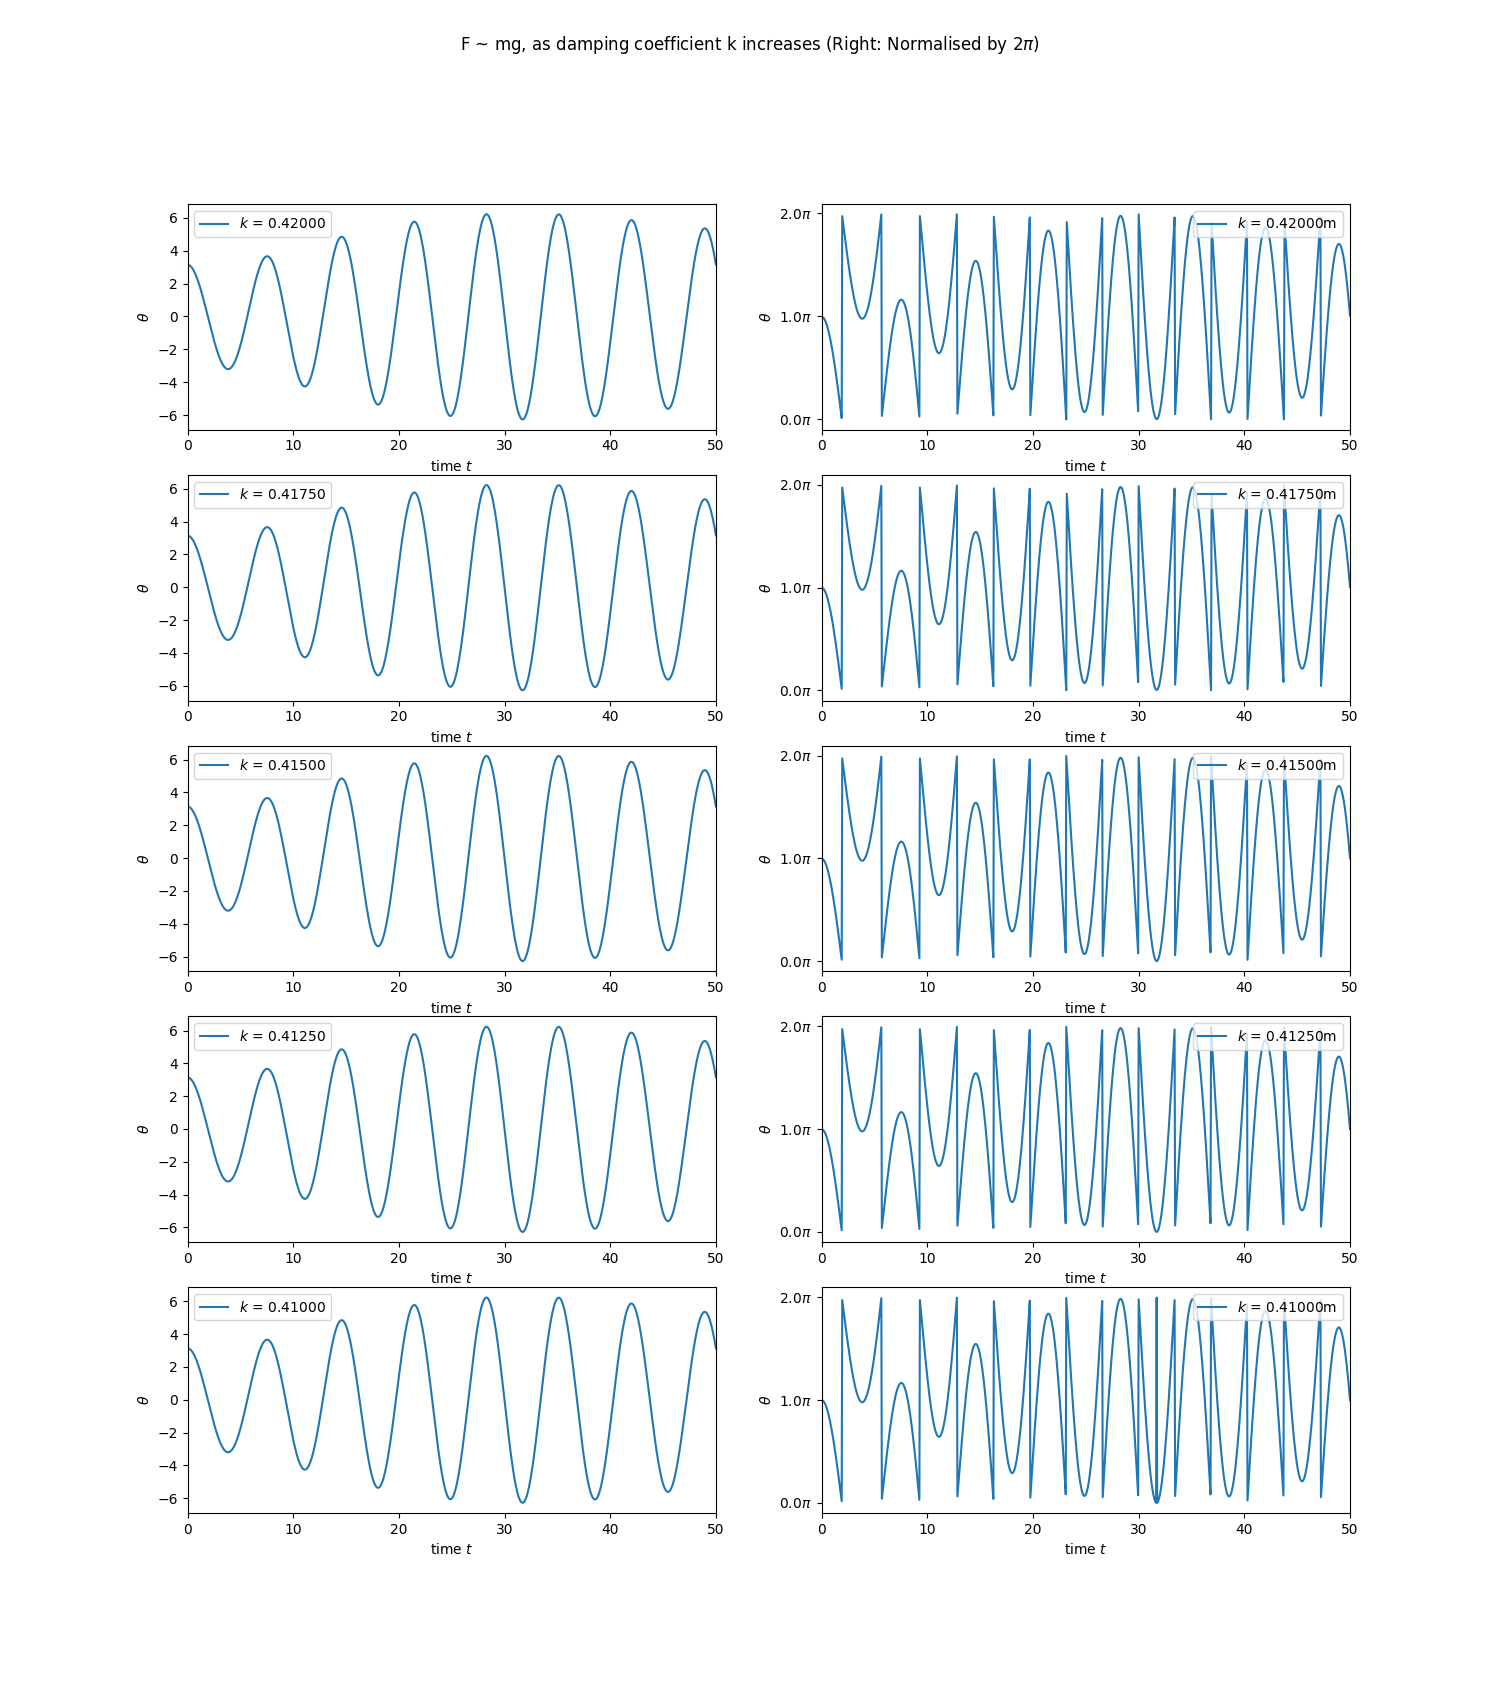
\includegraphics[width= \columnwidth]{Projects/ForcedSimplePendulum/Plots/F~mg as damping coefficient k increases from 0.42 to 0.41.png}
    \caption{Time-domain plot for the forced simple pendulum for the case of $F \sim{mg}$ for $k = 0.42$ to $k = 0.41$. (Left column: raw data; Right column: data normalised by $2\pi$)}
    \label{k 5 to 1 short}
\end{figure}
\twocolumn
At $k = 0.41$,
\begin{figure}[H]
    \centering
    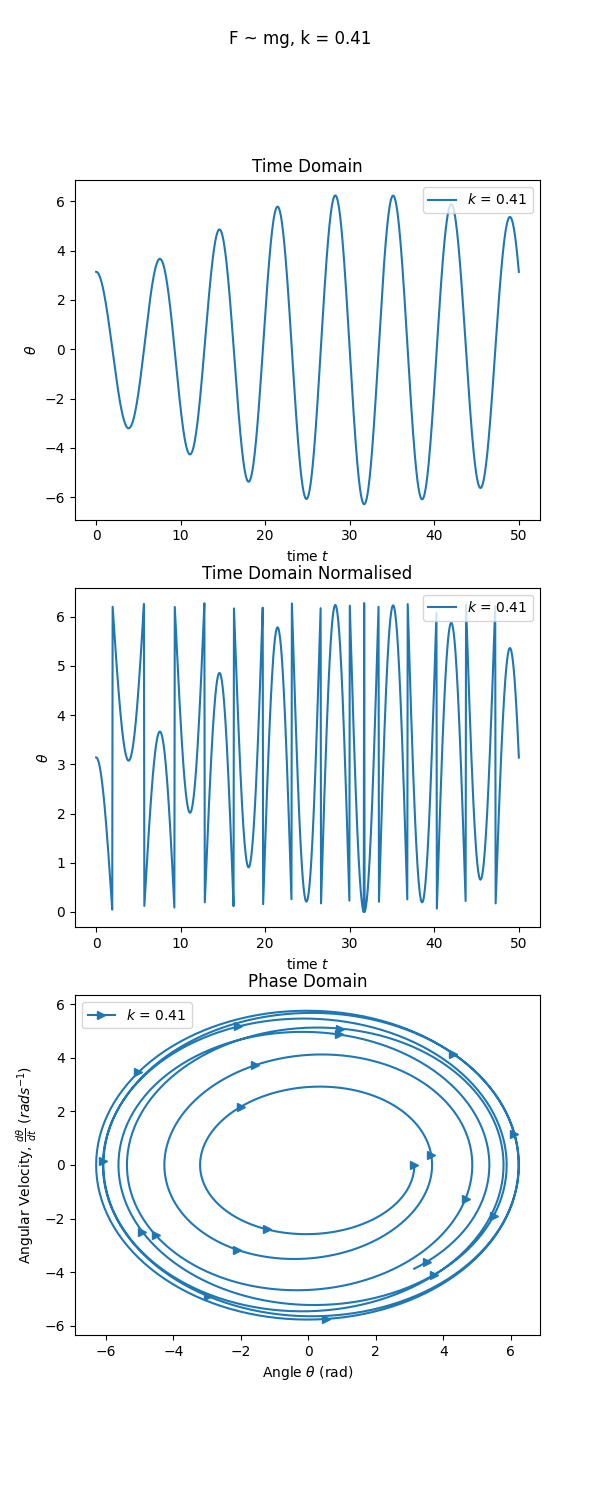
\includegraphics[width = 0.9\columnwidth]{Projects/ForcedSimplePendulum/Plots/Plot of F~mg, k is 0.41.png}
    \caption{Plots for the case of $F\sim{mg}$ when $k = 0.41$. Animation \href{https://github.com/linsuong/PHYS-6017-Labs/blob/main/Projects/ForcedSimplePendulum/Plots/F~mg\%2C\%20k\%20is\%200.41.gif}{here}.}
    \label{k = 0.41}
\end{figure}
I also investigated the case of a longer period but found nothing of interest (Fig. \ref{k = 0.41 med} and \ref{k = 0.41 long}). The significance and physical meaning will be discussed further in Section \ref{analysisFmg}.
\subsection{Rayleigh-Lorentz Pendulum Random Walk}{\label{rlresults}}
The bottom left and right plots are the emphasis of this section of the project. Therefore I will only show the time-domain and phase-domain plots for the first iteration. The more complete plots can be found in Section \ref{rlplots}
\begin{figure}
    \centering
    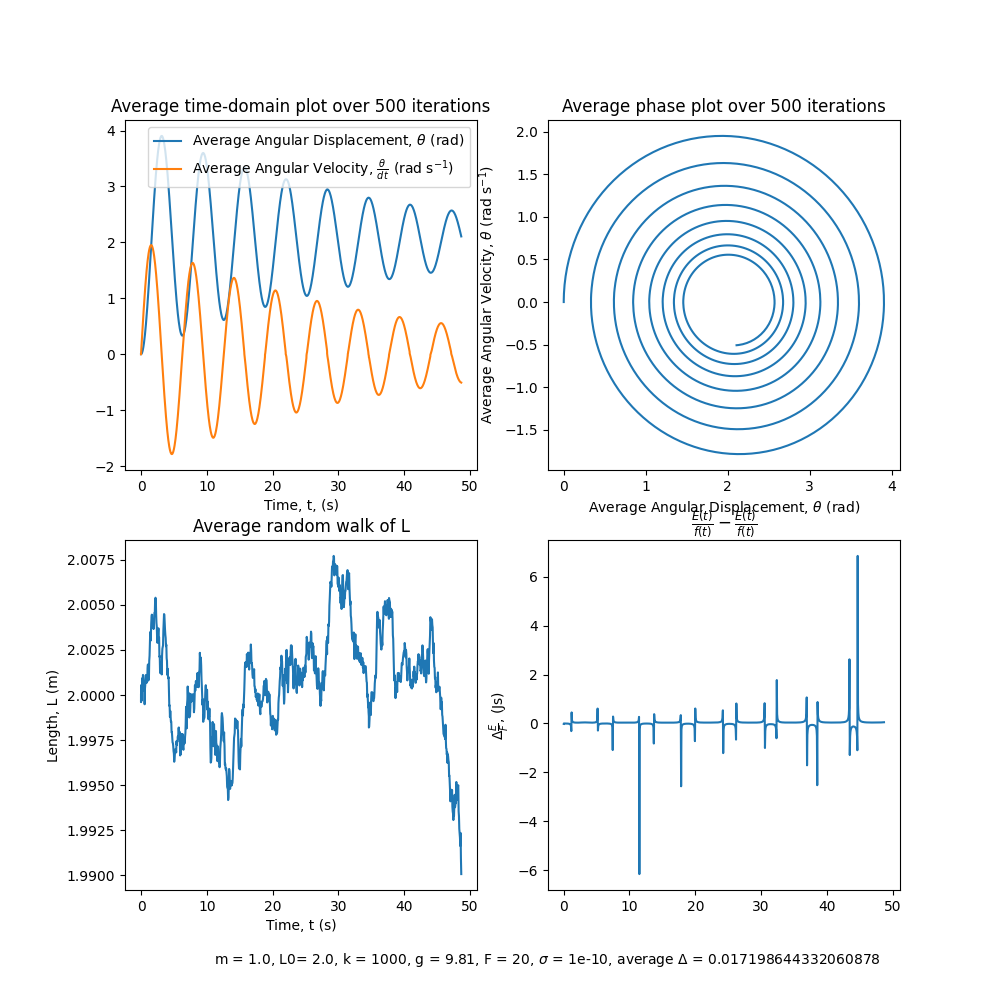
\includegraphics[width = \columnwidth]{Projects/ForcedSimplePendulum/Plots/m = 1.0, L0= 2.0, k = 1000, g = 9.81, F = 20, sigma = 1e-10, run number 0.png}
    \caption{First Iteration.}
    \label{fig:enter-label}
\end{figure}

\begin{figure}
    \centering
    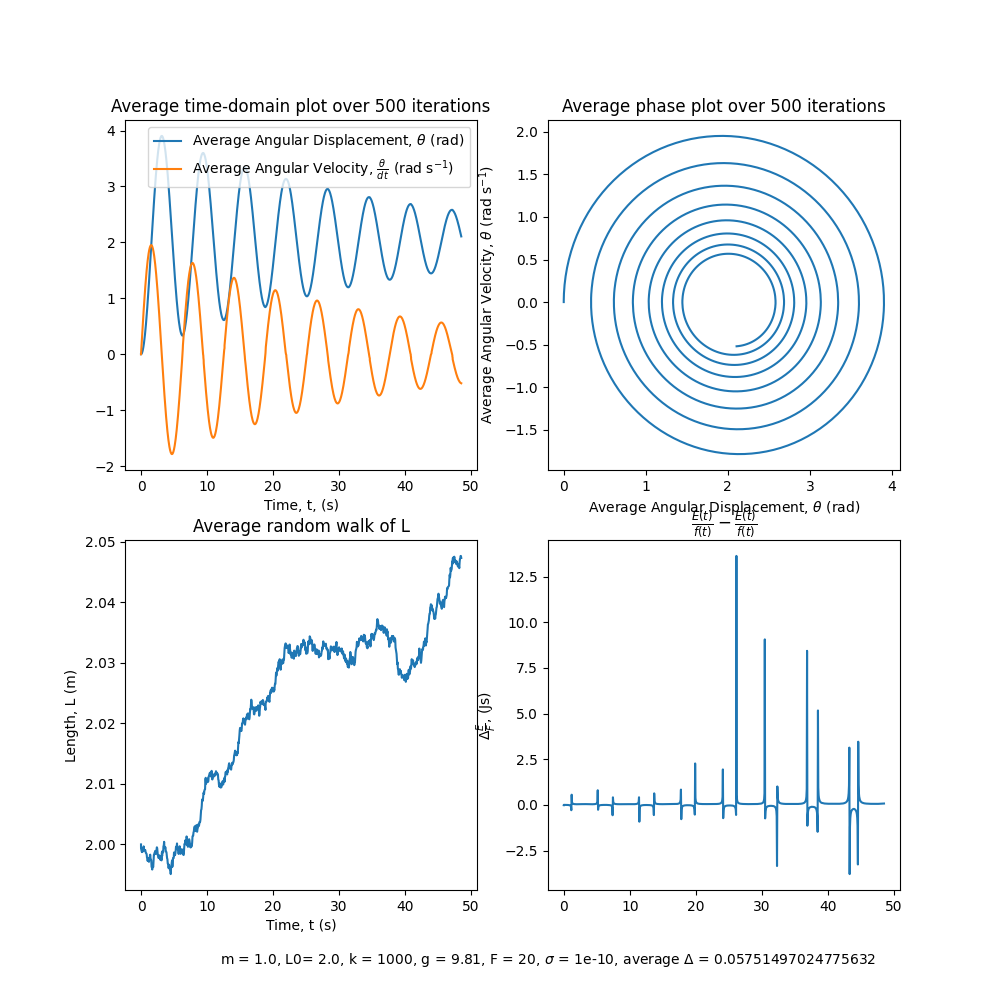
\includegraphics[width = \columnwidth]{Projects/ForcedSimplePendulum/Plots/m = 1.0, L0= 2.0, k = 1000, g = 9.81, F = 20, sigma = 1e-10, run number 1.png}
    \caption{Second Iteration.}
    \label{fig:enter-label}
\end{figure}

\begin{figure}
    \centering
    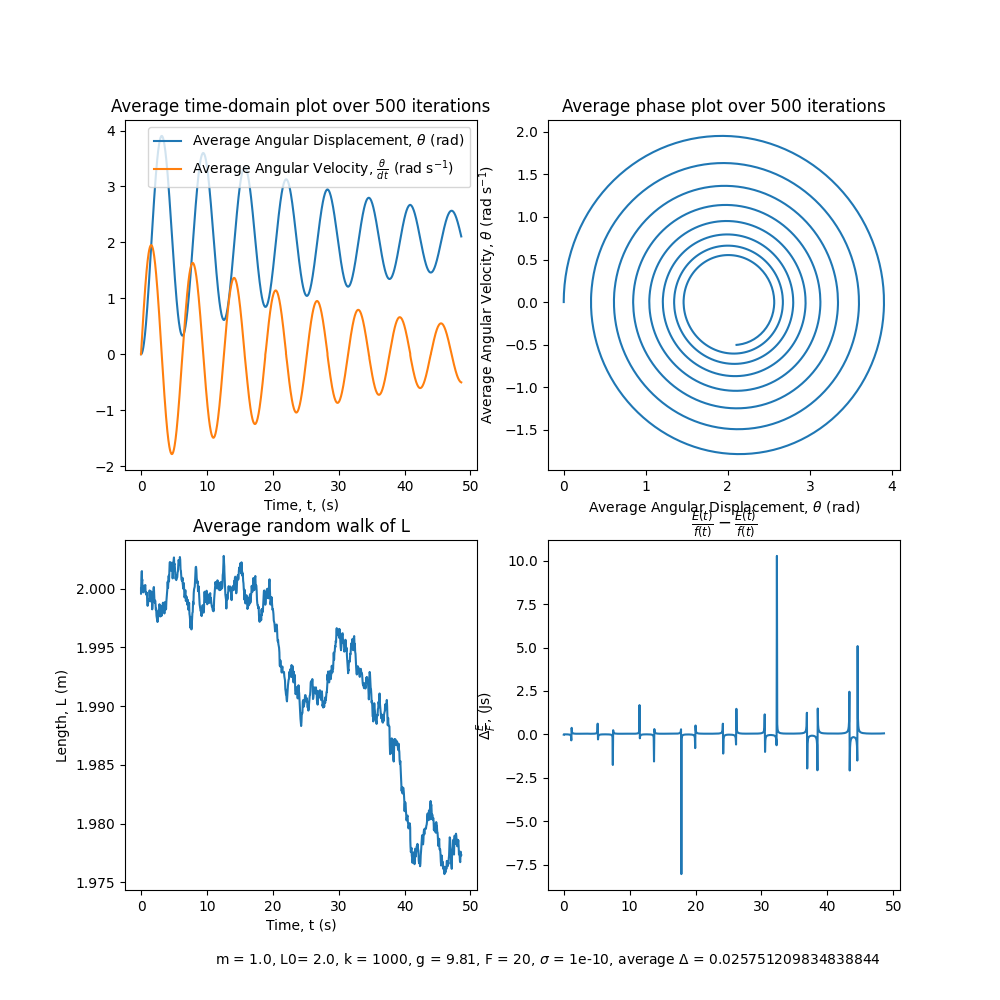
\includegraphics[width = \columnwidth]{Projects/ForcedSimplePendulum/Plots/m = 1.0, L0= 2.0, k = 1000, g = 9.81, F = 20, sigma = 1e-10, run number 2.png}
    \caption{Third Iteration.}
    \label{fig:enter-label}
\end{figure}

\begin{figure}
    \centering
    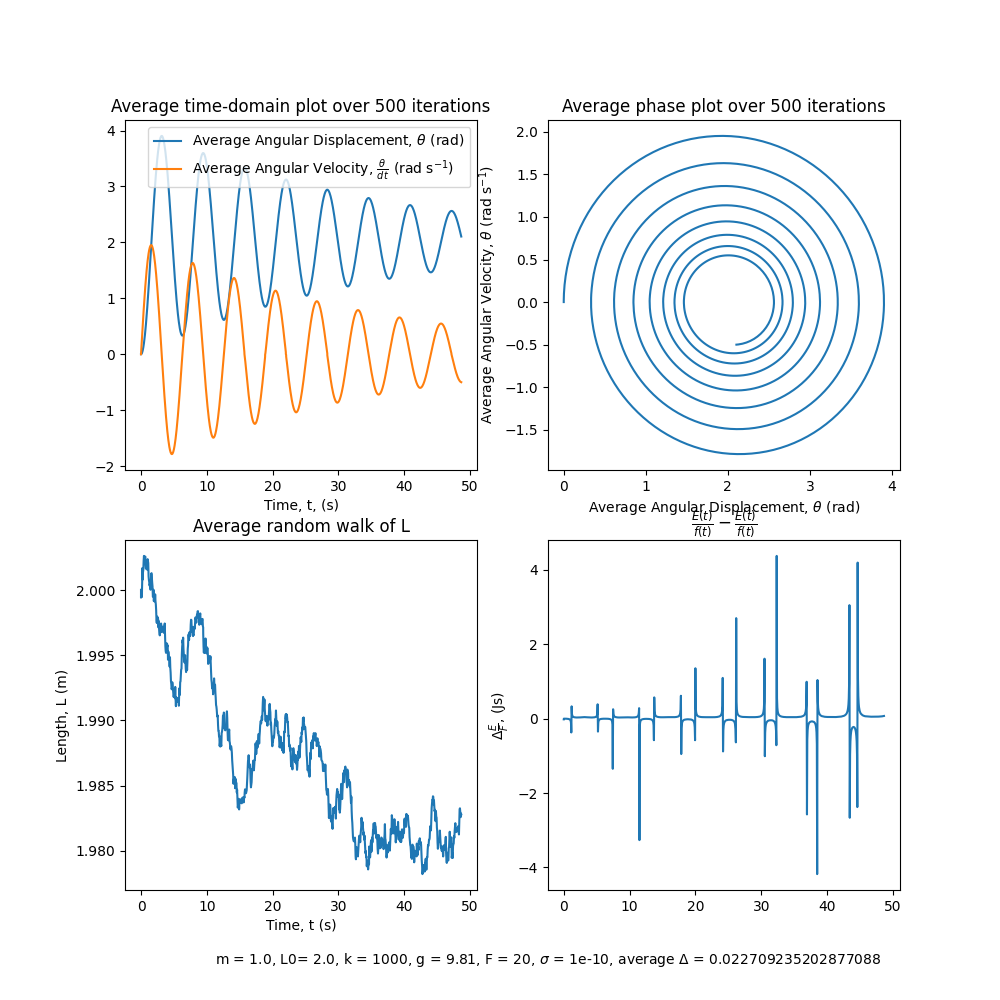
\includegraphics[width = \columnwidth]{Projects/ForcedSimplePendulum/Plots/m = 1.0, L0= 2.0, k = 1000, g = 9.81, F = 20, sigma = 1e-10, run number 3.png}
    \caption{Fourth Iteration.}
    \label{fig:enter-label}
\end{figure}

\begin{figure}
    \centering
    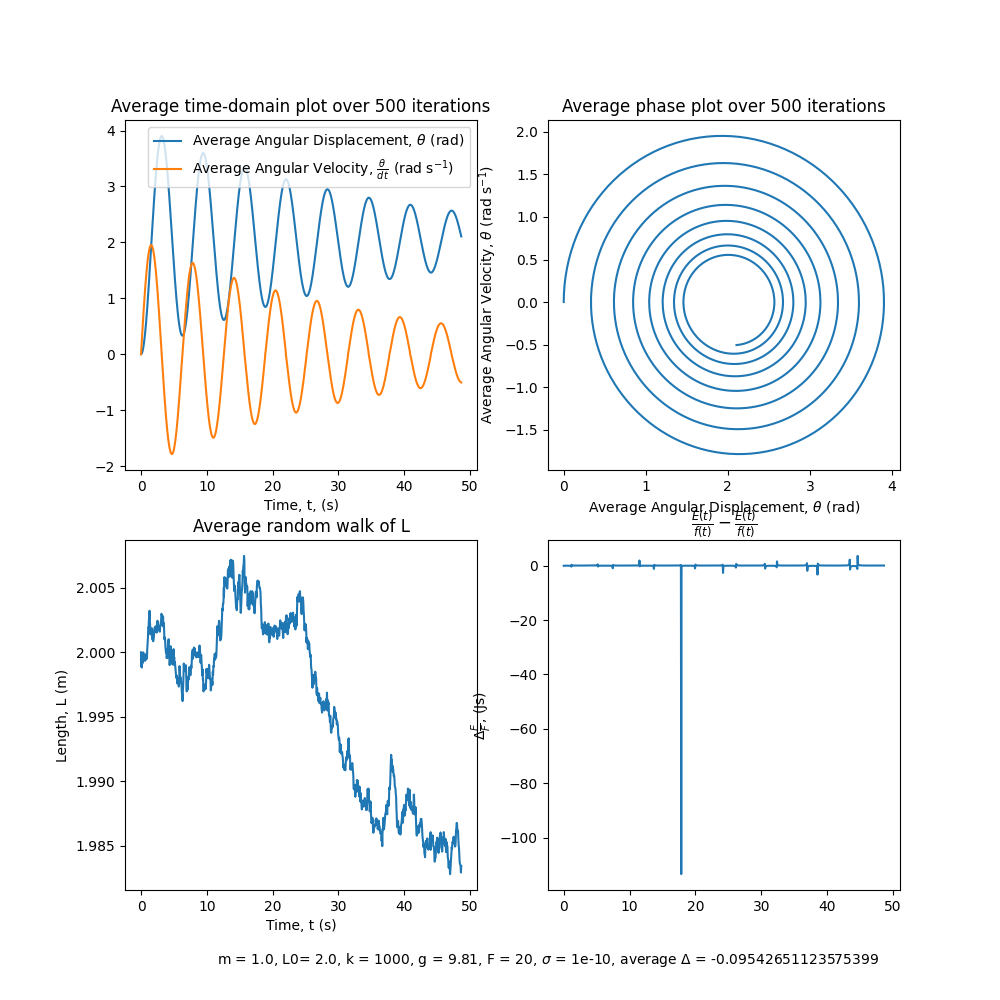
\includegraphics[width = \columnwidth]{Projects/ForcedSimplePendulum/Plots/m = 1.0, L0= 2.0, k = 1000, g = 9.81, F = 20, sigma = 1e-10, run number 4.png}
    \caption{Fifth Iteration.}
    \label{fig:enter-label}
\end{figure}

\begin{figure}
    \centering
    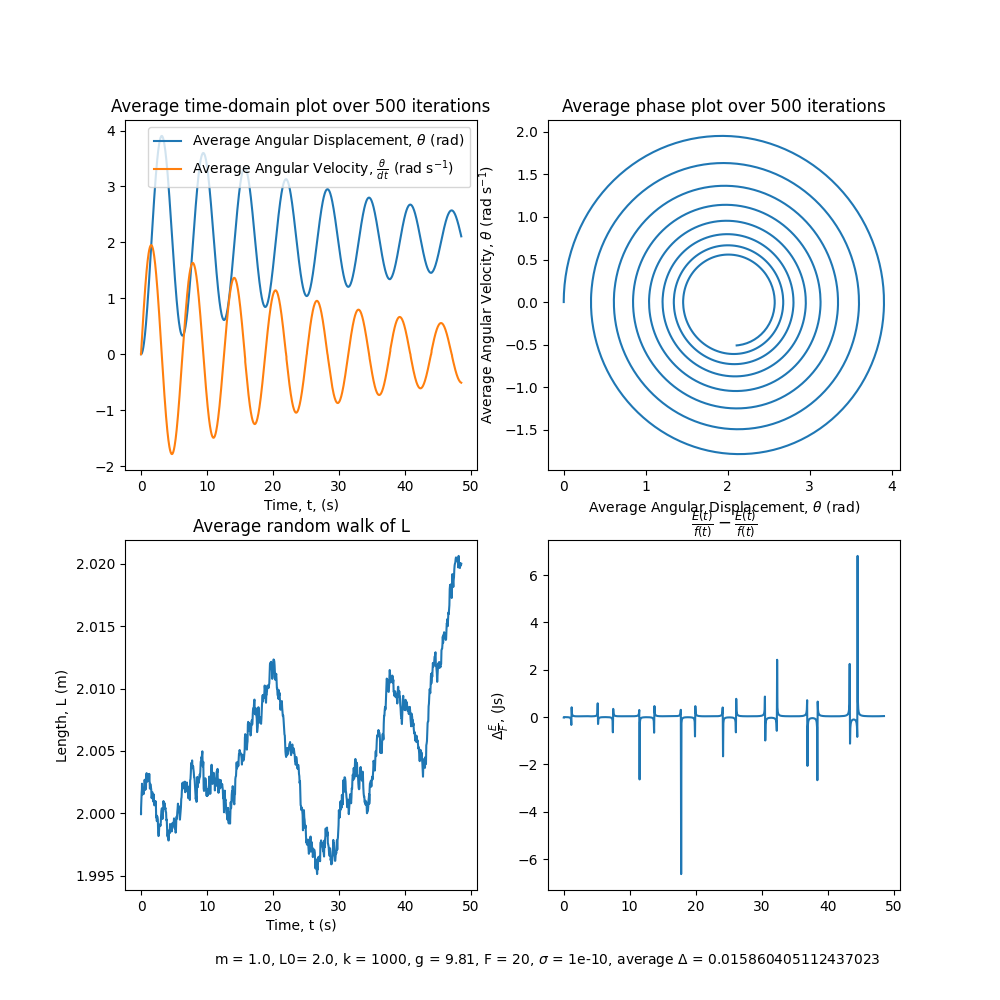
\includegraphics[width = \columnwidth]{Projects/ForcedSimplePendulum/Plots/m = 1.0, L0= 2.0, k = 1000, g = 9.81, F = 20, sigma = 1e-10, run number 5.png}
    \caption{Sixth Iteration.}
    \label{fig:enter-label}
\end{figure}

\begin{figure}
    \centering
    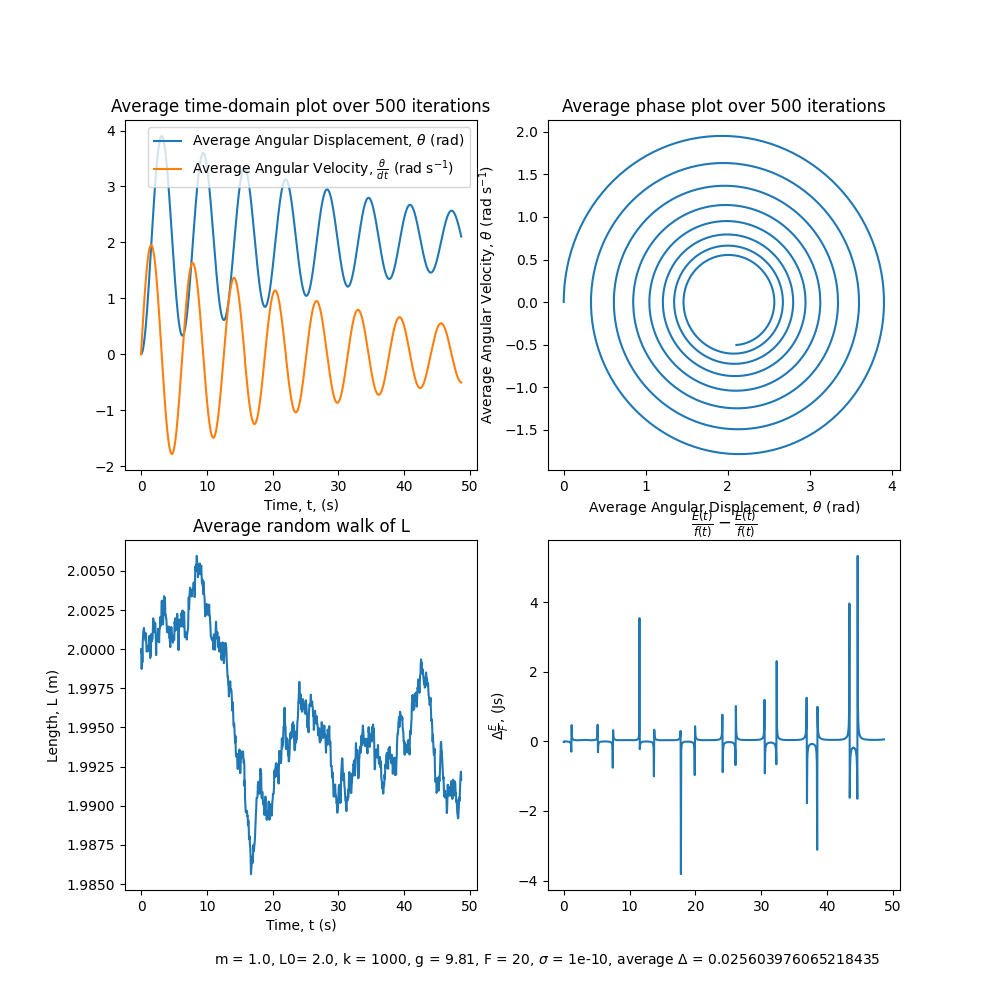
\includegraphics[width = \columnwidth]{Projects/ForcedSimplePendulum/Plots/m = 1.0, L0= 2.0, k = 1000, g = 9.81, F = 20, sigma = 1e-10, run number 6.png}
    \caption{Seventh Iteration.}
    \label{fig:enter-label}
\end{figure}

\begin{figure}
    \centering
    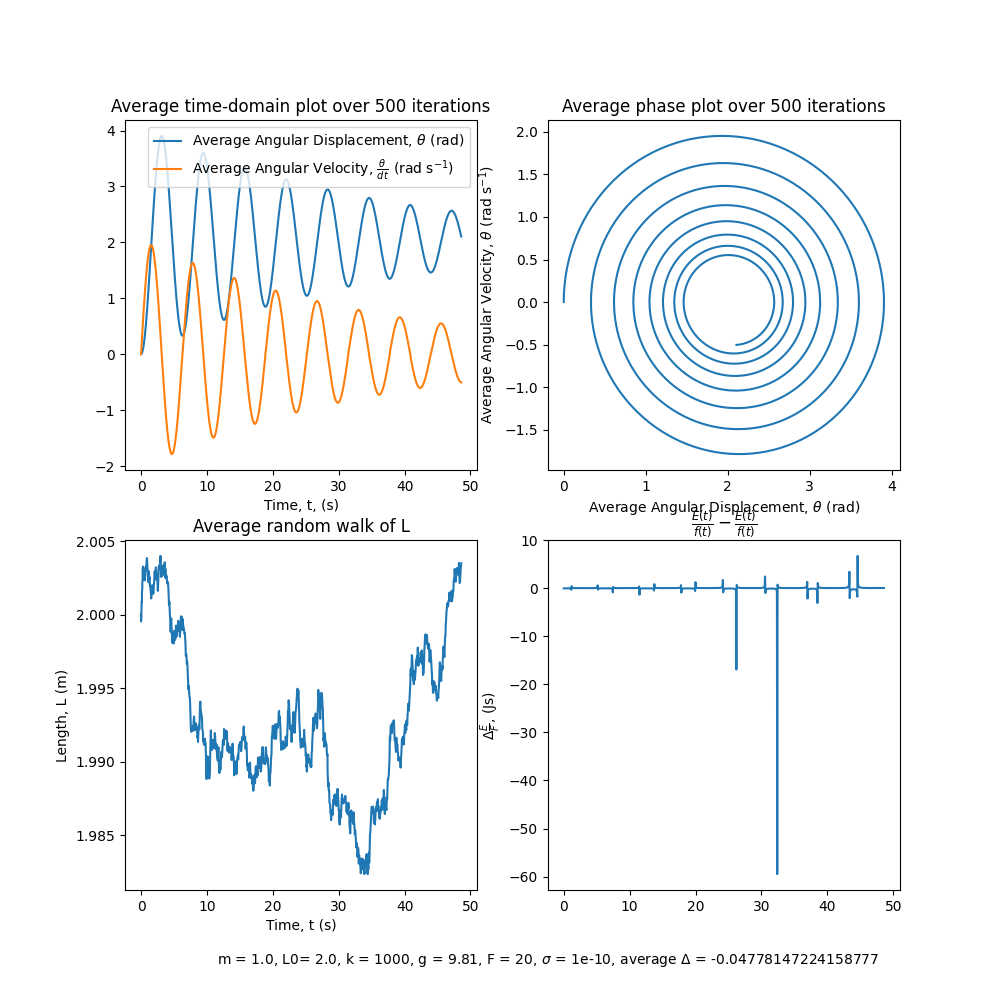
\includegraphics[width = \columnwidth]{Projects/ForcedSimplePendulum/Plots/m = 1.0, L0= 2.0, k = 1000, g = 9.81, F = 20, sigma = 1e-10, run number 7.png}
    \caption{Eighth Iteration.}
    \label{fig:enter-label}
\end{figure}

\begin{figure}
    \centering
    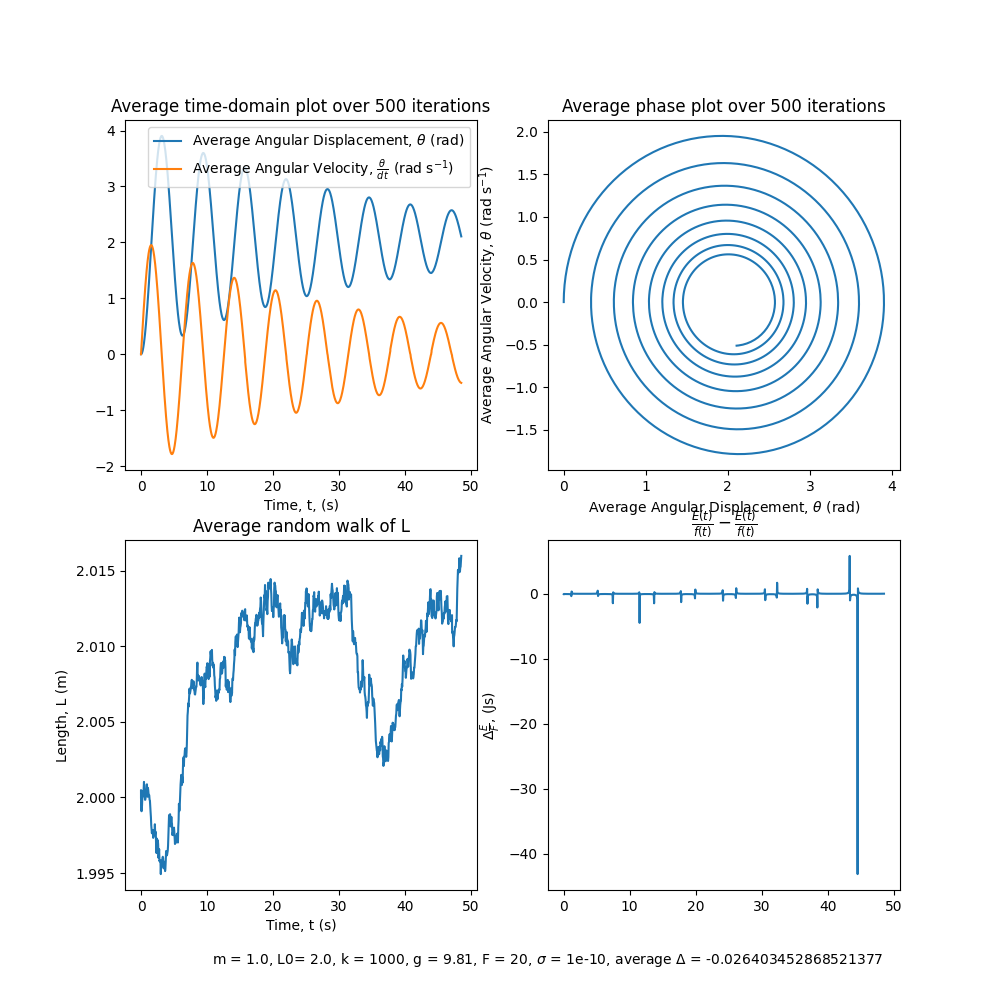
\includegraphics[width = \columnwidth]{Projects/ForcedSimplePendulum/Plots/m = 1.0, L0= 2.0, k = 1000, g = 9.81, F = 20, sigma = 1e-10, run number 8.png}
    \caption{Ninth Iteration.}
    \label{fig:enter-label}
\end{figure}

\begin{figure}
    \centering
    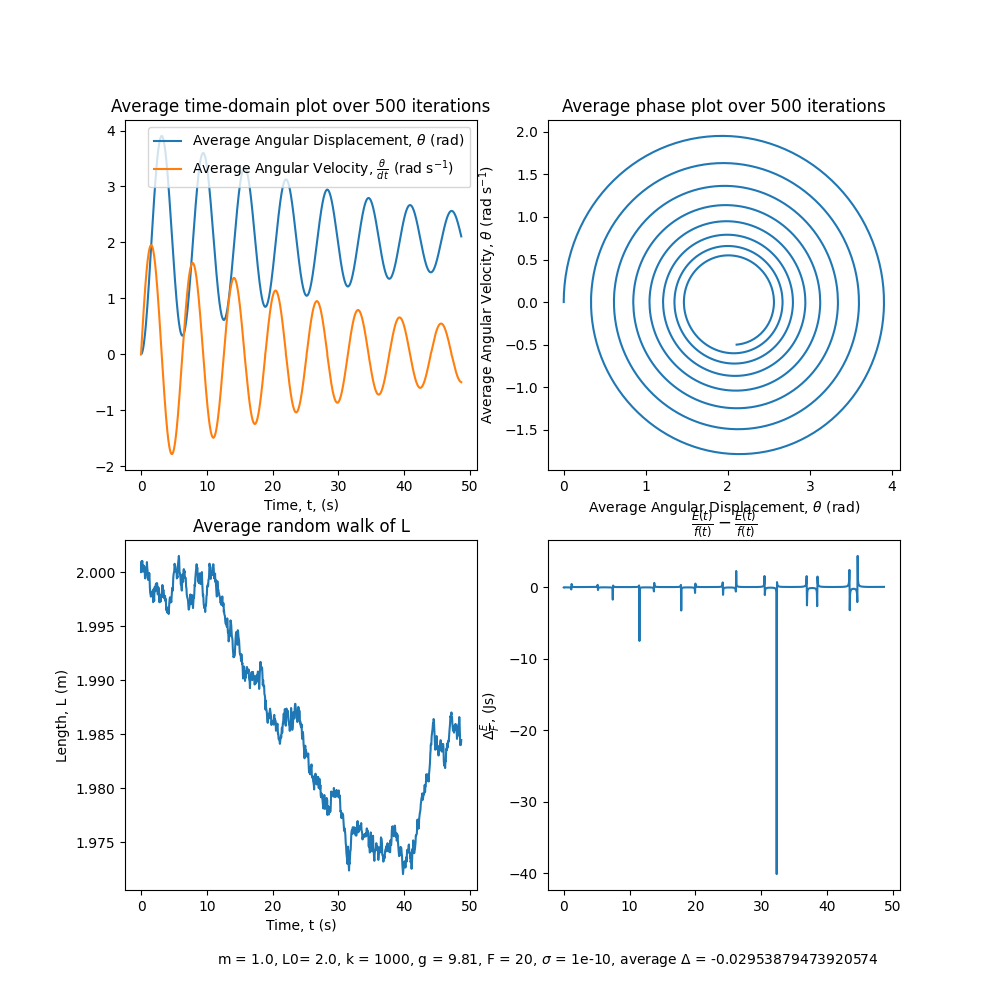
\includegraphics[width = \columnwidth]{Projects/ForcedSimplePendulum/Plots/m = 1.0, L0= 2.0, k = 1000, g = 9.81, F = 20, sigma = 1e-10, run number 9.png}
    \caption{Tenth Iteration.}
    \label{fig:enter-label}
\end{figure}



\section{Analysis}{\label{analysis}}
\subsection{$F \sim{mg}$}{\label{analysisFmg}}
The expected result was that there would be a breakdown in simple harmonic motion as the value of k was decreased. This was true in my case because the pendulum started as a simple harmonic oscillator (Fig. \ref{k 50 to 10} and \ref{Phase plot of k 50 to 10}) but ended up doing complete oscillations (Fig. \ref{k 1 to 0.1}) as the value of k decreased. The case of $k$ from 5 to 1 (see graph of $k = 2$ in Fig. \ref{k 5 to 1 short}) at first glance seemed like there would be some discovery to be done -- it looked to me that there might be a periodicity in the waveform\footnote{like the cover art of Artic Monkey's album AM}, so I increased the integration time period. However, the reality was that it was just the pendulum building up to reach a constant peak amplitude, as seen in Fig. \ref{k 5 to 1 med} and also Fig \ref{k 5 to 1 long}.\\
\\
Regarding the specific damping constant $k = 0.41$ (Fig. \ref{k = 0.41}), there was a \textbf{full oscillation} happening around $t \sim{30}$. I hypothesised was due to the resonance -- forcing frequency $\approx$ natural frequency, so the pendulum had enough energy to make a full oscillation. However as the value of $k$ decreased, the magnitude of the damping term was not enough to keep the resonance under control.

\subsection{Rayleigh Lorentz Pendulum Random Walk}
The goal was to test if the change of L in the case of a random walk allowed the R-L pendulum to remain adiabatically invariant. The random walk followed a normal distribution with $\sigma = 10^{-20}$ with a mean of 0. The most important graphs were the comparison between the random walk in L and the difference between $\frac{E(t)}{f(t)}$ and $\frac{E(0)}{f(0)}$. If said differences were so small to the point that it is negligible, it could be hypothesised that the random walk (following a normal distribution) for the Rayleigh-Lorentz pendulum is adiabatically invariant (because adiabatic invariance requires time in between 2 endpoints to be almost infinite). From the results shown in Section \ref{rlresults}, the average $|Delta\frac{E}{f}$ ranged from $10^{}$ to $10^{}$. Due to the large range of values, I cannot conclude that the change of L in the case of a random walk allows the system to remain adiabatically invariant.

\section{Conclusion}
This project focused on the forced simple pendulum, where the 2nd-order differential equation was solved numerically using the Runge-Kutta 4(5) (RK4(5)) method.

First, in the forced simple pendulum, the pendulum was affected by an external force that was almost equal to its mass. At large values of the damping coefficient, $k$, the system exhibited the behaviour of a simple harmonic oscillator. As the value of $k$ decreased, up to $k\approx 0.41$, the pendulum started doing full rotations due to the resonance of the forcing frequency and the natural frequency of the pendulum.

Next, the forcing frequency was changed out for the change in the length of the pendulum -- akin to the Rayleigh-Lorentz pendulum, which is a form of a forced simple pendulum. The change in length was determined by a random walk that followed a normal distribution. For each step of numerical integration done in the RK4(5) method, the length was changed dynamically with each step. The next value of L was determined by the last value + a random value from the distribution. After many iterations, it was concluded that the difference between the ratio of energy to frequency at t = 0 was not always equal to the ratio of energy to frequency at other, and the average difference ranged from , which showed that this case of the pendulum was not adiabatically invariant. Future work could involve extending the Rayleigh-Lorentz pendulum to the case of a double pendulum and also rather than relying on a random walk to determine the pendulum's length variations, employing a non-linear function could offer a more structured approach. 
\newpage
\section{Addendum} %complete
This section outlines 3 concepts studied in PHYS6017, namely random walks, Monte Carlo simulations, and random walks. A brief description of each concept is stated before some examples in and out of academia are given.
%stuff here
%Show you understand the basics of the technique
% Give 6 examples (including proper references), where the technique has been used in:
% 3 in Academia…
% 3 Outside academia (industry, medicine, finance, etc)
\subsection{Random Walks} %complete
Random walks are a way to generate data. A simple example would be the case of a particle on a 2-D plane, where the particle is allowed to move in one of the four directions possible, and the choice of direction is random, usually according to some probability distribution.

\subsubsection{In Academia} %complete
In \cite{Kruzins1982}, by knowing the sound intensity at a few detection points, sound fields (more specifically, the steady state high-frequency SPL) in non-diffuse spaces can be predicted via random walks, built upon \cite{Gerlach1975}. Random walks have been used in biophysics for an algorithm reconstructing supercoiled DNA \cite{Baba2020} (supercoiled meaning the amount of "twist" in a DNA strand, thereby giving the magnitude of strain on it) \cite{Bauer1980}. The DNA is found to take a random walk, which can be tied to the travelling salesman problem. Furthermore, mapping random walks onto complex network structures (where the moving probability is taken as information flow), and \cite{Noh2004} discovered that information had a directional flow (when random walks were mapped), as opposed to a bidirectional flow (along the backbone of a network). 

\subsubsection{Outside of Academia} %complete
Random walks were used in cybersecurity, where cyber threats were detected via a "self-avoiding" (random) walk \cite{Nia2016}. The patterns were extracted and compared to a threat database. Random walks were also used to predict pedestrian and vehicular movement in London \cite{Hanna2021}, and proved to be very effective, compared to segment-based centrality measures \cite{Jayasinghe2015}. A random walk was also used in a simple risk business \cite{Seal1966}, seeing the probability of ruin as the number of contracts go up.

\subsection{Monte Carlo Simulations} %complete
Prevalent in the world of finance, physics, engineering, statistics and many more, the famous casino in Monte Carlo was an inspiration to the Monte Carlo simulation. It is a way to solve complex problems typically involving many variables, which may be challenging to solve analytically. They rely on randomness to generate large numbers of outcomes via simulations, where probabilities or expectation values can be calculated.

\subsubsection{In Academia} %complete
The Monte Carlo (MC) method was used to do a simulation of the Ising model in 2-D \cite{Shekaari2021}\cite{Jindal2007}, a very important model in statistical mechanics. It is also used in robotics, where it is used to improve the localisation of a moving robot in a dynamic environment \cite{Zhao2008} by using a vision-based MC localization. MC method is also used in machine learning for gradient estimation - the pathwise, score function and measure-valued gradient estimators were used \cite{Mohamed2020}.

\subsubsection{Outside of Academia} %complete
Many applications were developed for proton therapy using the Monte Carlo method, such as VMCpro \cite{FippelSoukup2004} (patient dose calculation), MCNPX \cite{Waters2002}, FLUKA \cite{Ferrari2005} and Geant4 \cite{Geant4} \cite{Geant4_2} (all-particle code that can work with motion and magnetic fields). TOPAS (TOol for PArticle Simulation) \cite{Perl2012}\cite{Faddegon2020} was then developed using the Geant4 toolkit to make it more accessible to medical physicists, radiobiologists and clinicians. Other than proton therapy, the MC method is used in risk analysis of the energy efficiency investments in buildings \cite{Togashi2019}, by calculating the probability distribution of energy reduction. MC method is also used in quality control \cite{Moran2023}. The important characteristics of a product can be identified, allowing the manufacturer to prioritise certain aspects of their product to ensure customer satisfaction.

\subsection{Random Numbers} %complete
Random numbers are numbers generated randomly where the current number generated has no relationship to the previous number generated, and neither will the current number affect the next. They are used extensively in fields such as cryptography and statistics.

\subsubsection{In Academia}
An efficient stock market resembles a random number generator \cite{Doyle2013}. Therefore, random numbers were used to test the Efficient Market Hypothesis (EMH) \cite{Yen2008} by using the Overlapping Serial Test \cite{Good1953}, a form of test for randomness. Randomised numerical linear algebra \cite{Martinsson2020} could be applied to statistics \cite{Gentle2012}. Random numbers have been used in investigating access games by having a random number of players \cite{Tembine2008}.

\subsubsection{Outside of Academia} %complete
True random number generators (TRNG), as outlined in \cite{Sunar2009} are used in cryptography (where the TRNG has to meet certain criteria \cite{Latham2001}). TRNG was also used in audio encryption \cite{Etem2020}. Following the (not so recent) cryptocurrency boom, blockchain-based random number generators \cite{Hsieh2022} are explored and their uses in blockchain games \cite{Du2019}. Random numbers are also used in clinical trials \cite{Beller2002}, which assign participants to either of the available groups (i.e. a placebo and non-placebo group for a vaccine test).

\newpage
\section{Bibliography}
\bibliographystyle{apalike}
\bibliography{references}

\onecolumn
\newpage
\section{Appendix A: Phase Plots (or Phase portrait)} \label{phase plots appendix}
Phase plots (meaning plot of $\frac{d^2\theta}{dt^2}$ against $\frac{d\theta}{dt}$ in this case), are different from the usual time-domain plots ($\theta$ against t). The classic time-domain plot is a good way to visualise the change of the pendulum's position over time. The time-domain plots give the oscillation period (thereby the frequency), and amplitude, and it is easy to see if any damping/external forces have been applied to the system (the pendulum). A phase portrait, on the other hand, gives a visualisation of the system's evolution in phase space. The intersection of trajectories at a point (or the approach of trajectories to a point) can indicate equilibrium points, stability (via attractors or repellers), limit cycles (repeated behaviour) or chaotic behaviour.
\begin{figure}[H]
    \centering
    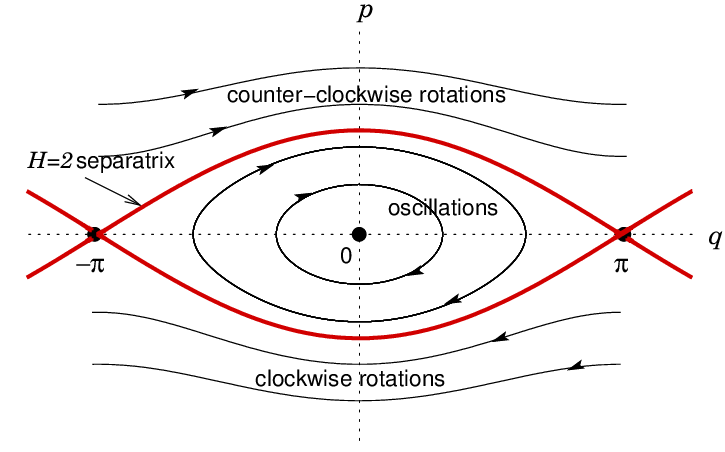
\includegraphics[width = 0.7\columnwidth]{Projects/ForcedSimplePendulum/WrittenReport/figs/The-phase-space-of-the-simple-pendulum.png}
    \caption{Phase plot for a simple pendulum. Taken from \cite{Ball2007}.}
    \label{fig:enter-label}
\end{figure}

\begin{figure}[H]
    \centering  
    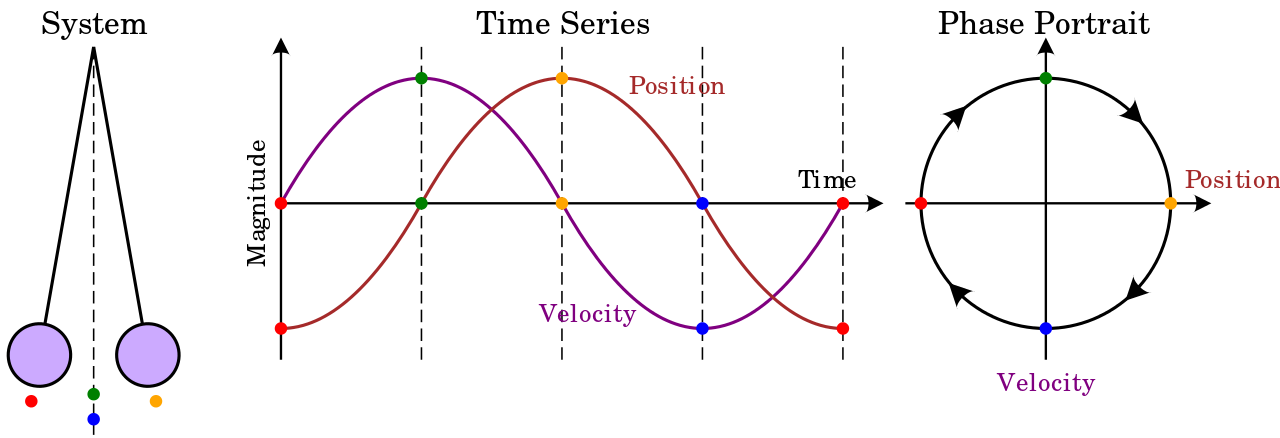
\includegraphics[width = \columnwidth]{Projects/ForcedSimplePendulum/WrittenReport/figs/Pendulum_phase_portrait_illustration.svg.png}
    \caption{How a phase portrait is compared to a time-domain plot for a simple pendulum. The blue dot for the illustration of the system corresponds to the blue dots on the time series graph and the phase portrait (and so do the other coloured dots). Taken from \href{https://commons.wikimedia.org/wiki/File:Pendulum_phase_portrait_illustration.svg}{WikiMedia}.}
    \label{fig:enter-label}
\end{figure}
 It is useful to consider both plots for this project. I will introduce some simple examples of the comparison of time-domain and phase-domain plots.
 \begin{figure}[H]
     \centering
     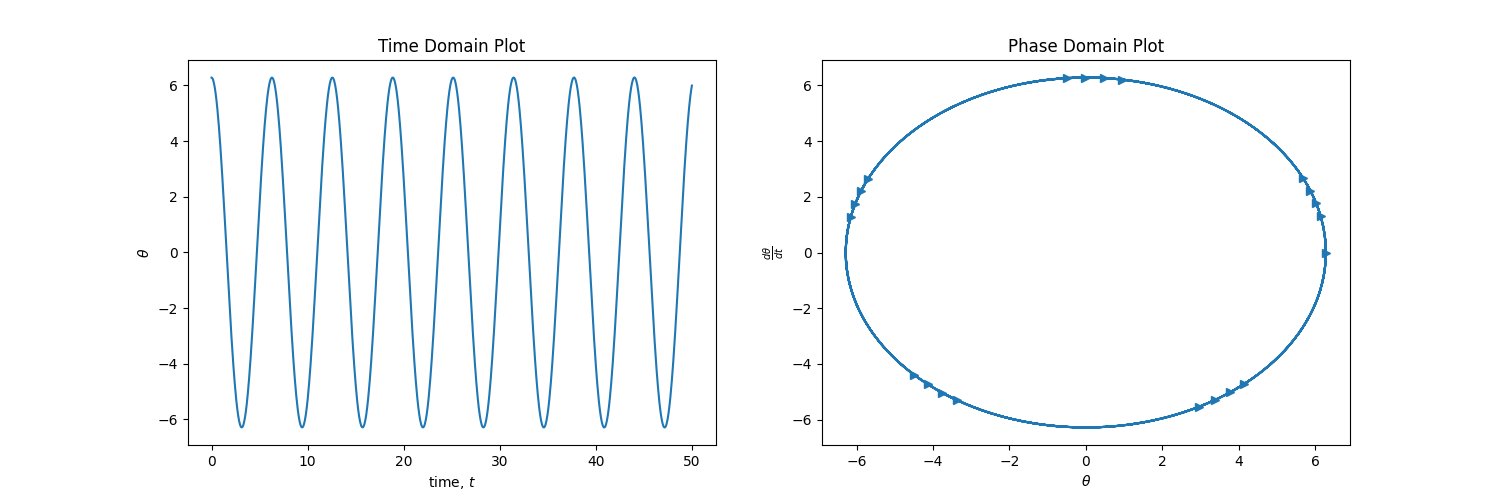
\includegraphics[width = \columnwidth]{Projects/ForcedSimplePendulum/Plots/demo_shm.png}
     \caption{Time and Phase domain plots for simple harmonic motion. \href{https://github.com/linsuong/PHYS-6017-Labs/blob/main/Projects/ForcedSimplePendulum/Plots/demo_shm.gif}{(Animation here)}}
     \label{fig:enter-label}
 \end{figure}

 \begin{figure}[H]
     \centering
     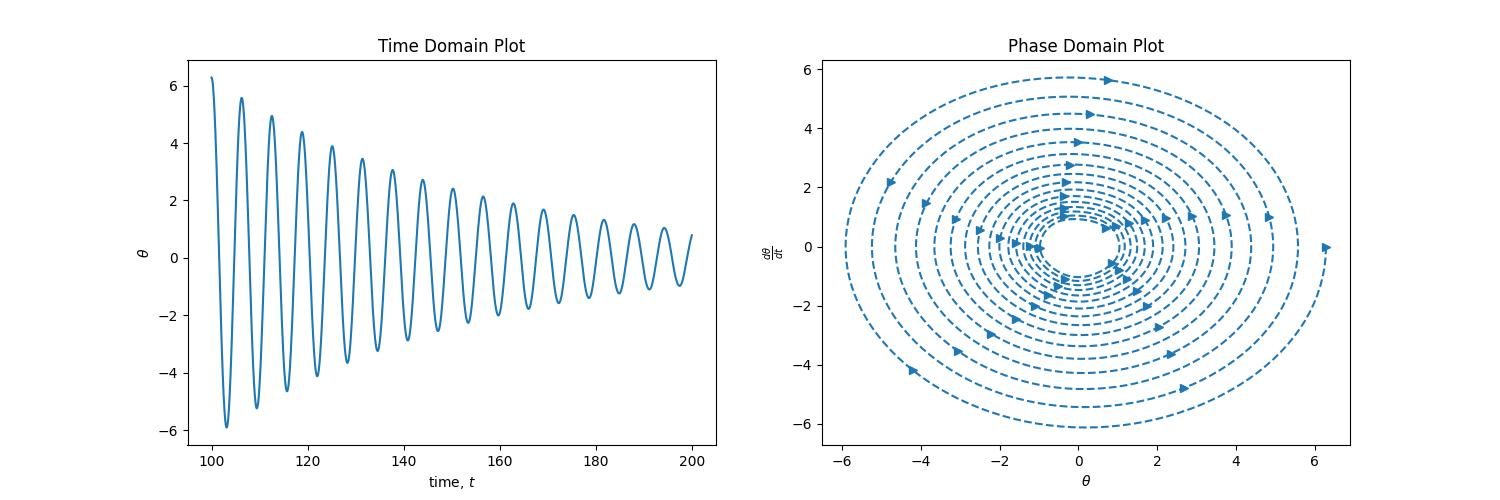
\includegraphics[width = \columnwidth]{Projects/ForcedSimplePendulum/Plots/demo_limit_cycles.jpg}
     \caption{Due to the presence of damping (seen in the time-domain plot), these plots showcase the concept of limit cycles (in the phase-domain plot), where trajectories spiral into each other.}
     \label{fig:enter-label}
 \end{figure}

\begin{figure}[H]
    \centering
    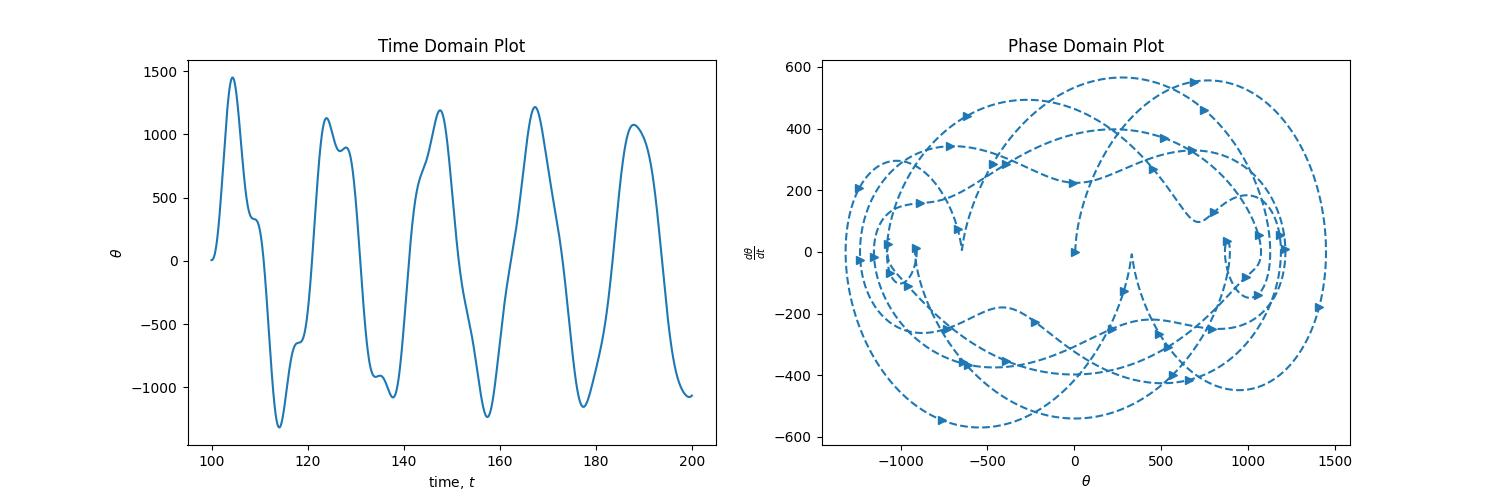
\includegraphics[width = \columnwidth]{Projects/ForcedSimplePendulum/Plots/demo_chaos.jpg}
    \caption{An example of chaotic behaviour. It definitely would not have been obvious just by looking at the time-domain plot alone.\href{https://github.com/linsuong/PHYS-6017-Labs/blob/main/Projects/ForcedSimplePendulum/Plots/demo\%20chaos.gif}{(Animation of a different plot here, but still chaotic)}}
    \label{fig:enter-label}
\end{figure}

\section{Appendix B: Plots for the case of $F \sim{mg}$}{\label{plotsFmg}}
This section contains graphs that have not been used in the main body of the text or are not necessary to show, but showcase the iterative process where I select values of parameters used. Initially, I tested for values of k of a large magnitude:
\begin{figure}
    \centering
    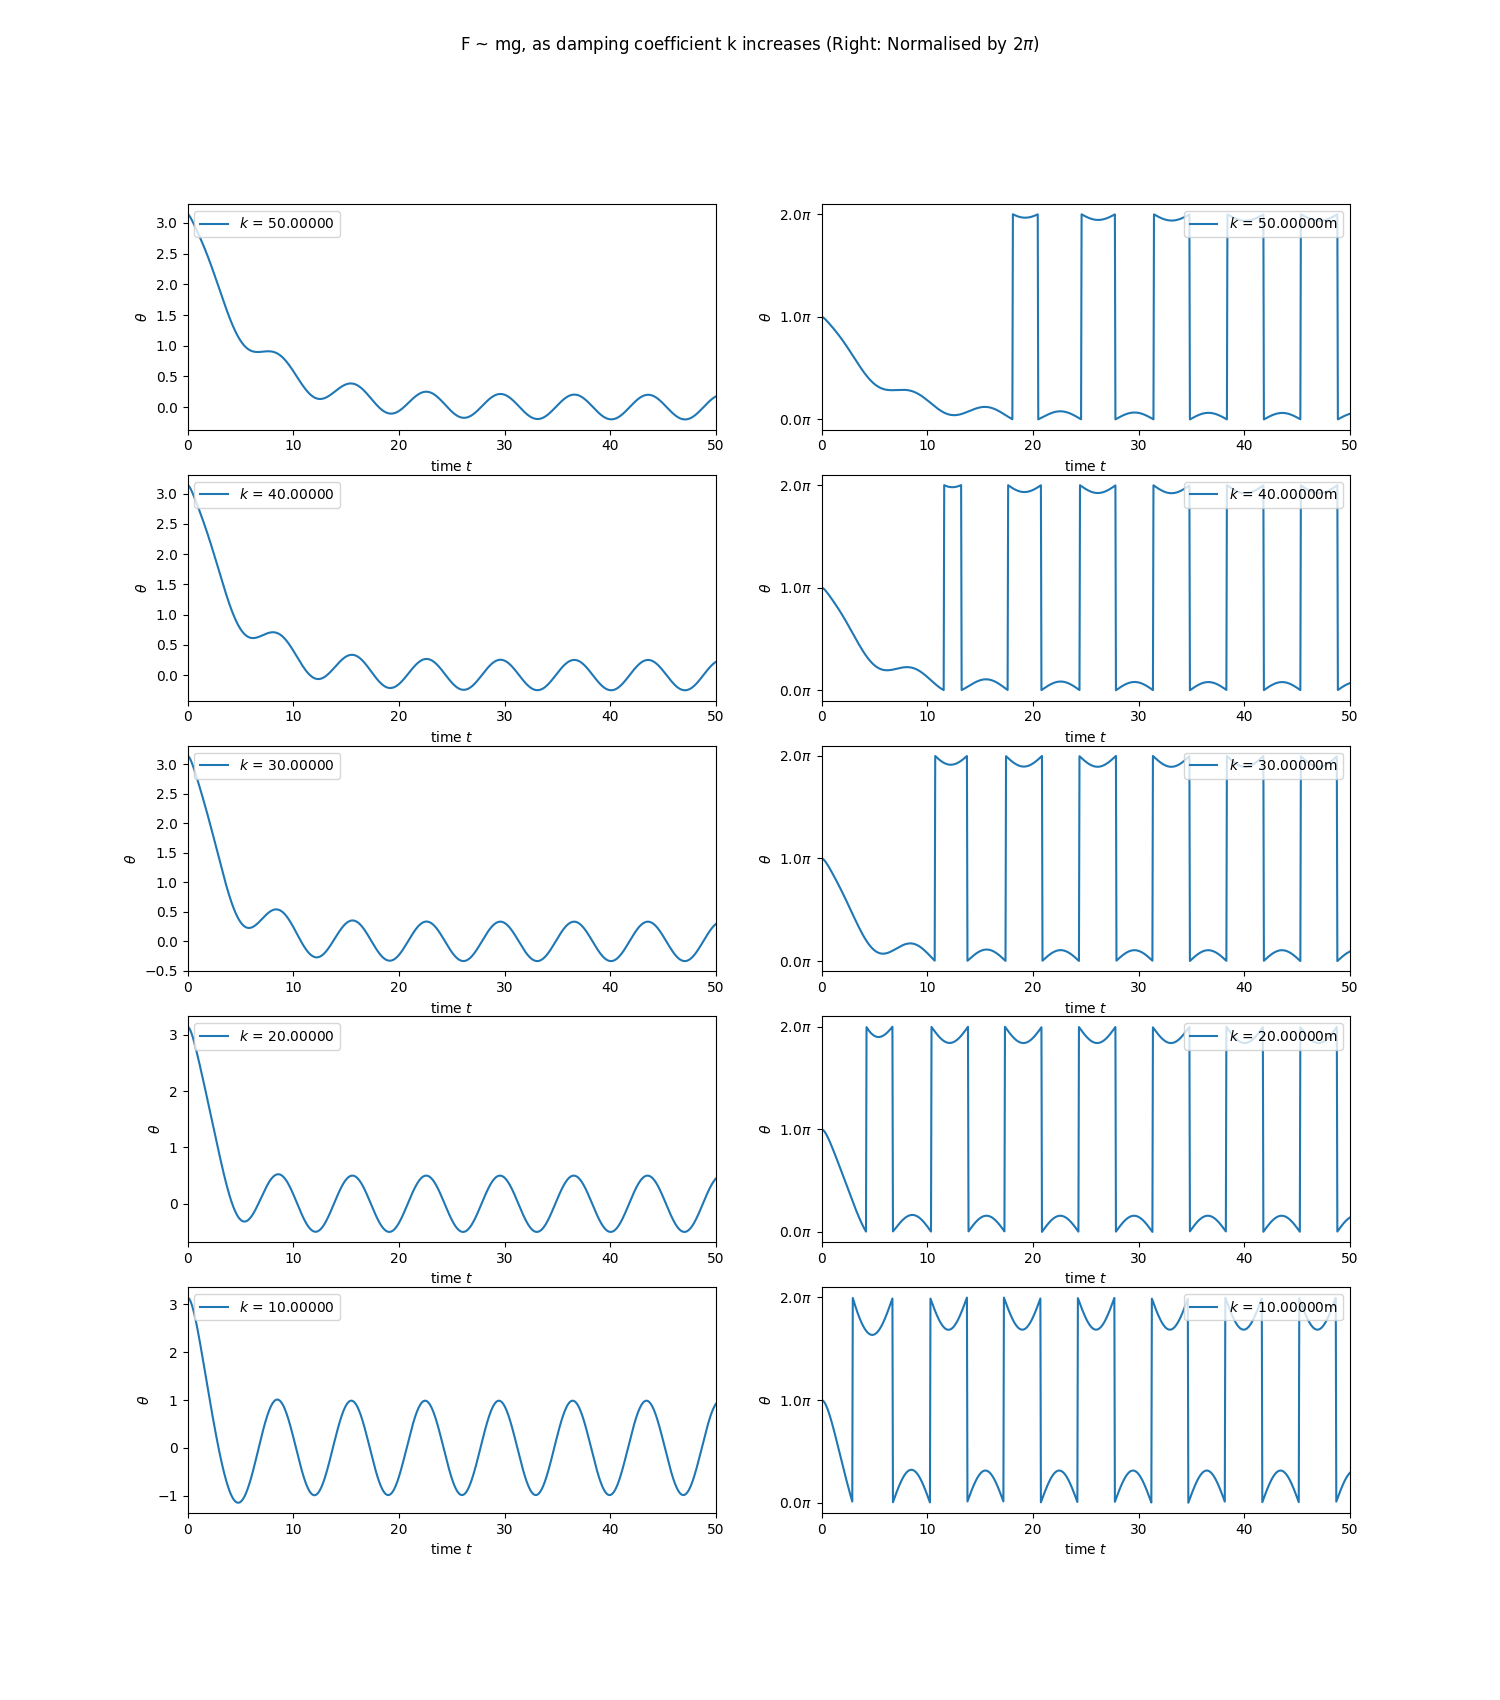
\includegraphics[width = \columnwidth]{Projects/ForcedSimplePendulum/Plots/F~mg as damping coefficient k increases from 50 to 10.png}
    \caption{$F \sim{mg}$ for $k = 50$ to $k = 10$.}
    \label{k 50 to 10}
\end{figure}

\begin{figure}
    \centering
    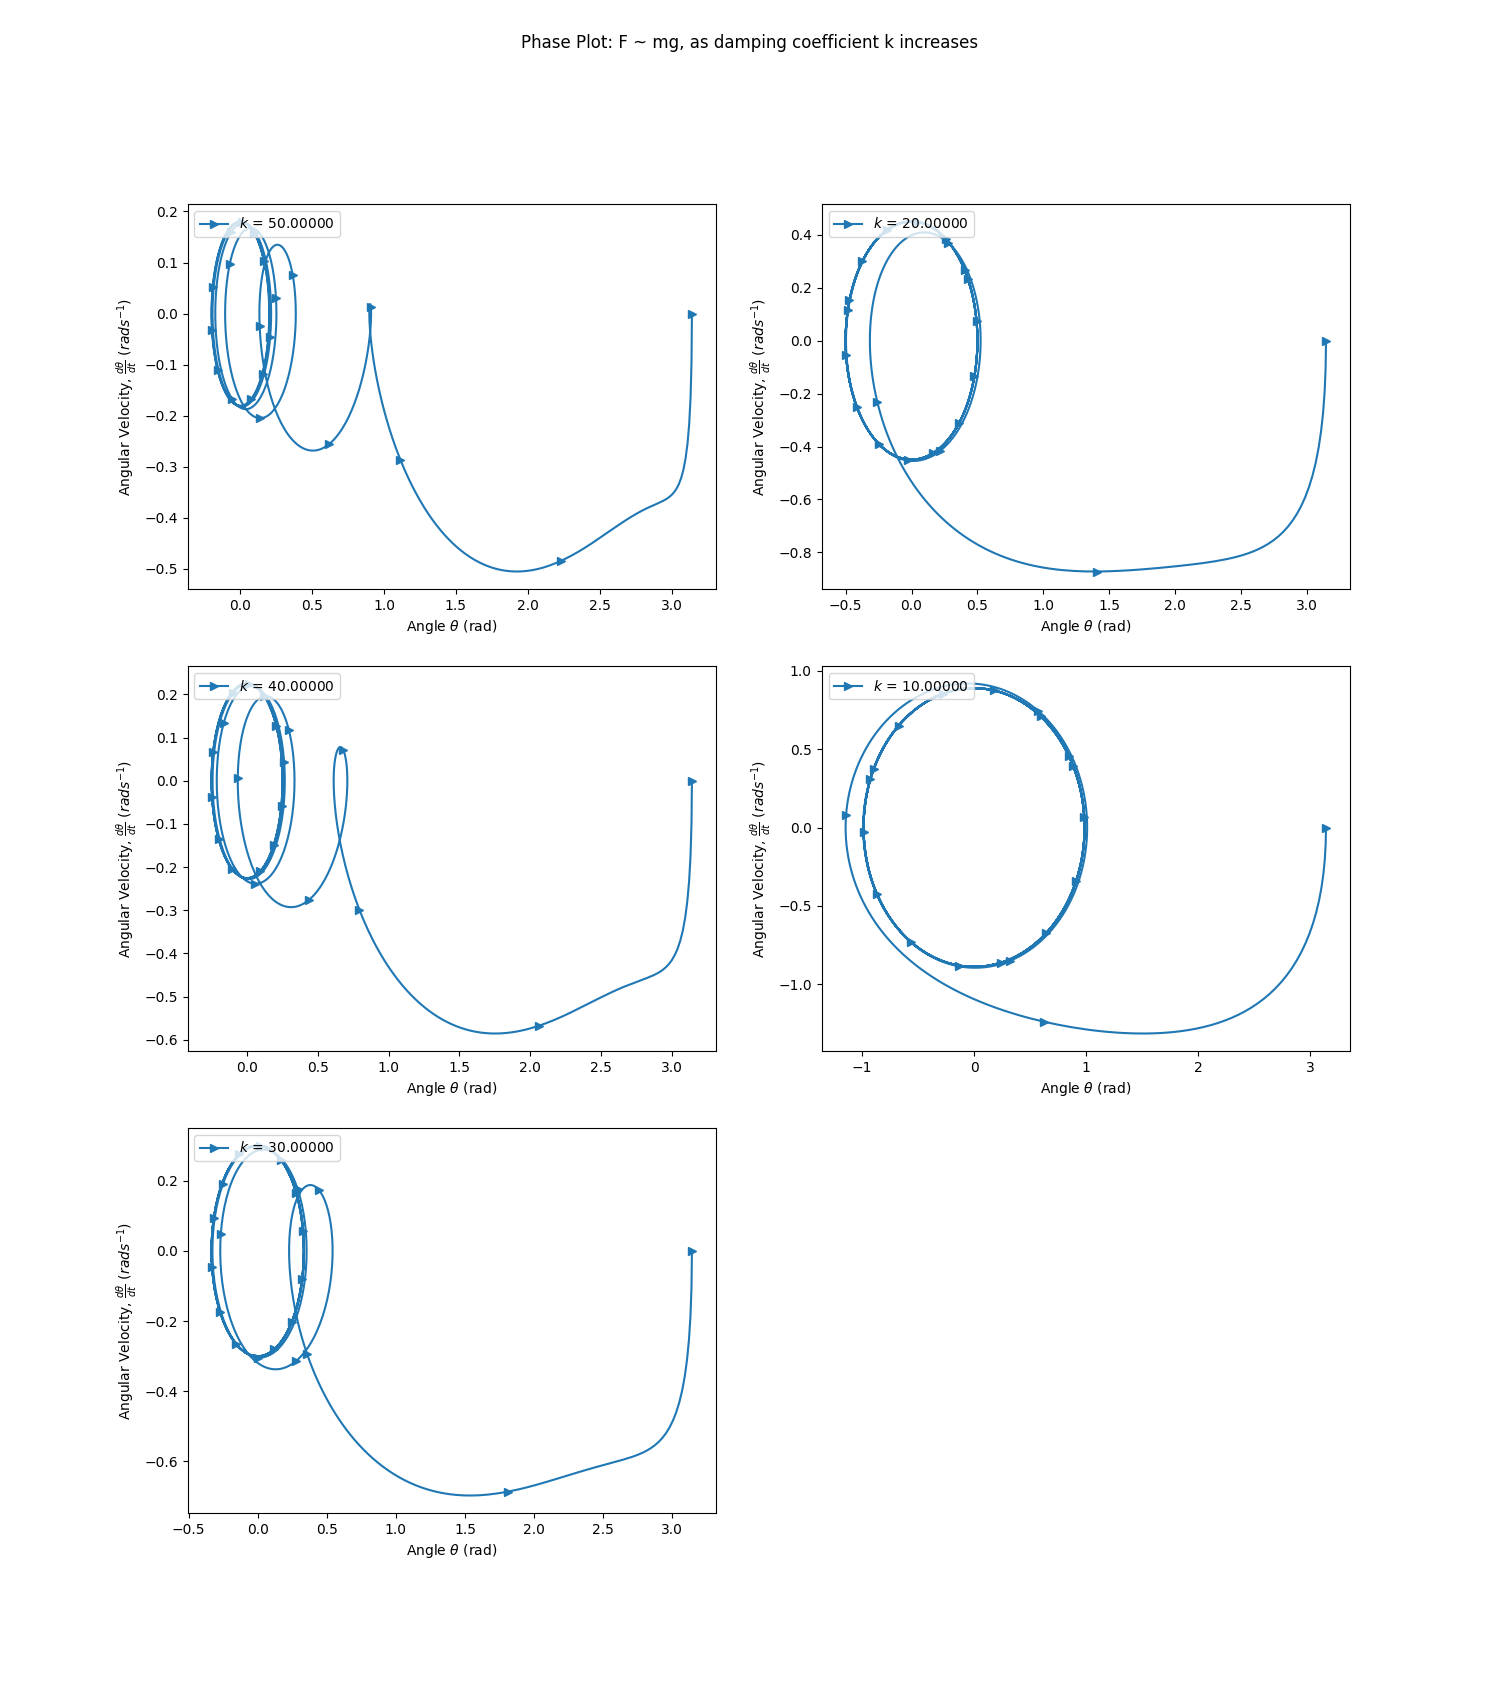
\includegraphics[width = \columnwidth]{Projects/ForcedSimplePendulum/Plots/Phase plot of F~mg as damping coefficient k increases from 50 to 10.png}
    \caption{Phase plot of $F \sim{mg}$ for $k = 5$ to $k = 1$.}
    \label{Phase plot of k 50 to 10}
\end{figure}
From the plots, it just looked to me as if the pendulum was not doing a whole lot - oscillating around the $0/2\pi$ mark, which is the lowest point of the pendulum's motion. I then reduced $k$ from 5 to 1.
\begin{figure}
    \centering
    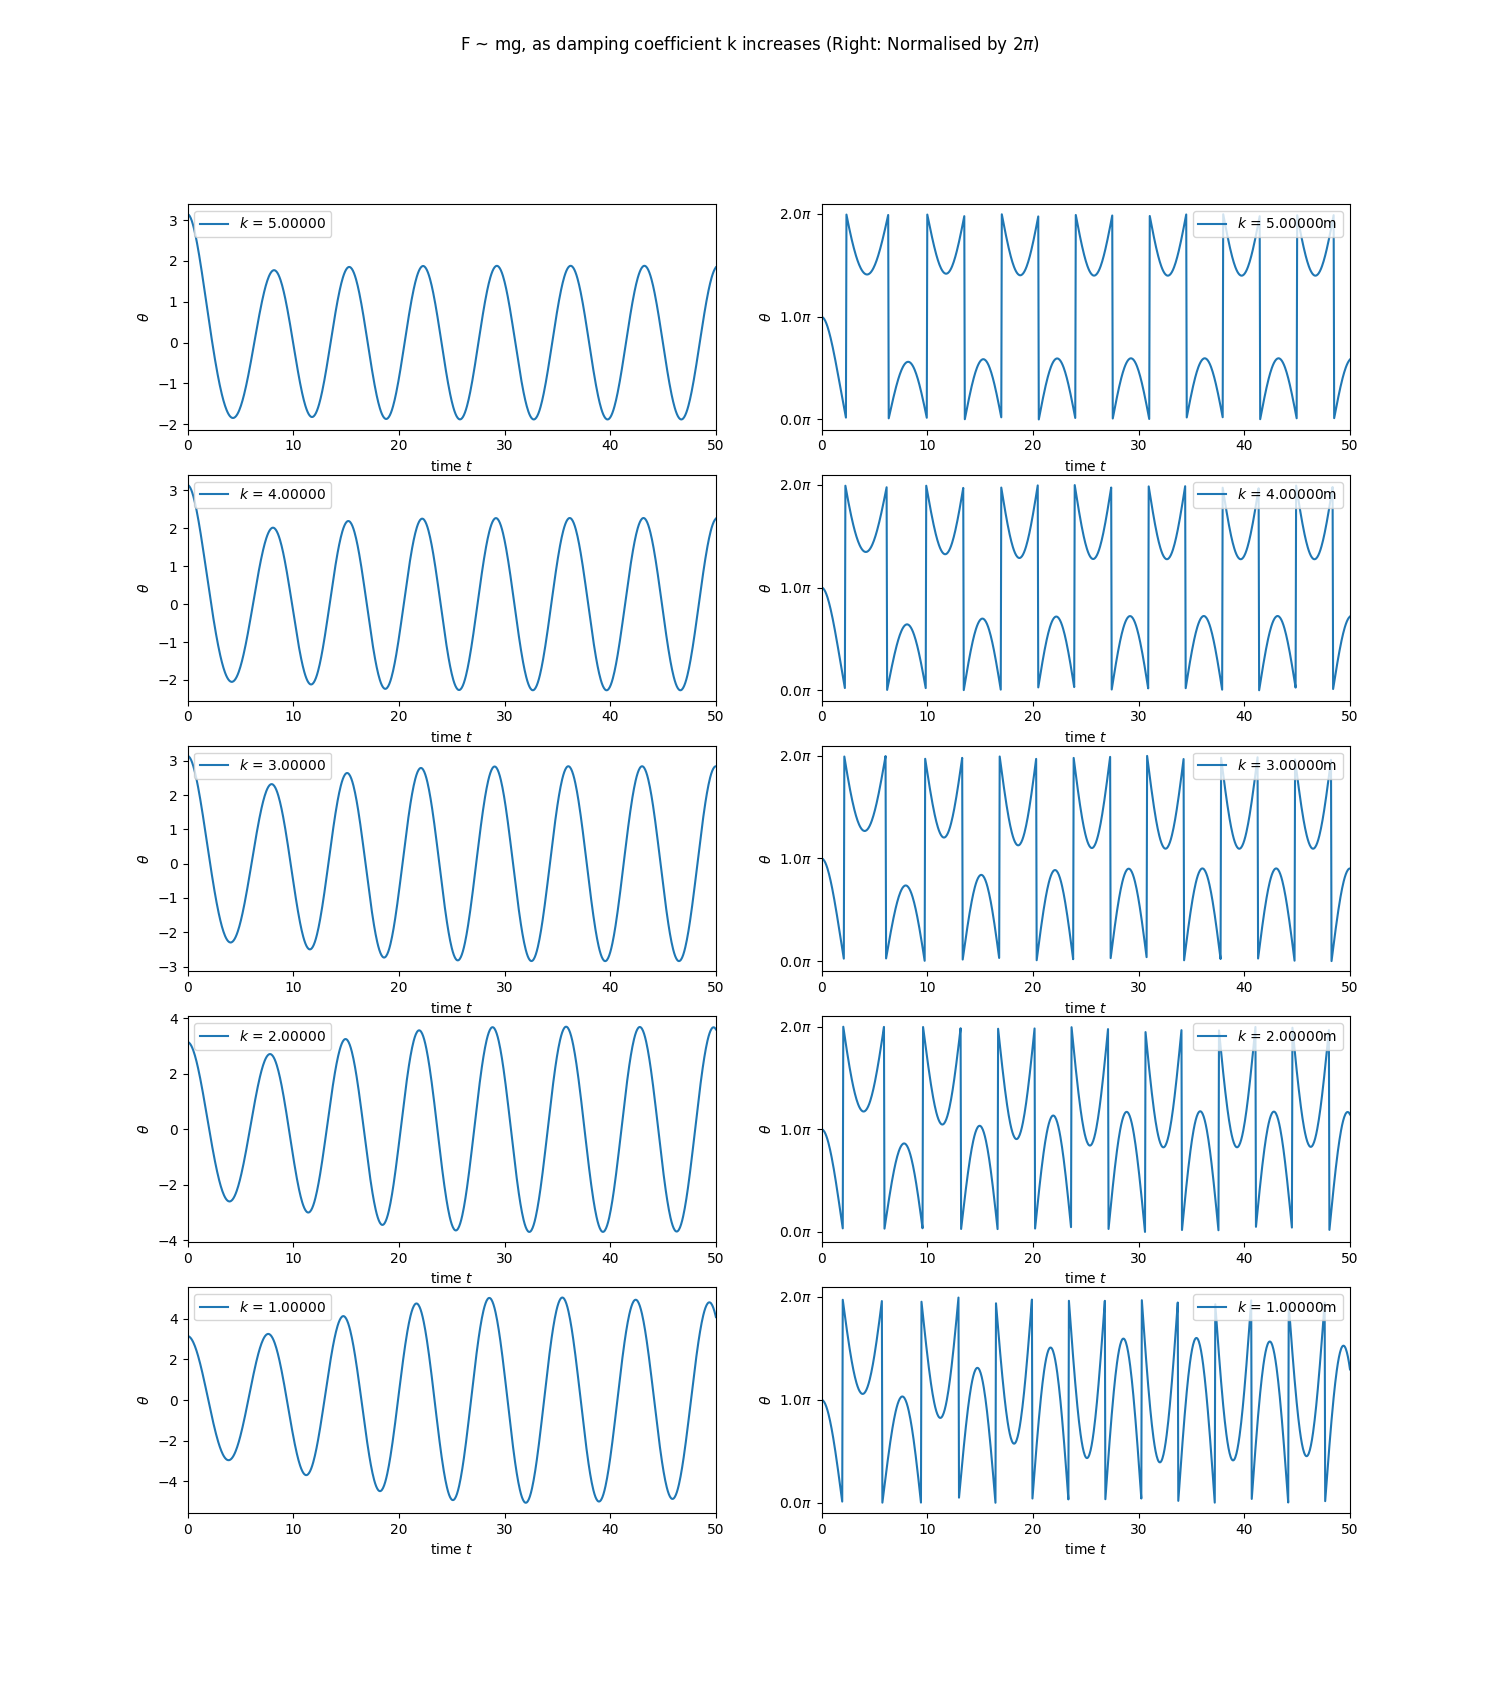
\includegraphics[width = \columnwidth]{Projects/ForcedSimplePendulum/Plots/F~mg as damping coefficient k increases from 5 to 1.png}
    \caption{$F \sim{mg}$ for $k = 5$ to $k = 1$.}
    \label{k 5 to 1}
\end{figure}

\begin{figure}
    \centering
    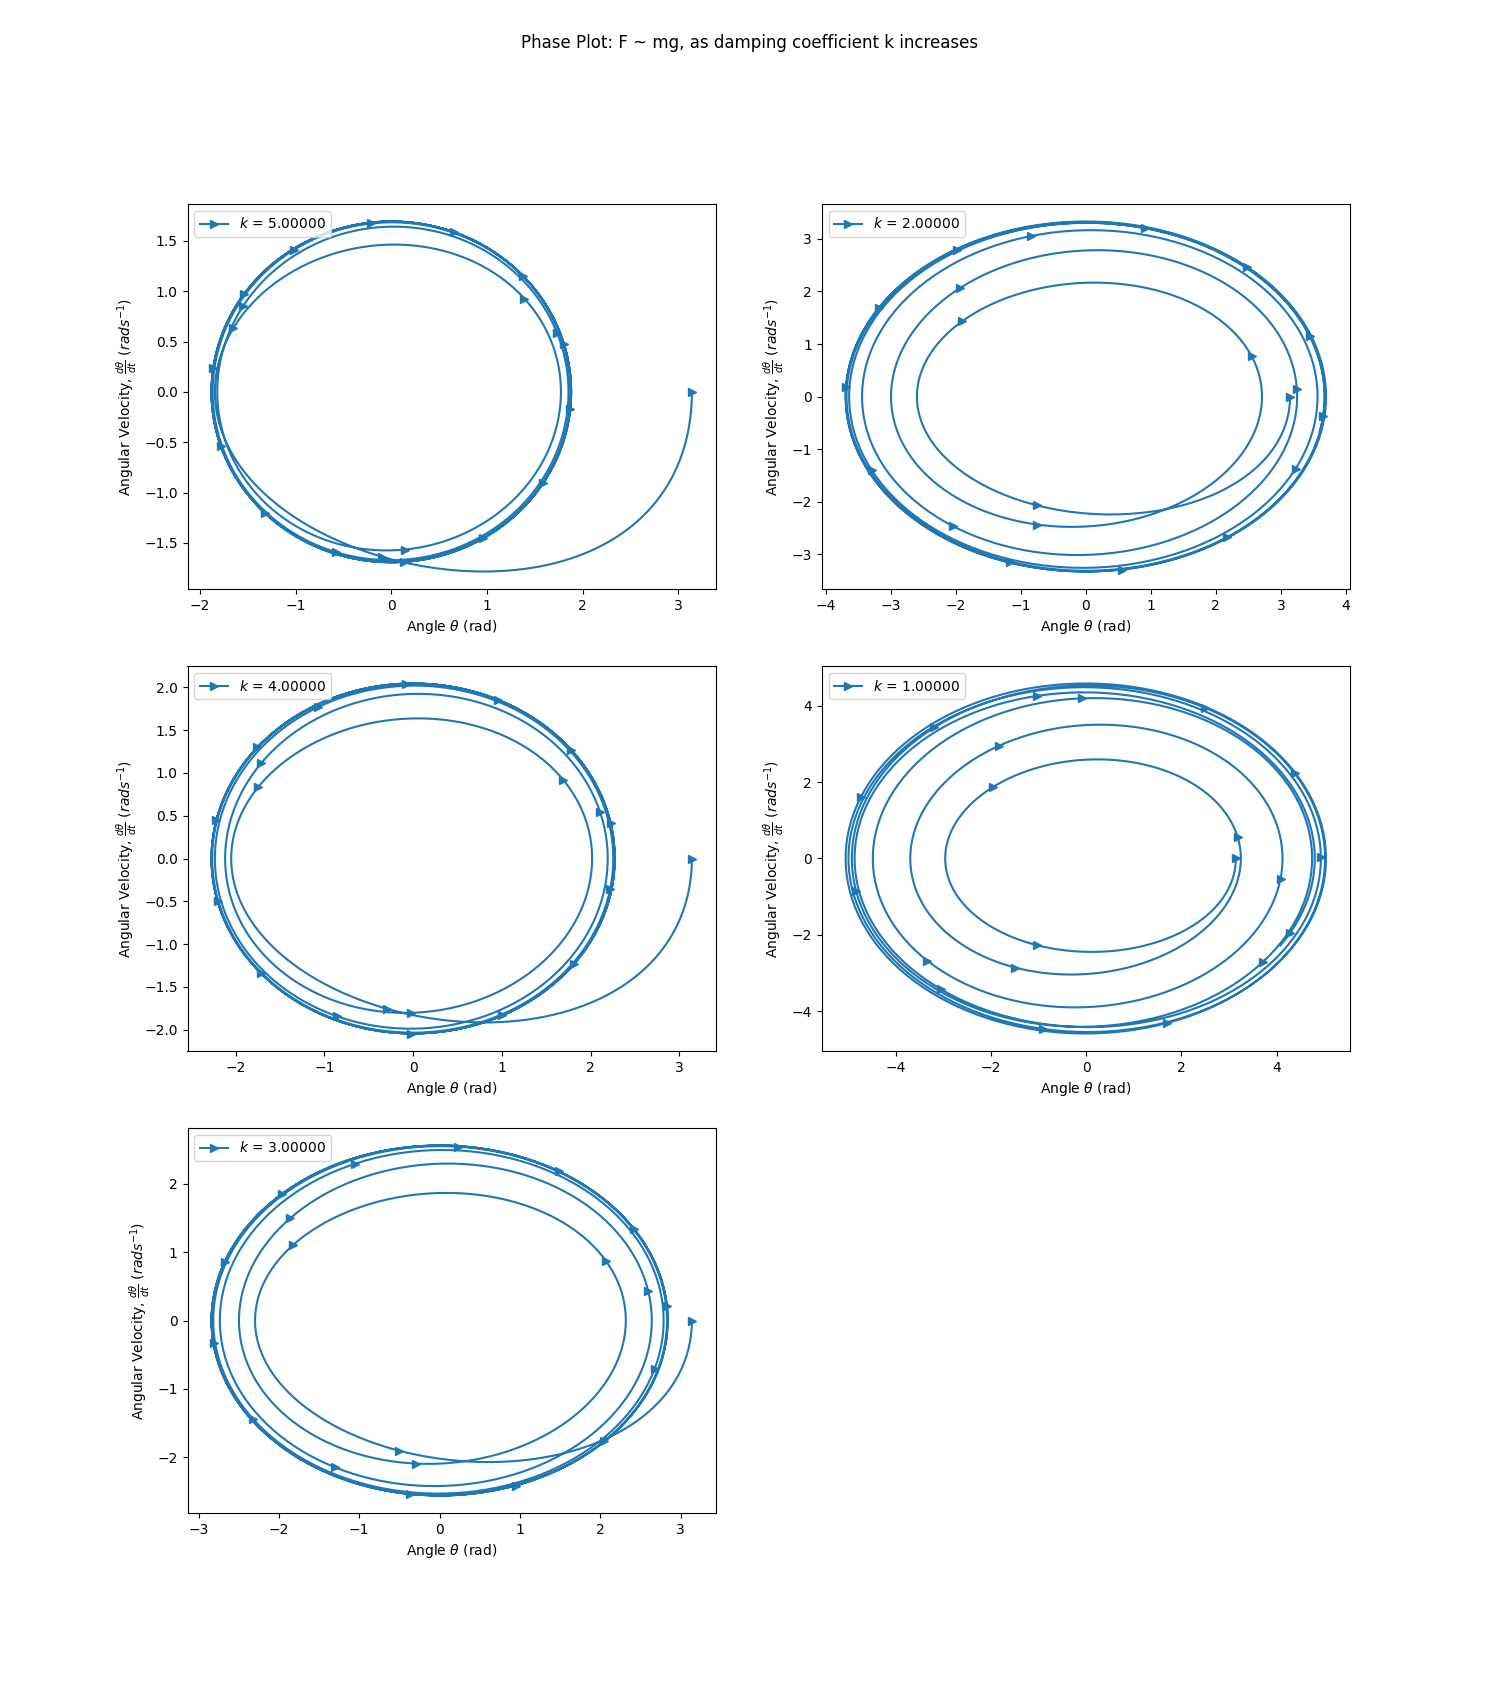
\includegraphics[width = \columnwidth]{Projects/ForcedSimplePendulum/Plots/Phase plot of F~mg as damping coefficient k increases from 5 to 1.png}
    \caption{Phase plot of $F \sim{mg}$ for $k = 5$ to $k = 1$.}
    \label{fig:enter-label}
\end{figure}

\begin{figure}
    \centering
    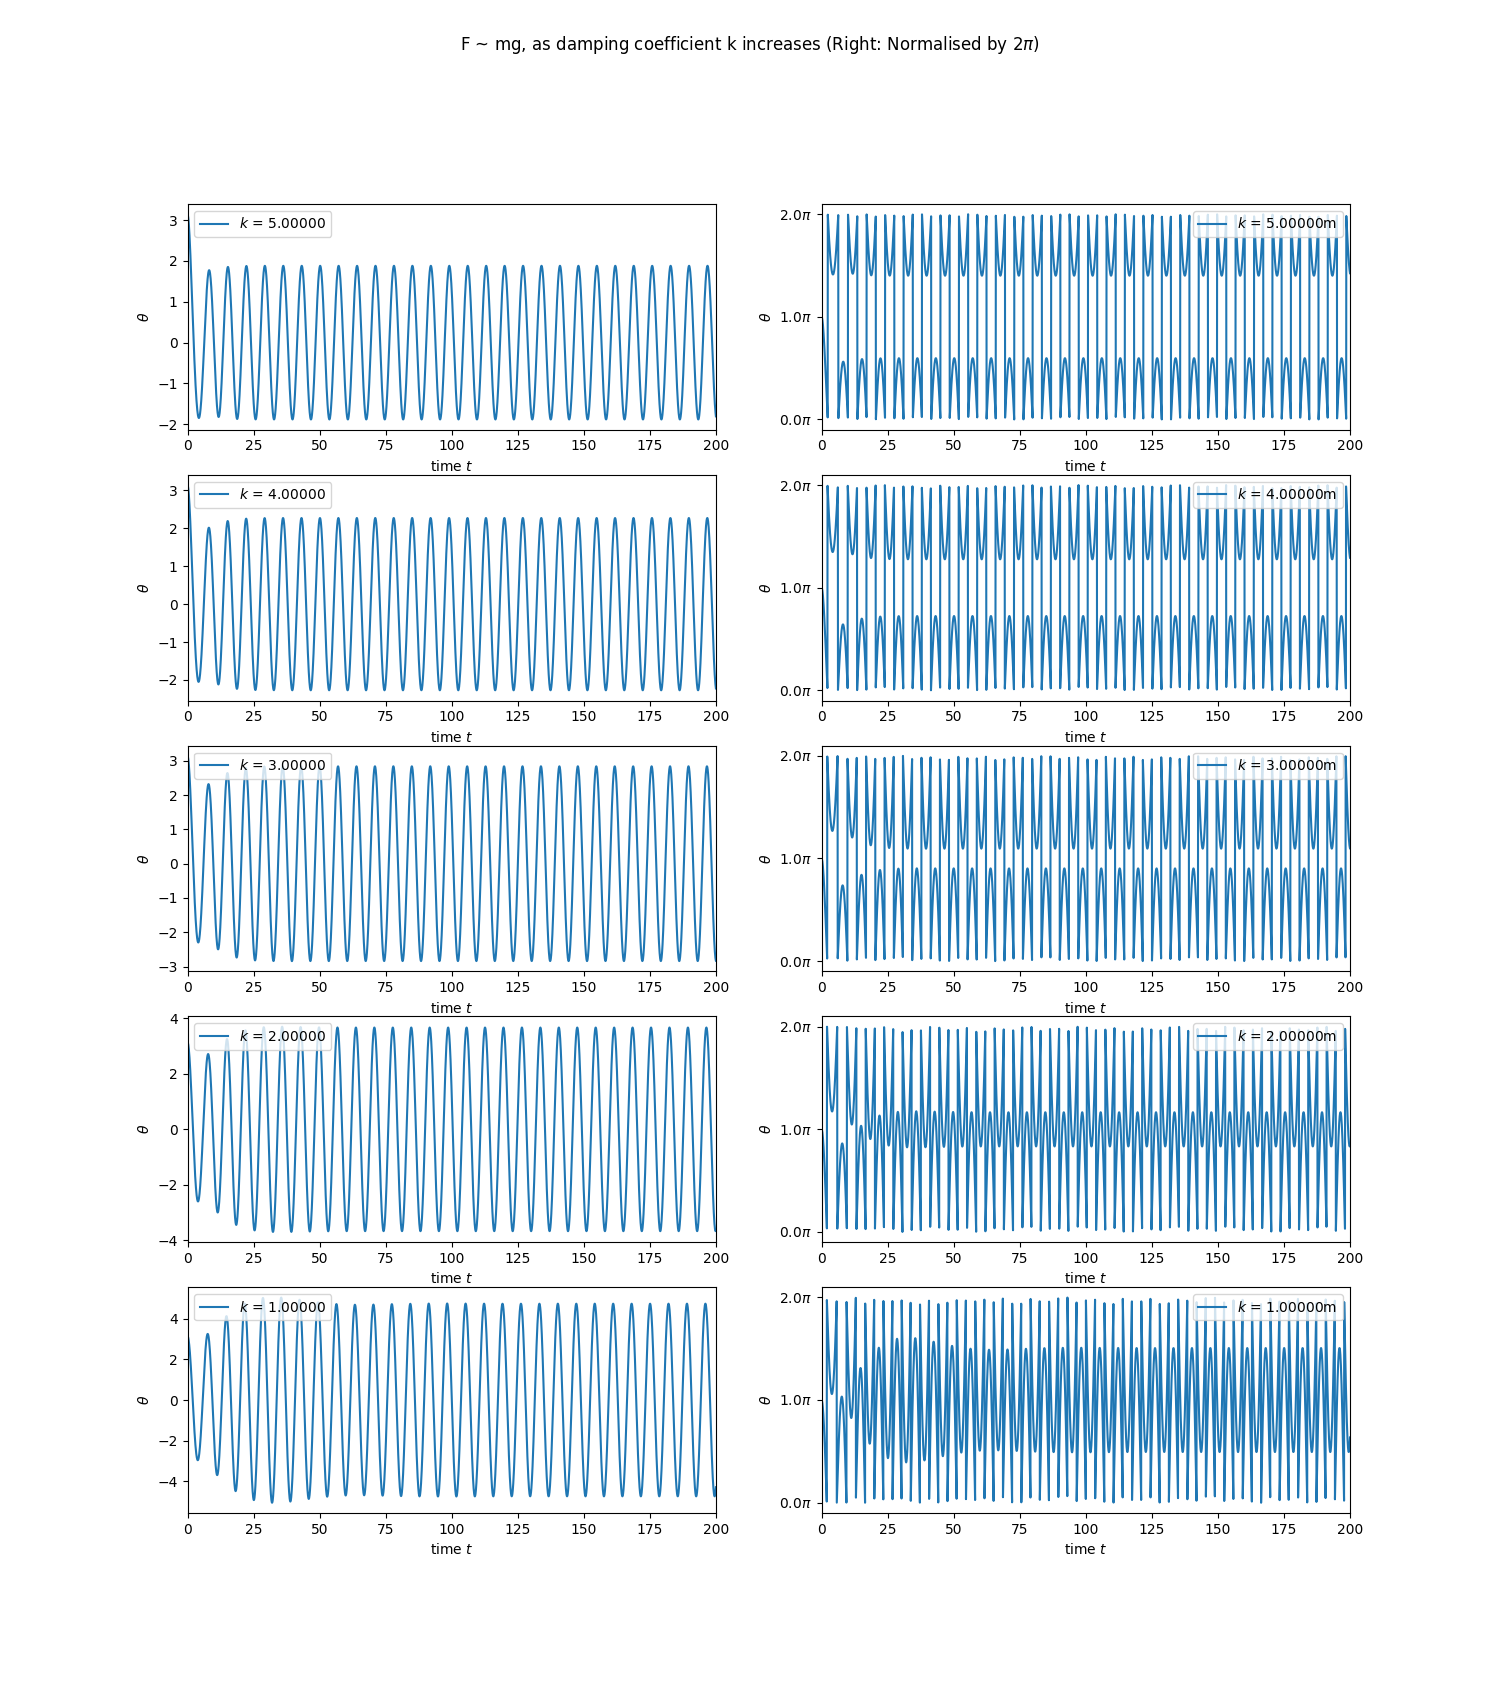
\includegraphics[width = \columnwidth]{Projects/ForcedSimplePendulum/Plots/F~mg as damping coefficient k increases from 5 to 1 (med).png}
    \caption{$F \sim{mg}$ for $k = 5$ to $k = 1$ (200 time steps)}
    \label{k 5 to 1 med}
\end{figure}

\begin{figure}
    \centering
    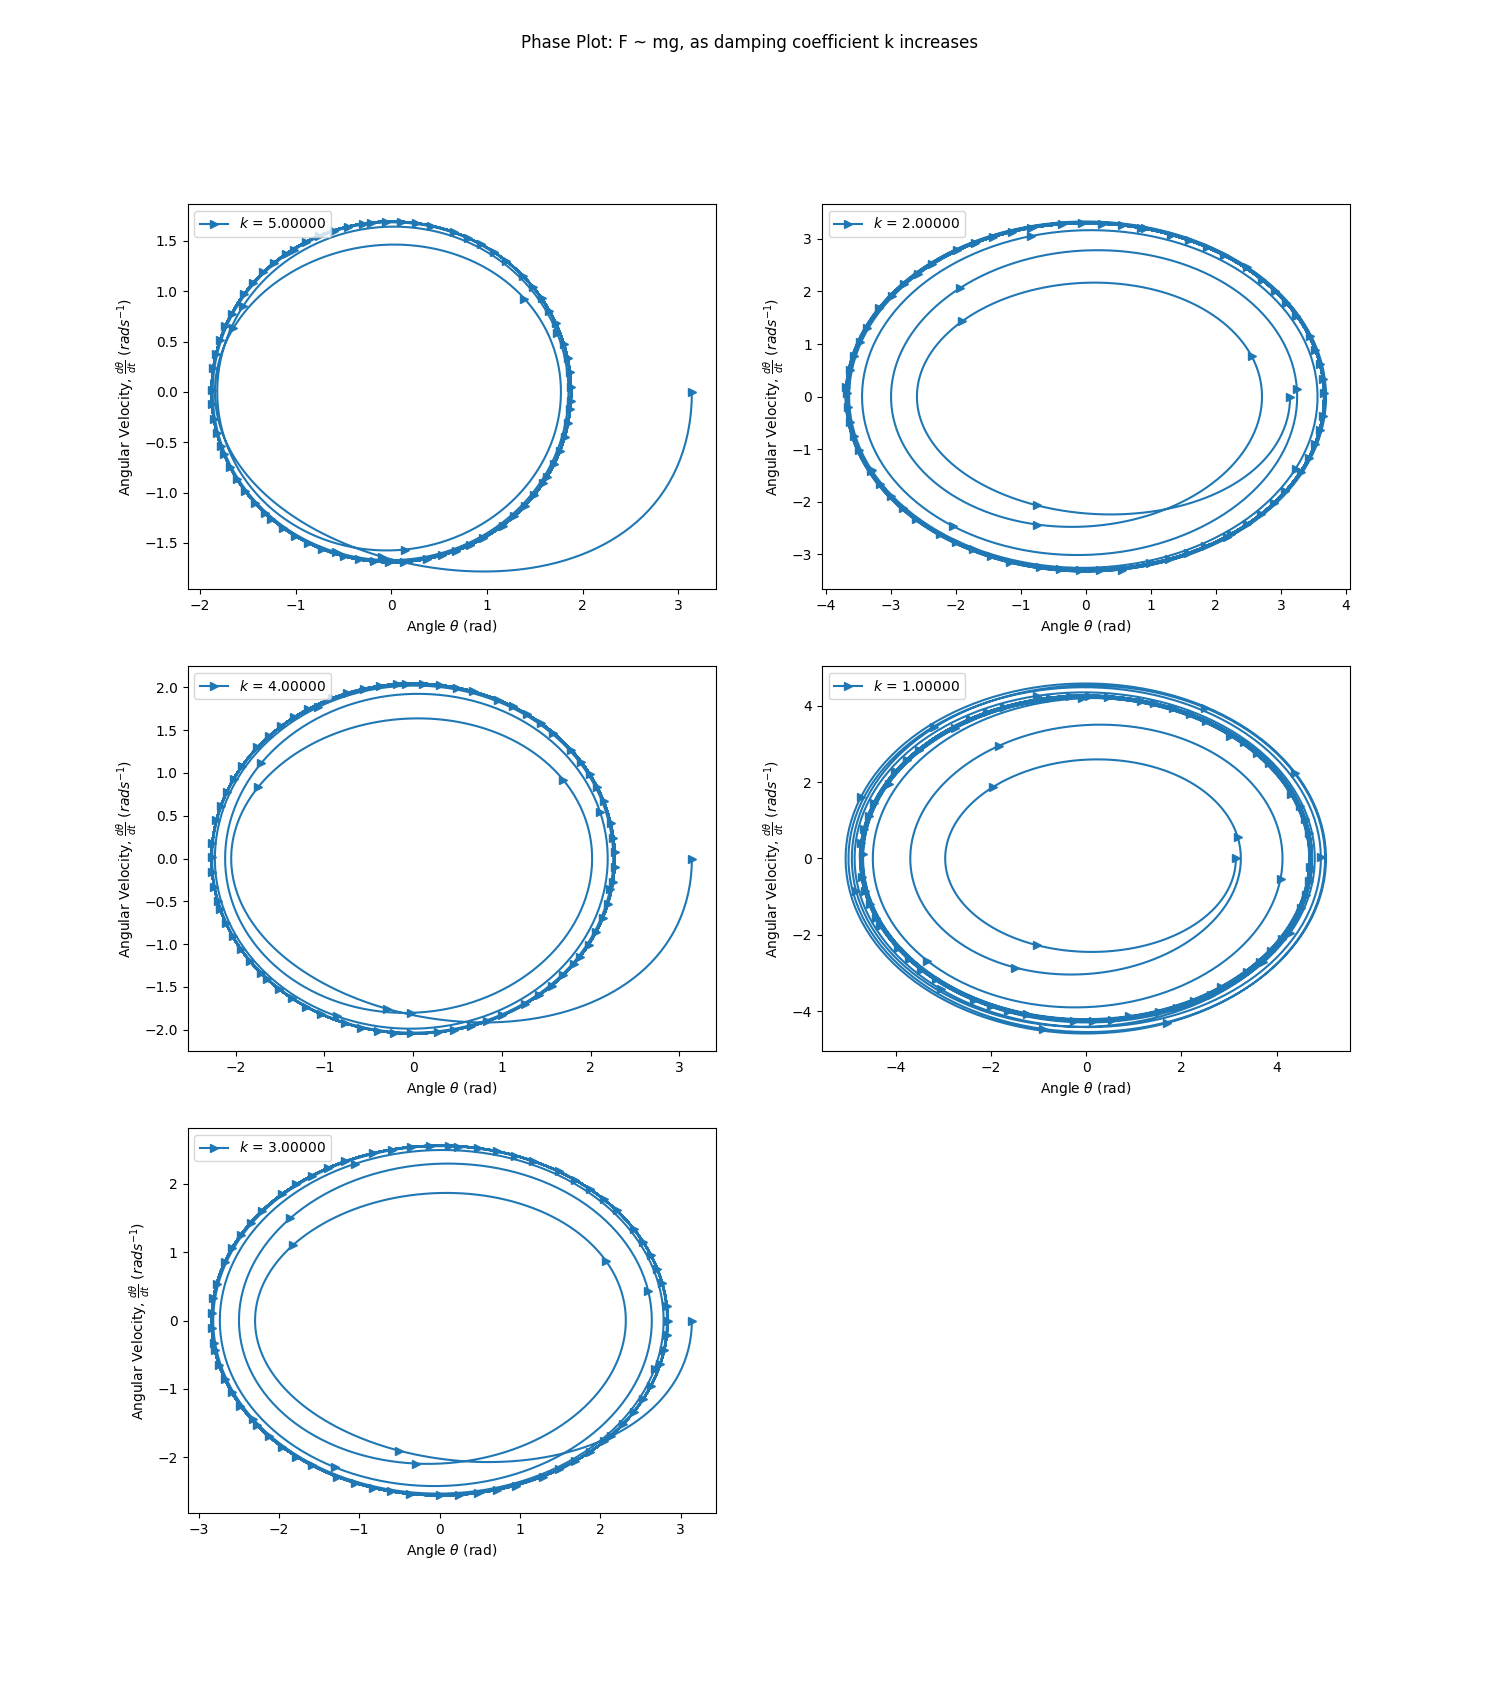
\includegraphics[width = \columnwidth]{Projects/ForcedSimplePendulum/Plots/Phase plot of F~mg as damping coefficient k increases from 5 to 1 (med).png}
    \caption{Phase plot of $F \sim{mg}$ for $k = 5$ to $k = 1$ (200 time steps)}
    \label{Phase plot of k 5 to 1 med}
\end{figure}

\begin{figure}
    \centering
    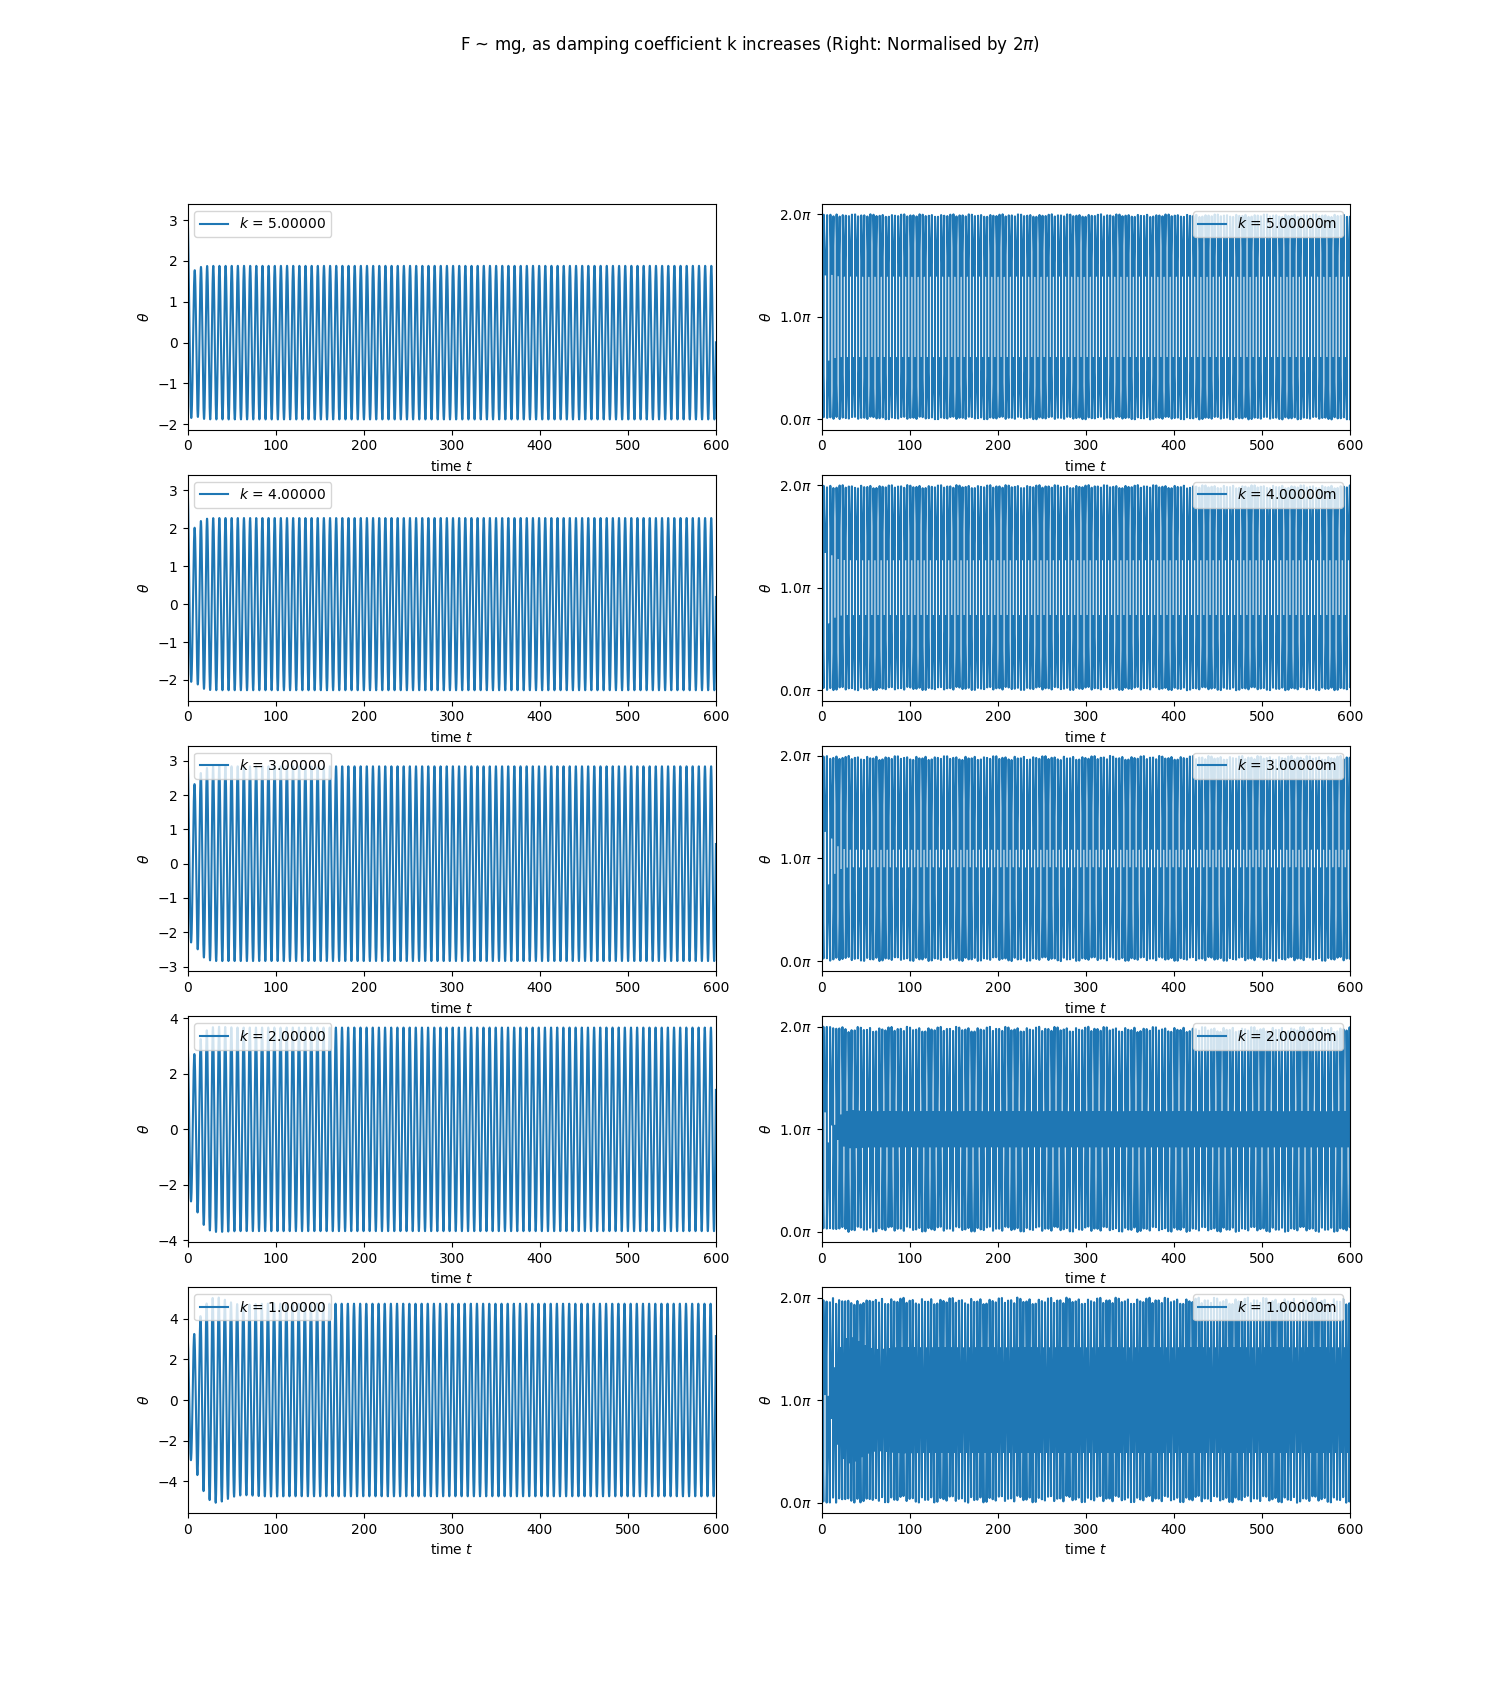
\includegraphics[width = \columnwidth]{Projects/ForcedSimplePendulum/Plots/F~mg as damping coefficient k increases from 5 to 1 (long).png}
    \caption{$F \sim{mg}$ for $k = 5$ to $k = 1$ (600 time steps)}
    \label{k 5 to 1 long}
\end{figure}

\begin{figure}
    \centering
    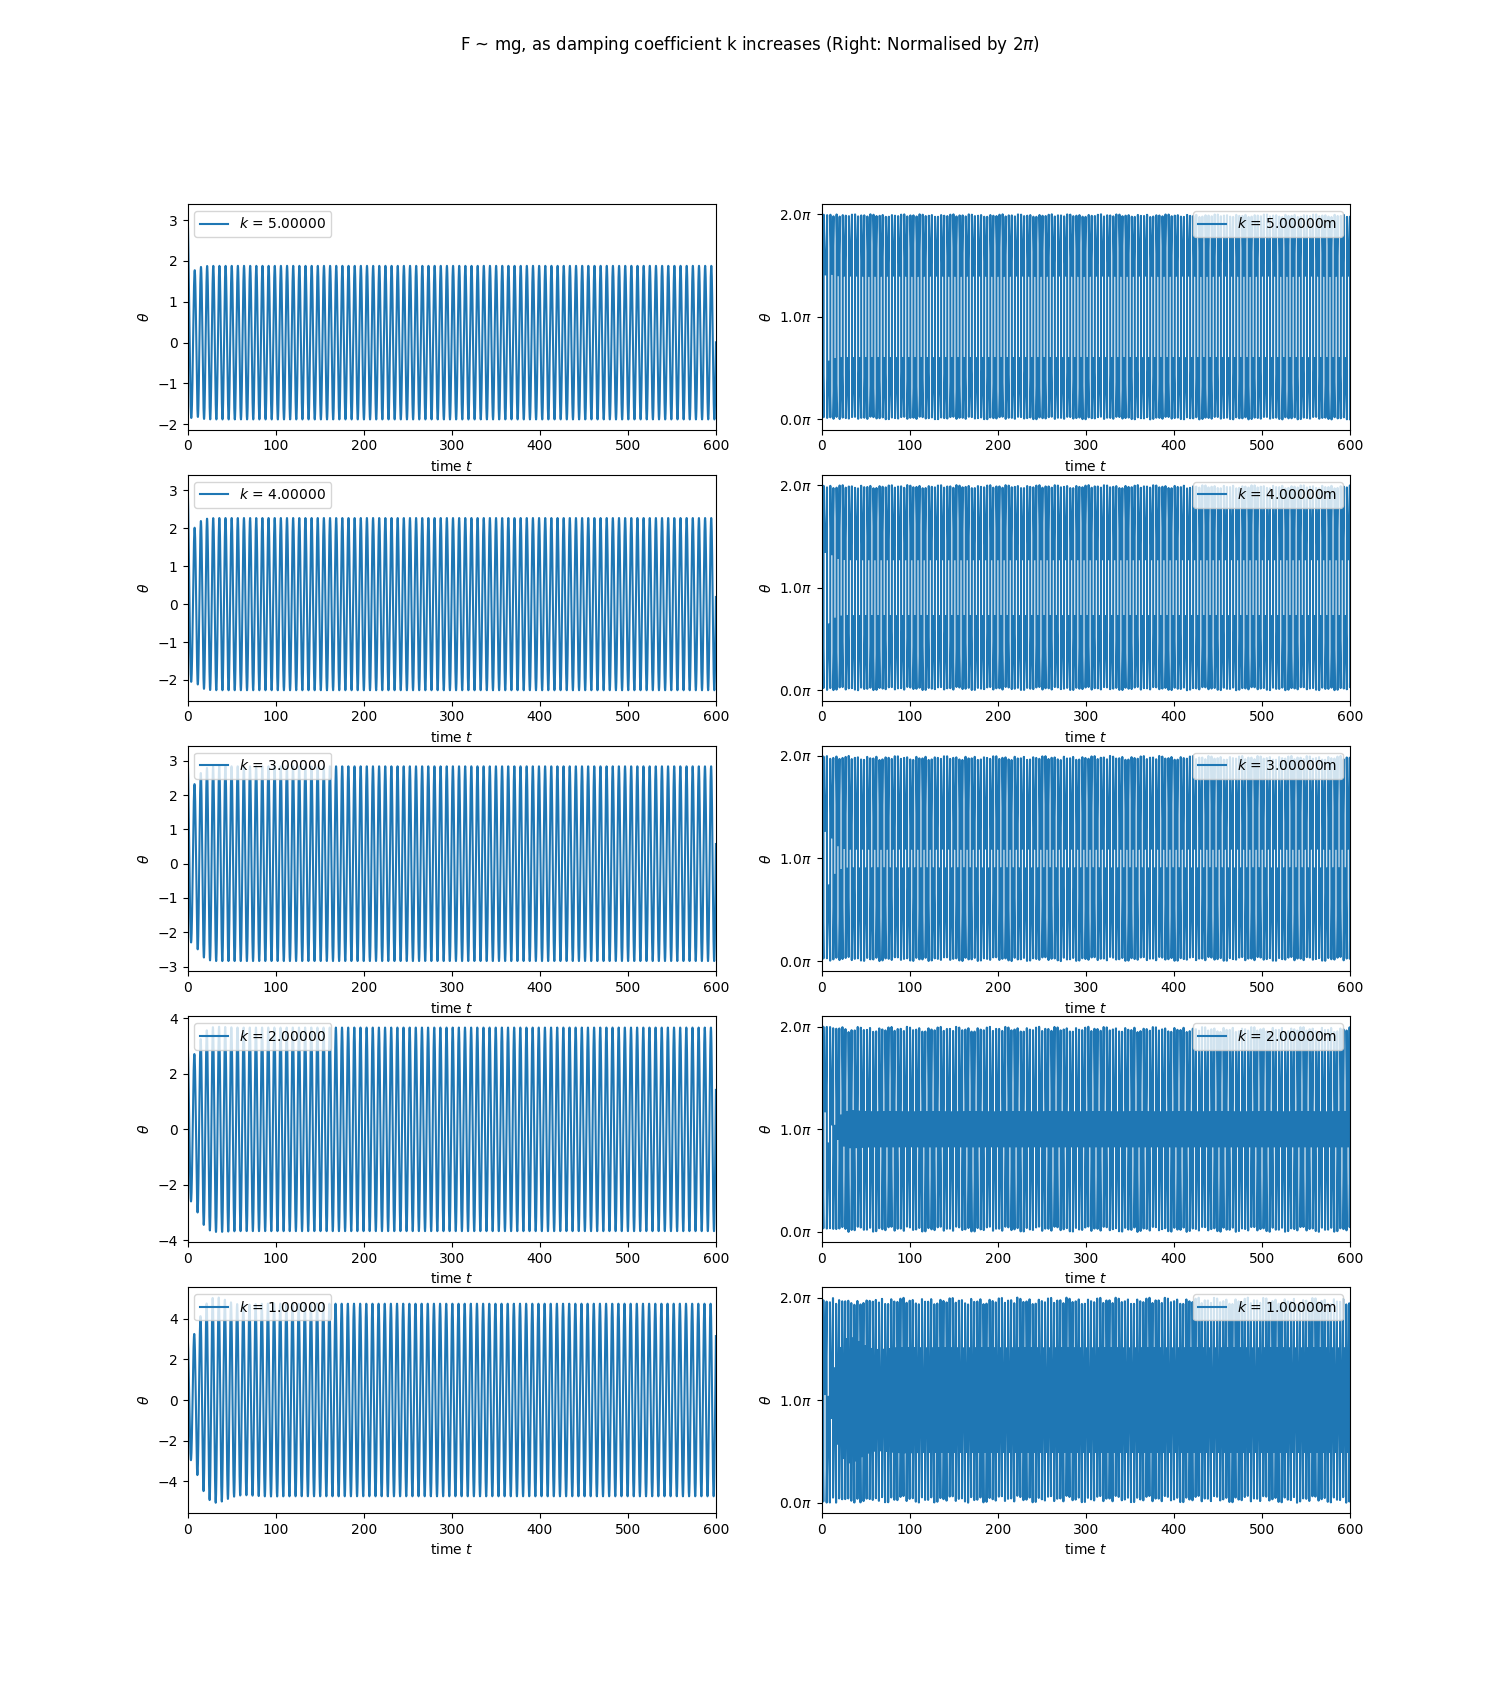
\includegraphics[width = \columnwidth]{Projects/ForcedSimplePendulum/Plots/F~mg as damping coefficient k increases from 5 to 1 (long).png}
    \caption{Phase plot of $F \sim{mg}$ for $k = 5$ to $k = 1$ (600 time steps)}
    \label{Phase plot of k 5 to 1 long}
\end{figure}

Something was happening in that range of $k = 5$ to $k = 1$, so I investigated where k goes from 1 to 0.1.
\begin{figure}
    \centering
    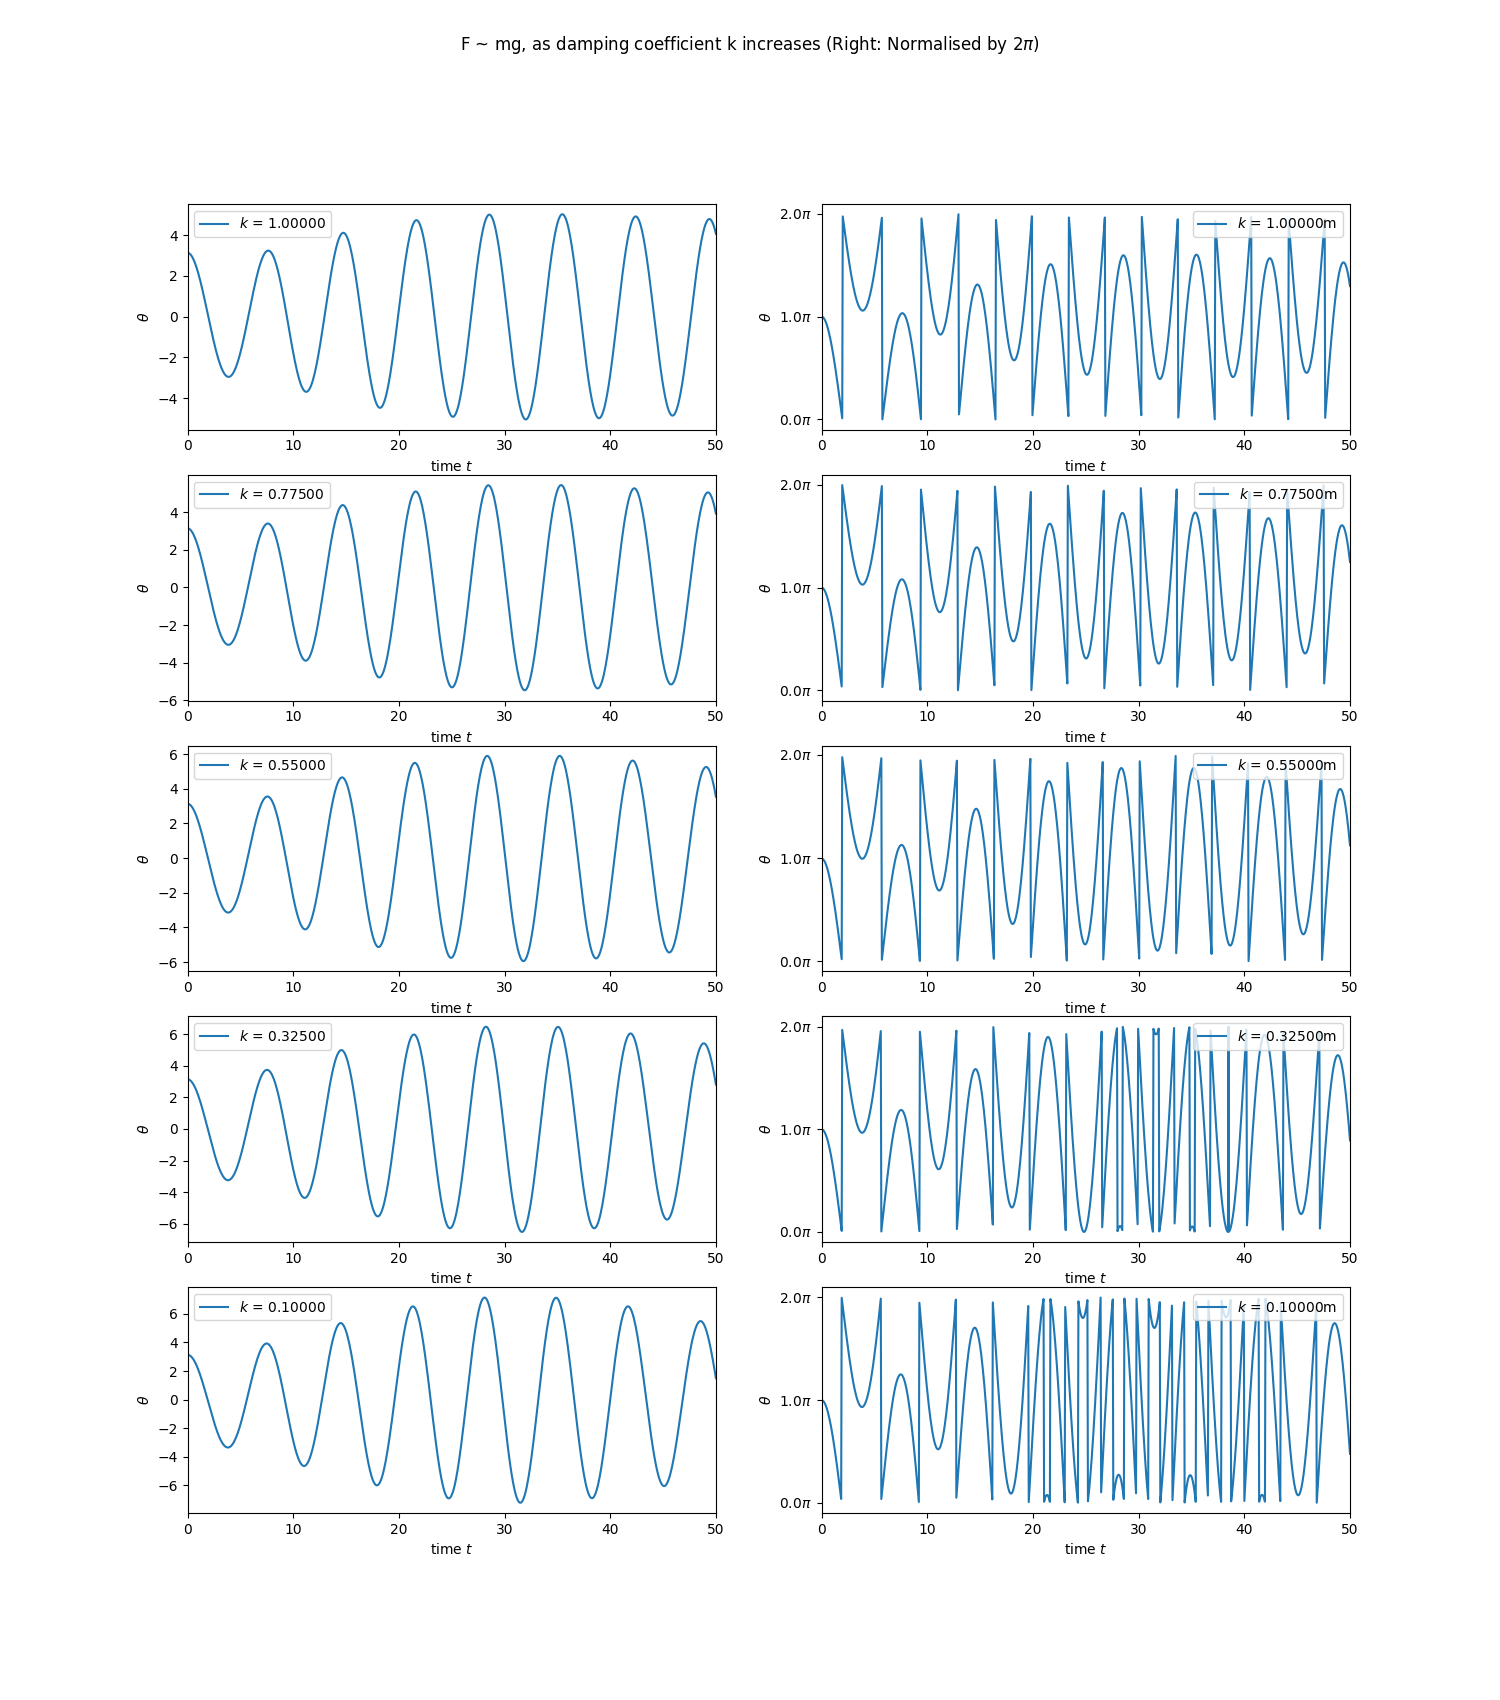
\includegraphics[width = \columnwidth]{Projects/ForcedSimplePendulum/Plots/F~mg as damping coefficient k increases from 1 to 0.1.png}
    \caption{$F \sim{mg}$ for $k = 1$ to $k = 0.1$.}
    \label{k 1 to 0.1}
\end{figure}

\begin{figure}
    \centering
    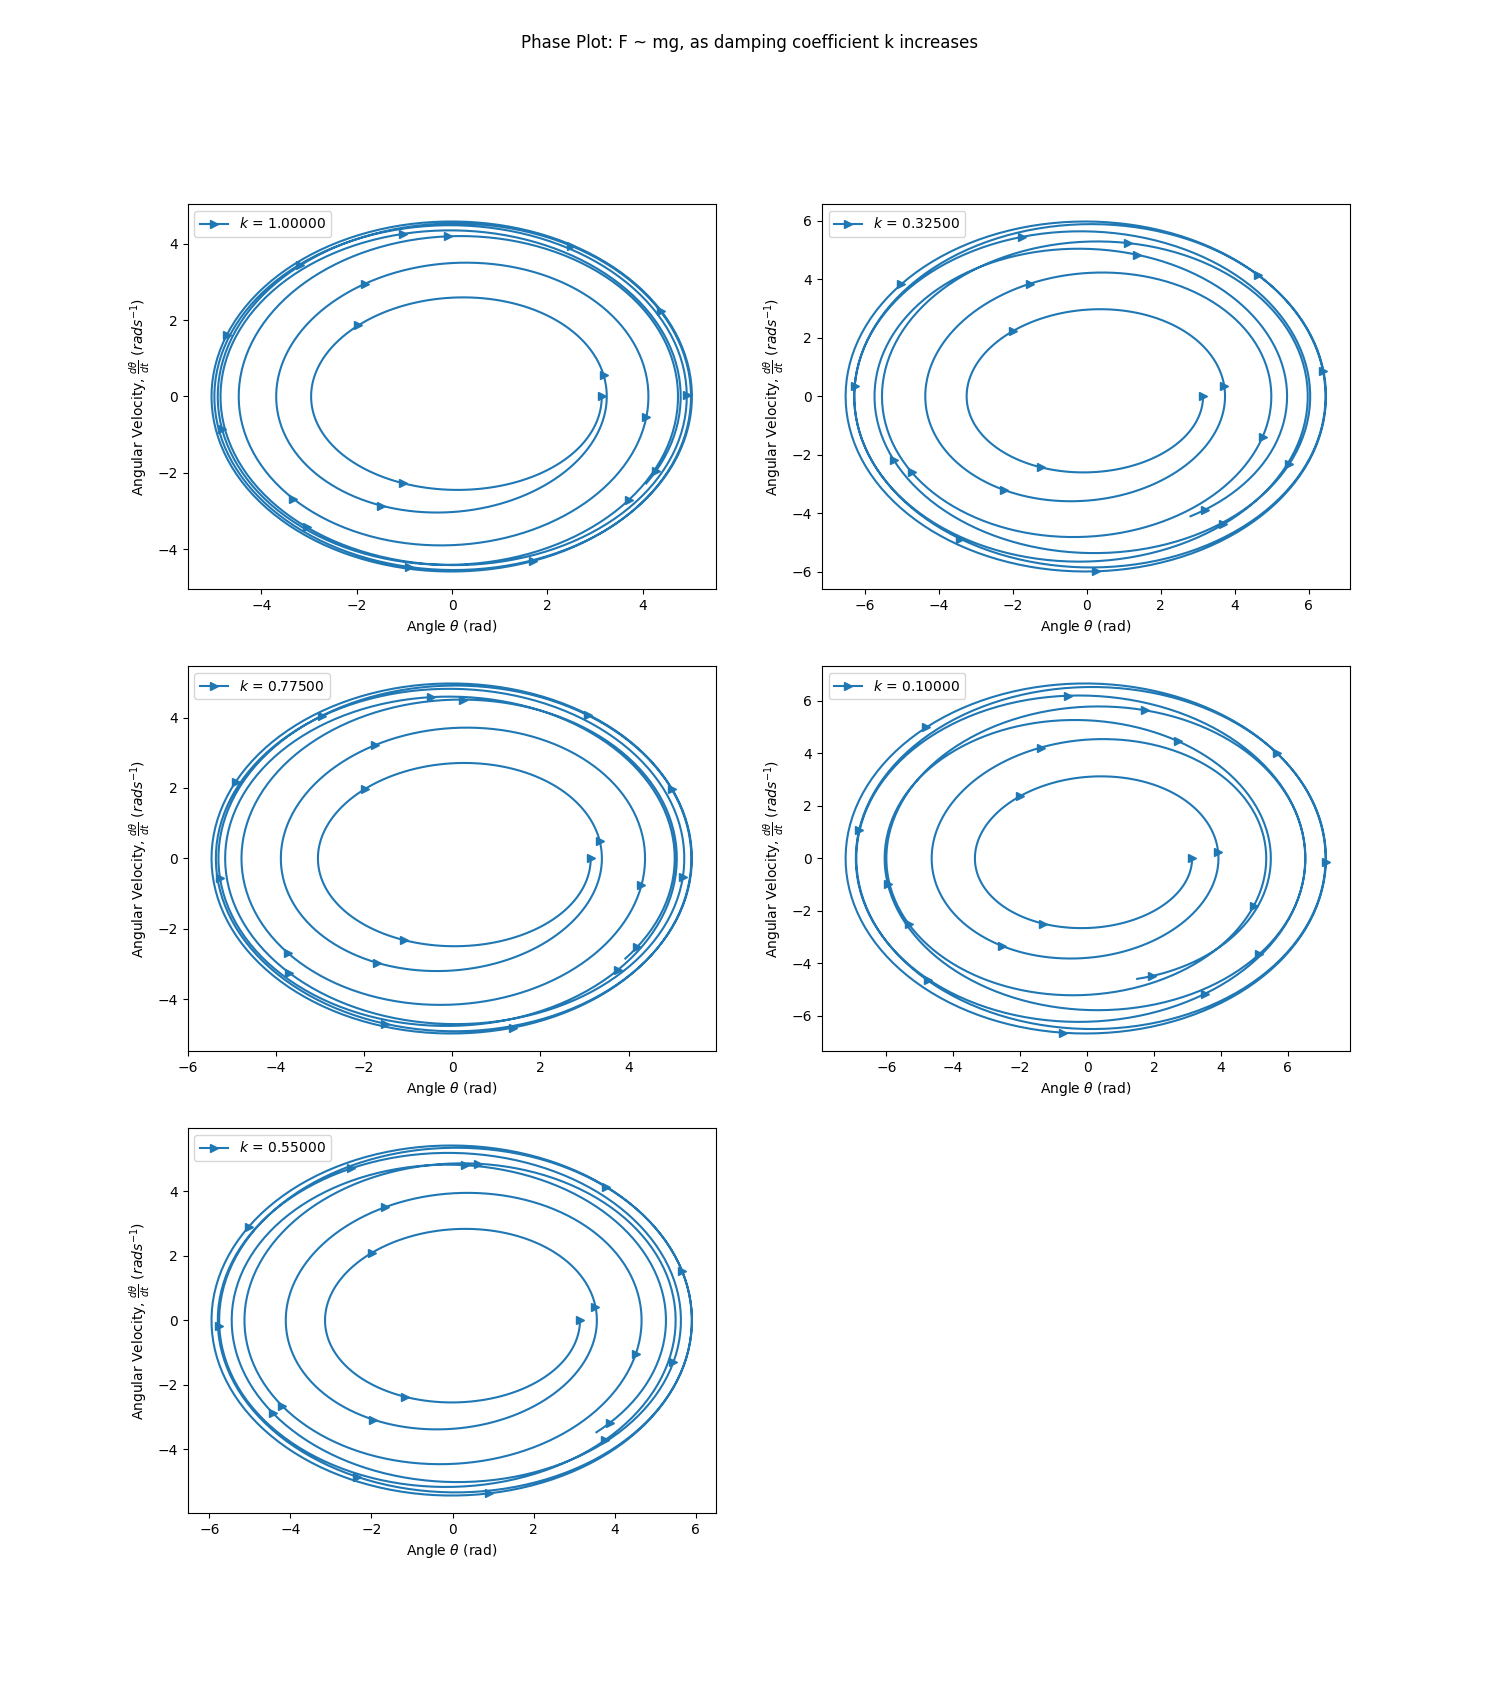
\includegraphics[width = \columnwidth]{Projects/ForcedSimplePendulum/Plots/Phase plot of F~mg as damping coefficient k increases from 1 to 0.1.png}
    \caption{Phase plot of $F \sim{mg}$ for $k = 1$ to $k = 0.1$.}
    \label{Phase plot of k 1 to 0.1}
\end{figure}

\begin{figure}
    \centering
    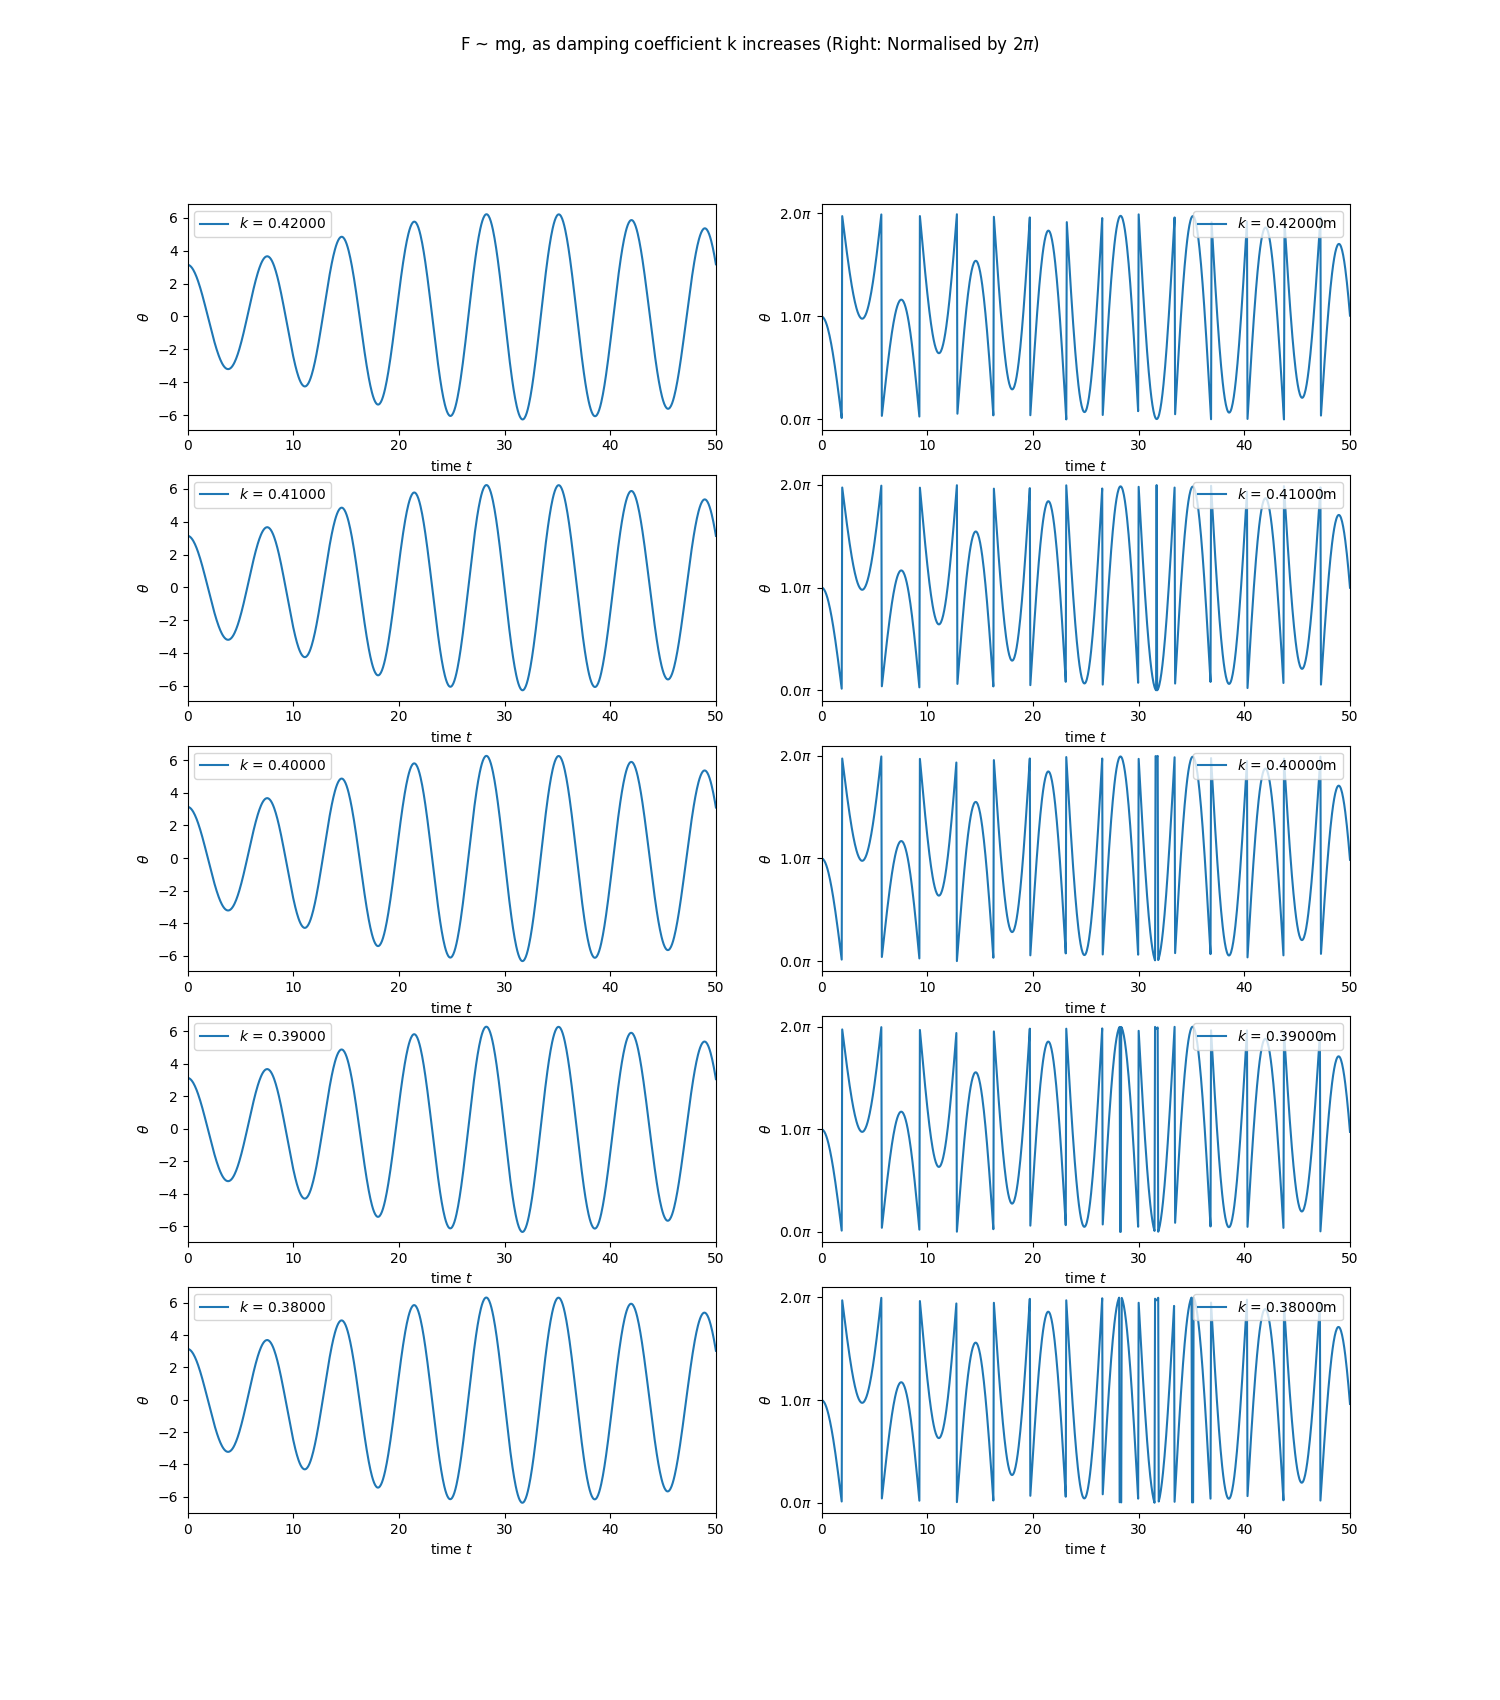
\includegraphics[width = \columnwidth]{Projects/ForcedSimplePendulum/Plots/F~mg as damping coefficient k increases from 0.42 to 0.38.png}
    \caption{$F \sim{mg}$ for $k = 0.42$ to $k = 0.38$.}
    \label{k 0.42 to 0.38}
\end{figure}

\begin{figure}
    \centering
    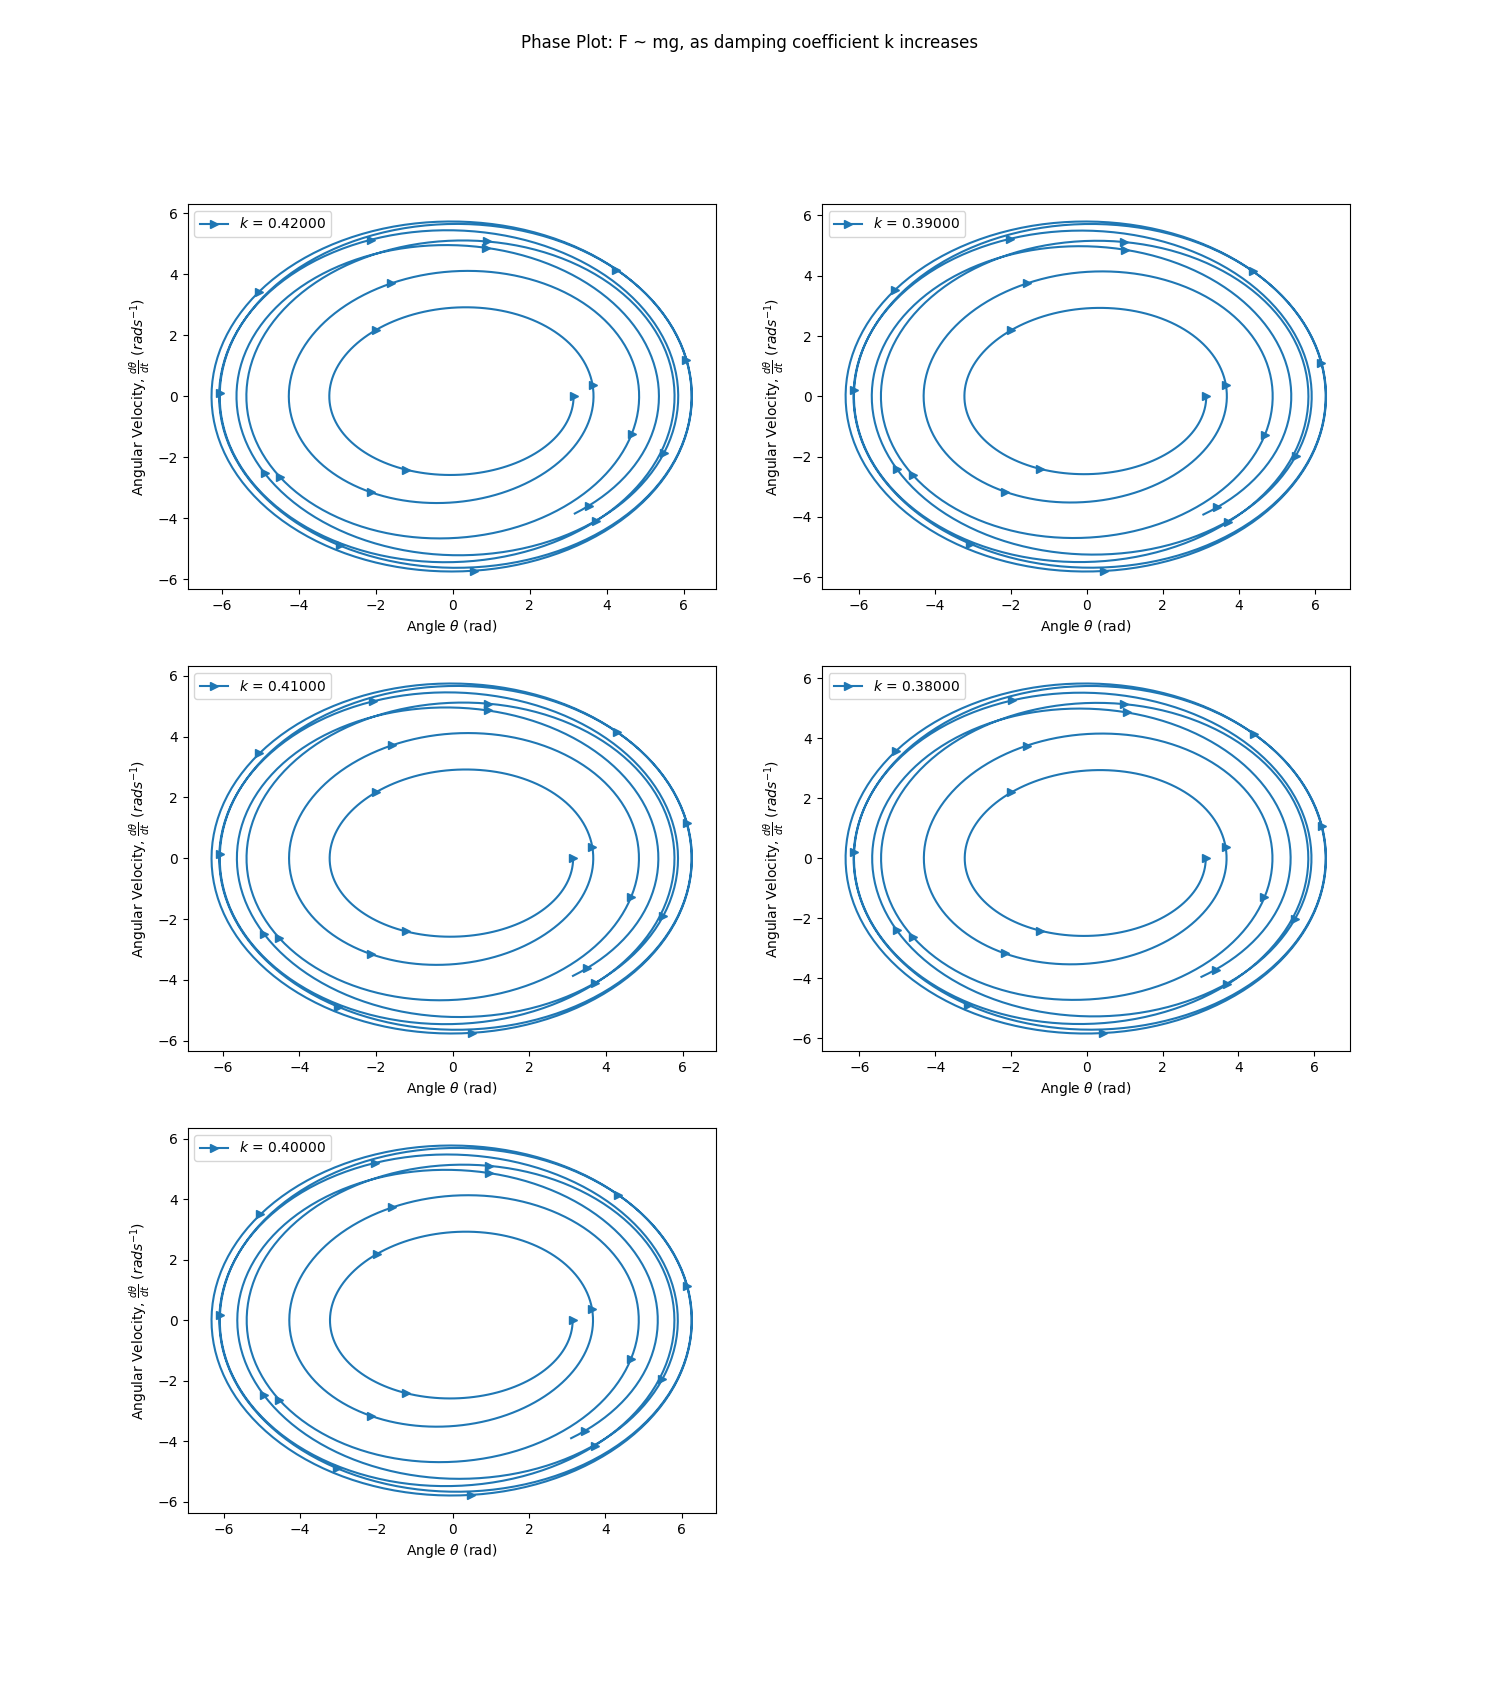
\includegraphics[width = \columnwidth]{Projects/ForcedSimplePendulum/Plots/Phase plot of F~mg as damping coefficient k increases from 0.42 to 0.38.png}
    \caption{Phase plot of $F \sim{mg}$ for $k = 0.42$ to $k = 0.38$.}
    \label{phase plot of k 0.42 to 0.38}
\end{figure}

\begin{figure}
    \centering
    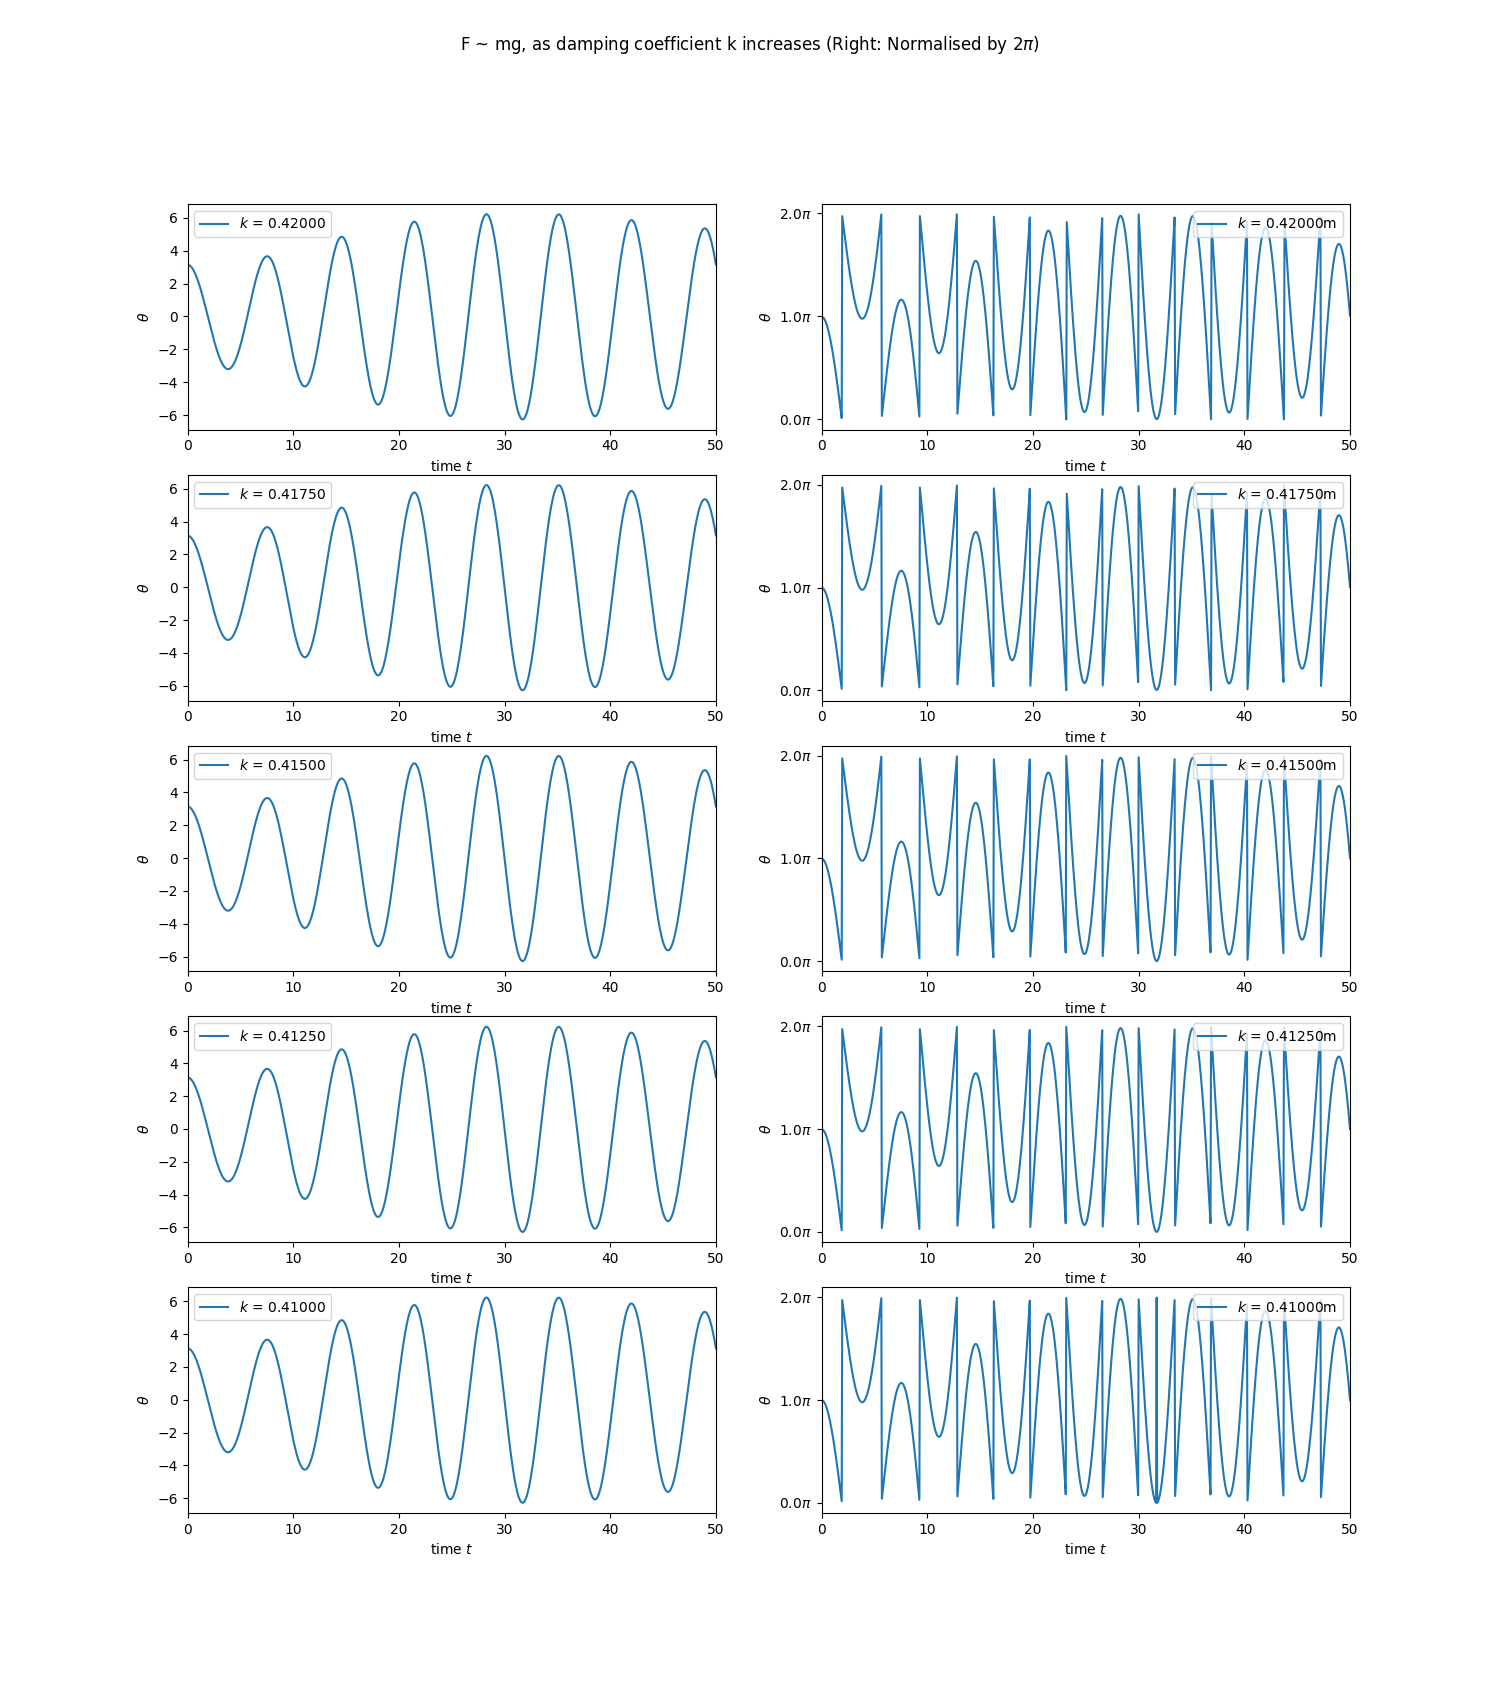
\includegraphics[width = \columnwidth]{Projects/ForcedSimplePendulum/Plots/F~mg as damping coefficient k increases from 0.42 to 0.41.png}
    \caption{$F \sim{mg}$ for $k = 0.42$ to $k = 0.41$.}
    \label{k 0.42 to 0.41}
\end{figure}

\begin{figure}
    \centering
    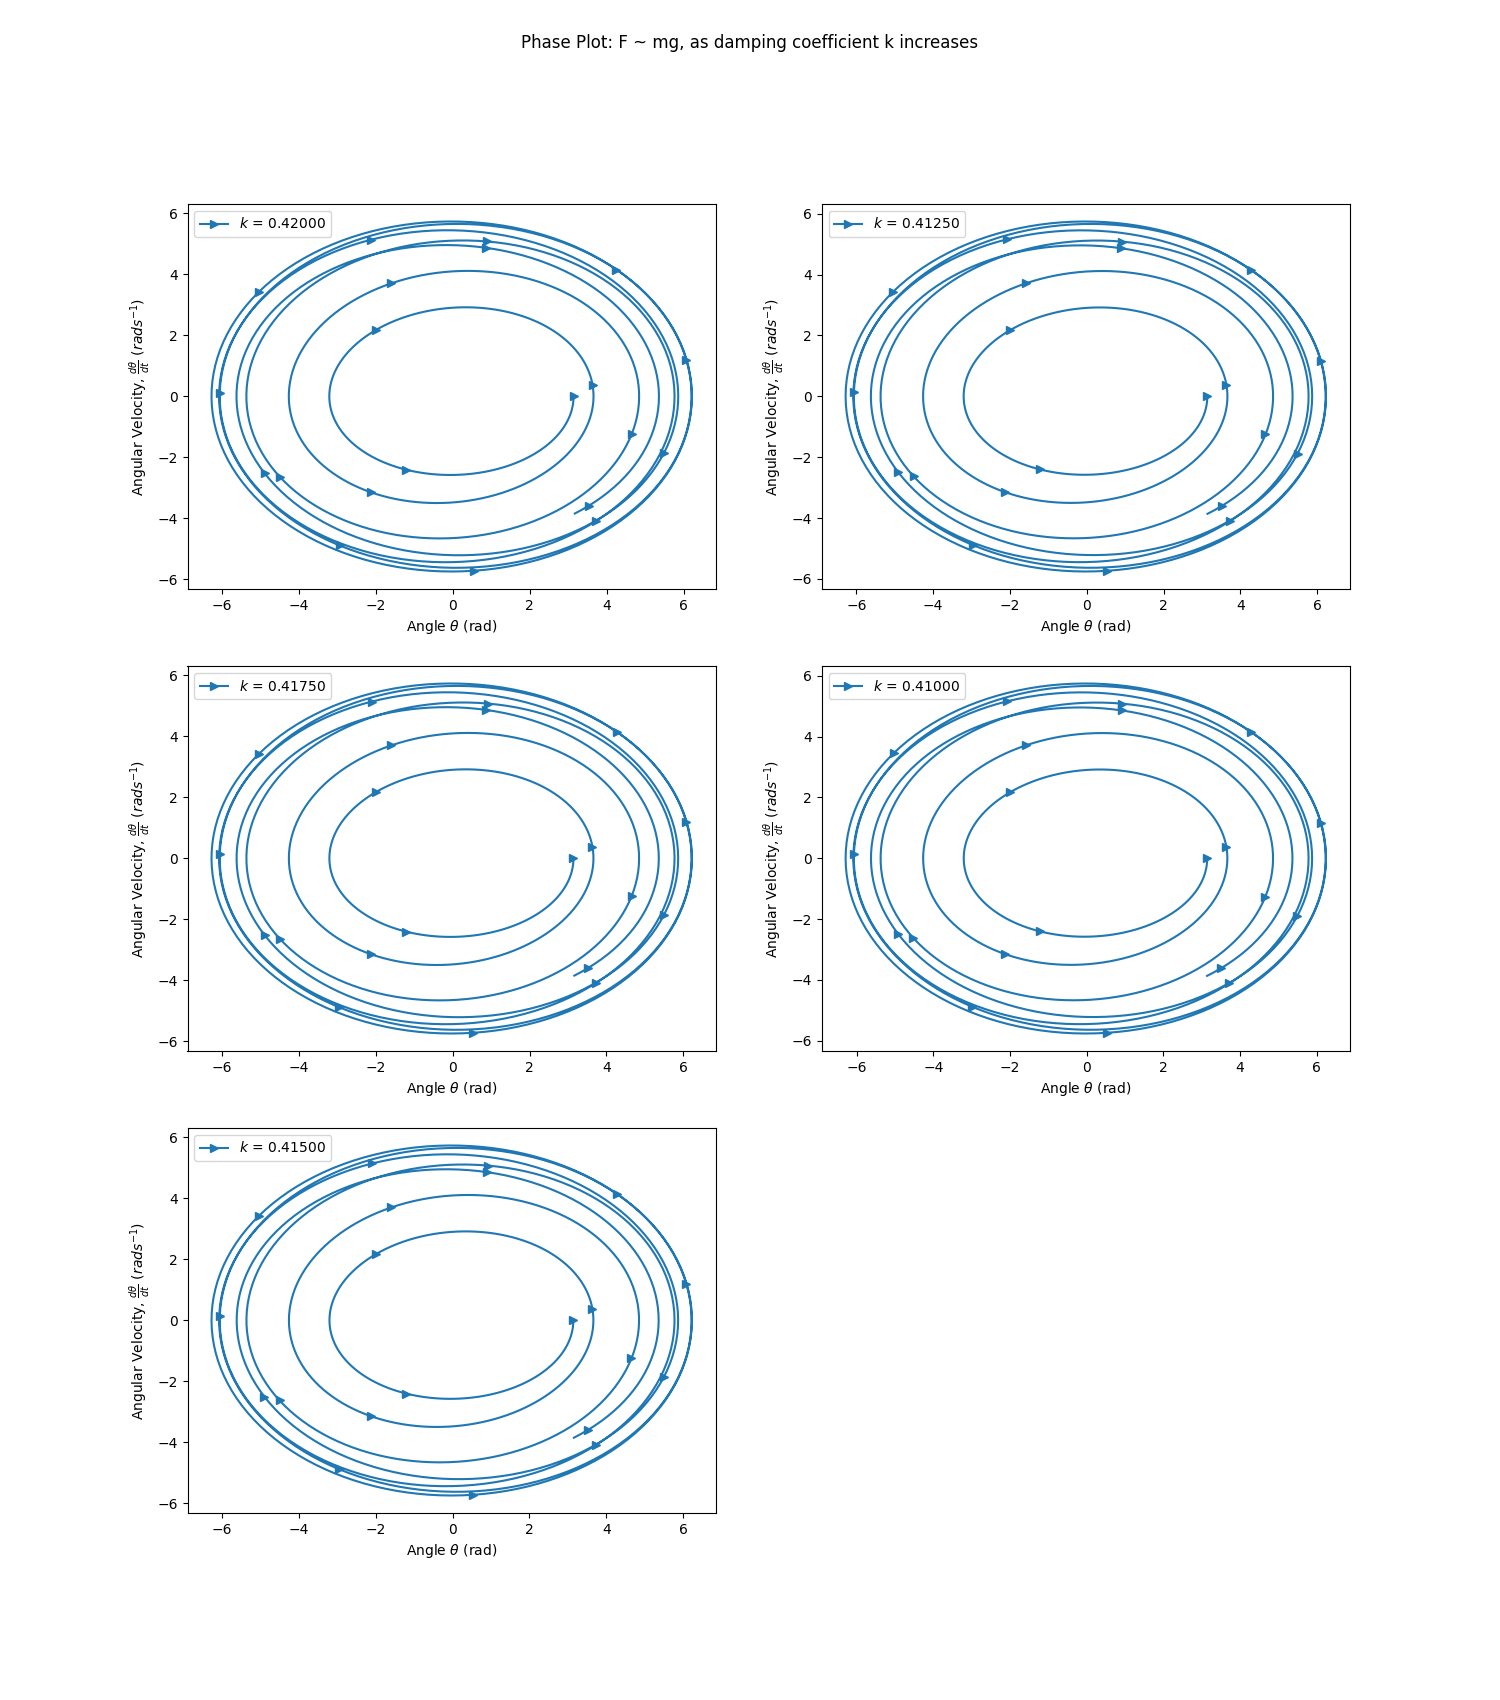
\includegraphics[width = \columnwidth]{Projects/ForcedSimplePendulum/Plots/Phase plot of F~mg as damping coefficient k increases from 0.42 to 0.41.png}
    \caption{Phase plot of $F \sim{mg}$ for $k = 0.42$ to $k = 0.41$.}
    \label{Phase plot of k 0.42 to 0.41}
\end{figure}
\end{document}

\section{Appendix C: Plots for the R-L pendulum}{\label{rlplots}}
\begin{figure}
    \centering
    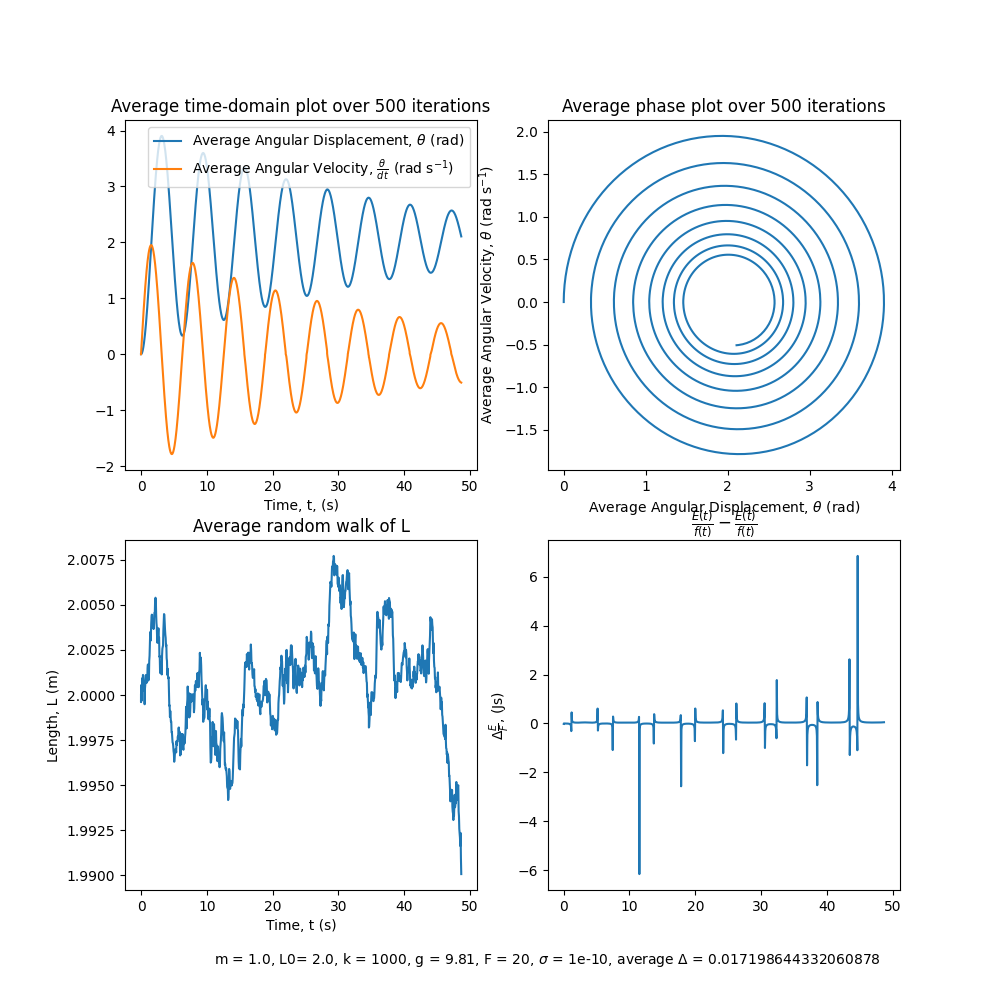
\includegraphics[width = \columnwidth]{Projects/ForcedSimplePendulum/Plots/m = 1.0, L0= 2.0, k = 1000, g = 9.81, F = 20, sigma = 1e-10, run number 0.png}
    \caption{First Iteration.}
    \label{fig:enter-label}
\end{figure}

\begin{figure}
    \centering
    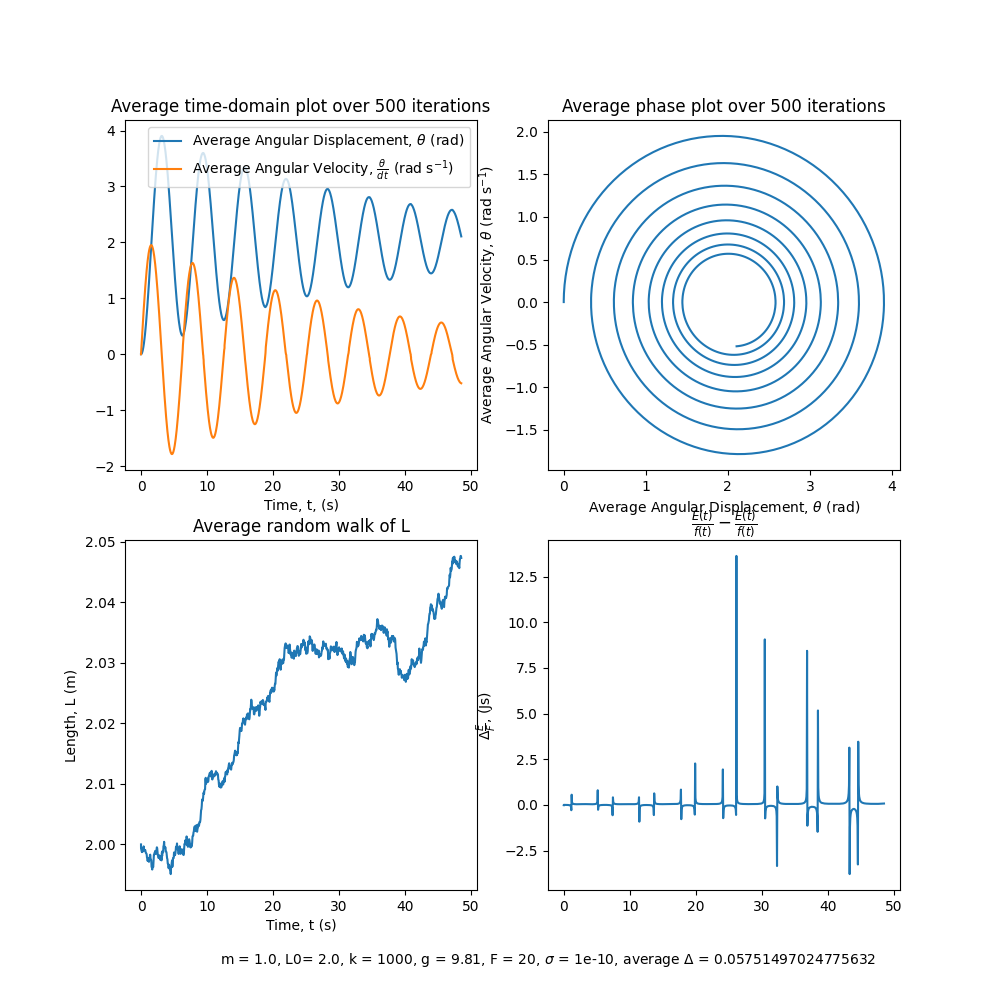
\includegraphics[width = \columnwidth]{Projects/ForcedSimplePendulum/Plots/m = 1.0, L0= 2.0, k = 1000, g = 9.81, F = 20, sigma = 1e-10, run number 1.png}
    \caption{Second Iteration.}
    \label{fig:enter-label}
\end{figure}

\begin{figure}
    \centering
    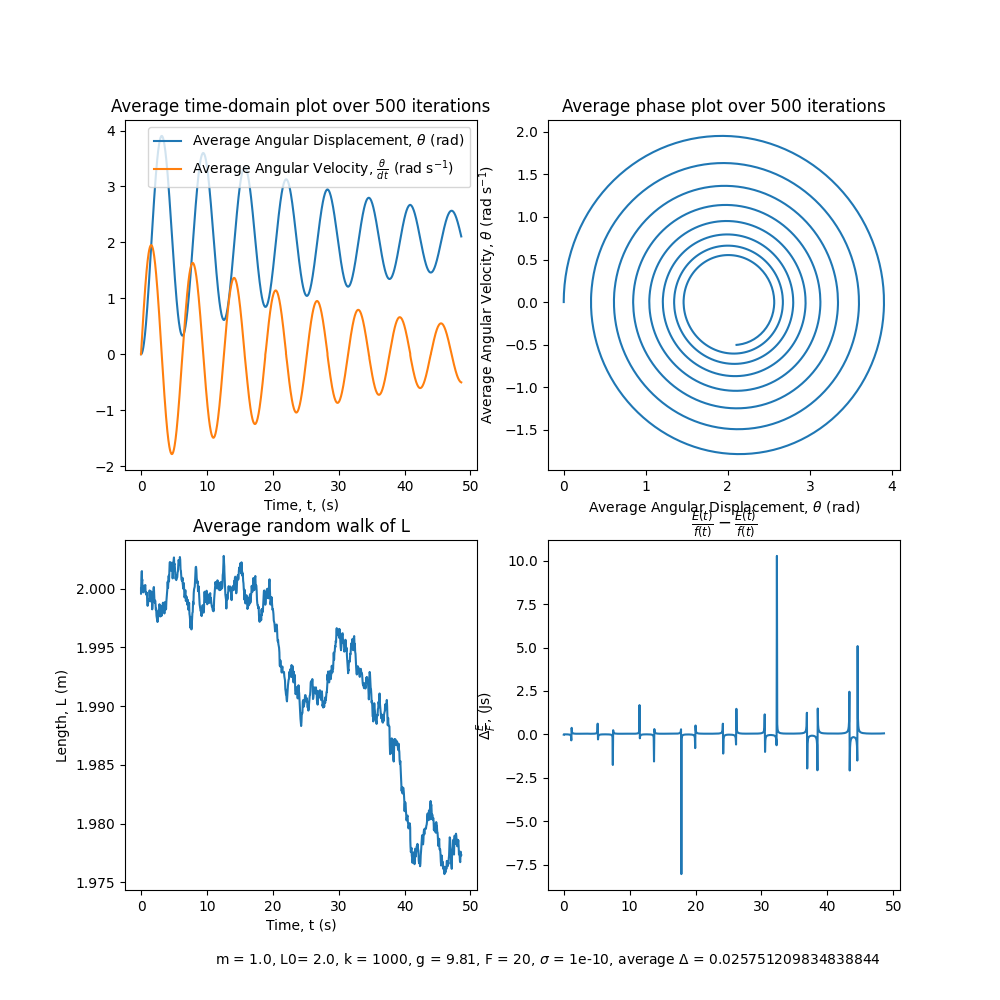
\includegraphics[width = \columnwidth]{Projects/ForcedSimplePendulum/Plots/m = 1.0, L0= 2.0, k = 1000, g = 9.81, F = 20, sigma = 1e-10, run number 2.png}
    \caption{Third Iteration.}
    \label{fig:enter-label}
\end{figure}

\begin{figure}
    \centering
    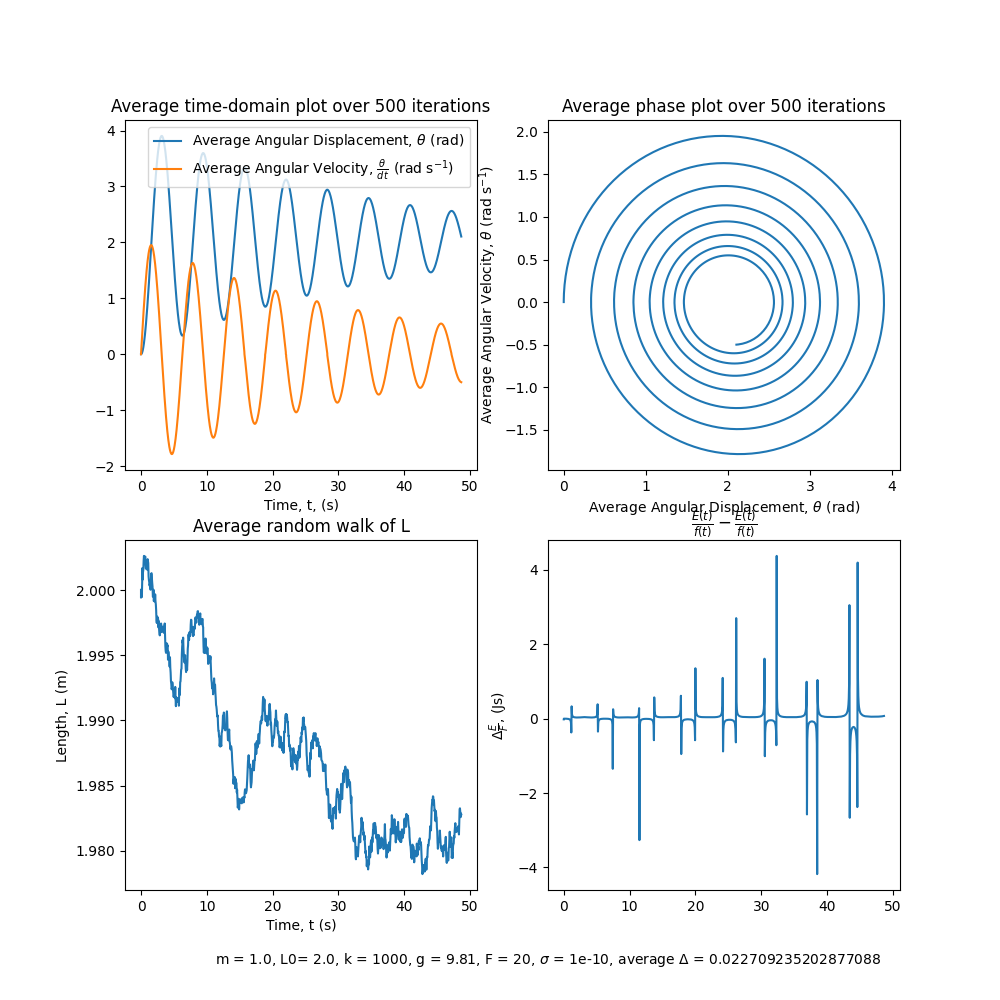
\includegraphics[width = \columnwidth]{Projects/ForcedSimplePendulum/Plots/m = 1.0, L0= 2.0, k = 1000, g = 9.81, F = 20, sigma = 1e-10, run number 3.png}
    \caption{Fourth Iteration.}
    \label{fig:enter-label}
\end{figure}

\begin{figure}
    \centering
    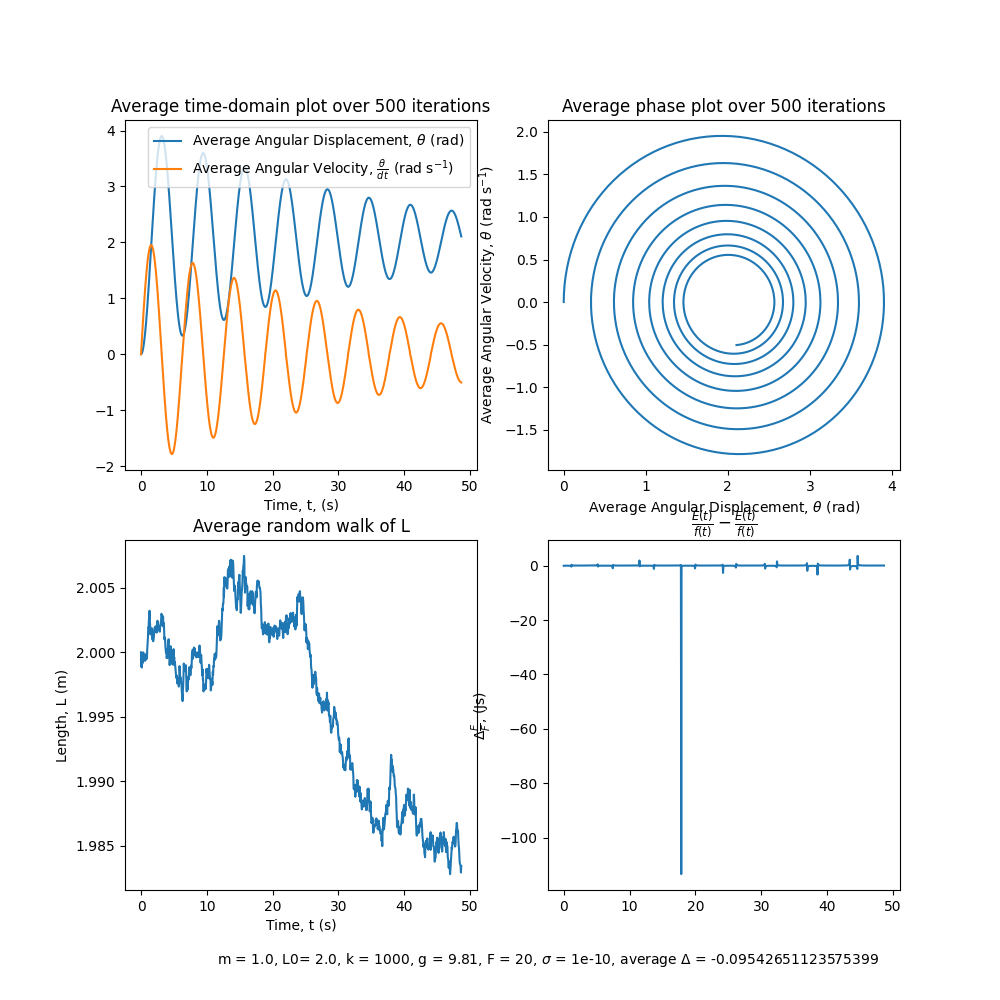
\includegraphics[width = \columnwidth]{Projects/ForcedSimplePendulum/Plots/m = 1.0, L0= 2.0, k = 1000, g = 9.81, F = 20, sigma = 1e-10, run number 4.png}
    \caption{Fifth Iteration.}
    \label{fig:enter-label}
\end{figure}

\begin{figure}
    \centering
    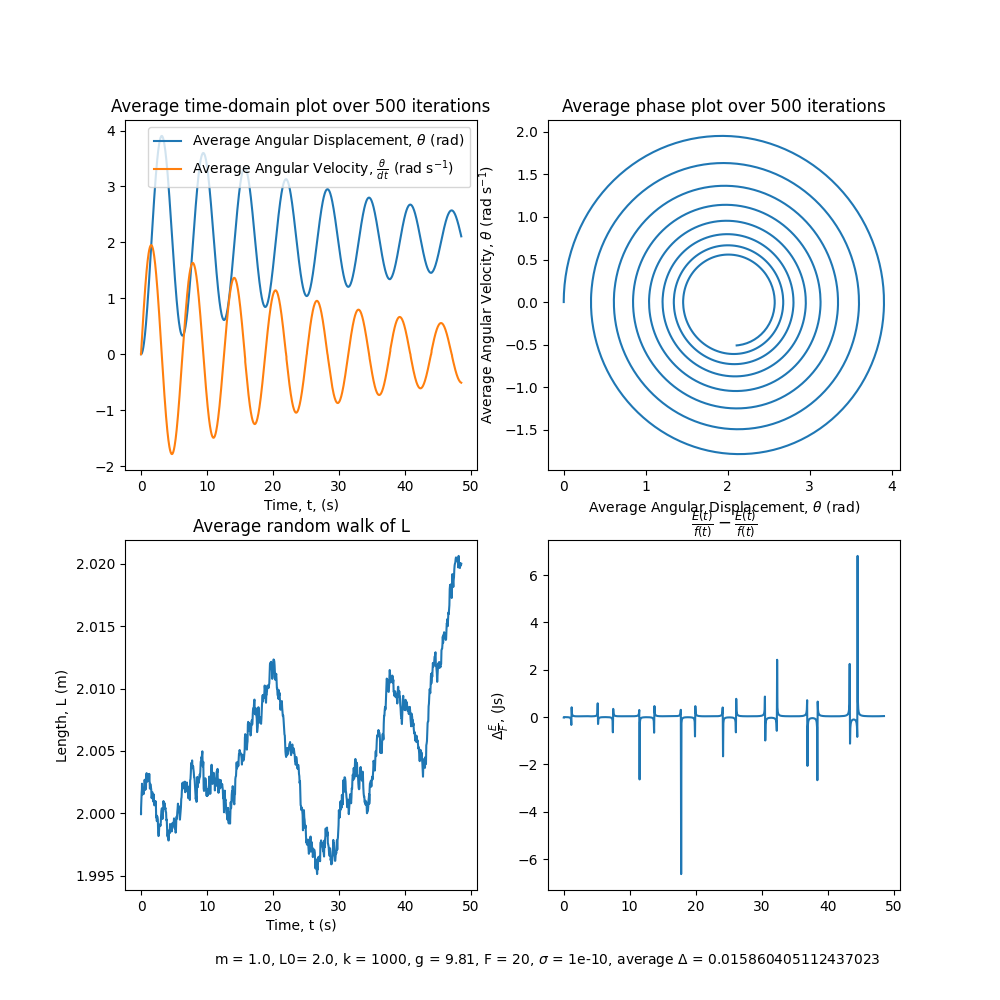
\includegraphics[width = \columnwidth]{Projects/ForcedSimplePendulum/Plots/m = 1.0, L0= 2.0, k = 1000, g = 9.81, F = 20, sigma = 1e-10, run number 5.png}
    \caption{Sixth Iteration.}
    \label{fig:enter-label}
\end{figure}

\begin{figure}
    \centering
    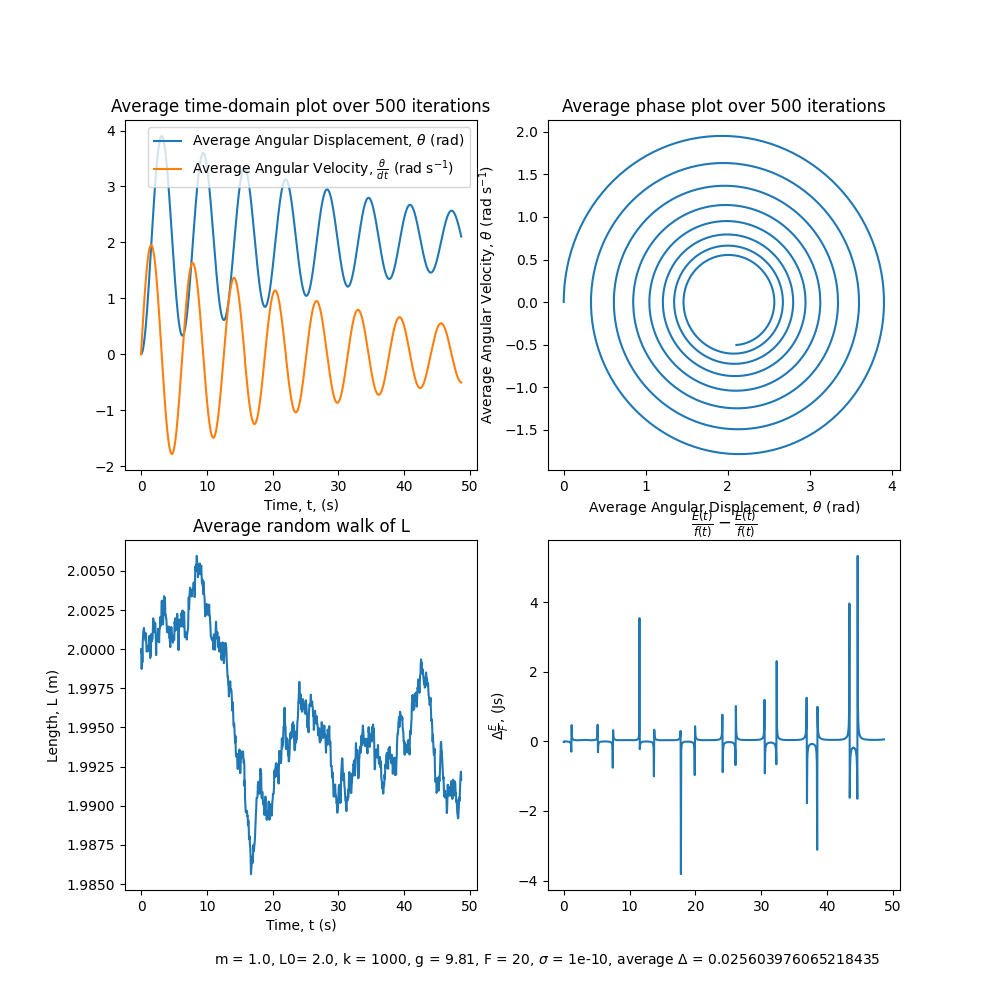
\includegraphics[width = \columnwidth]{Projects/ForcedSimplePendulum/Plots/m = 1.0, L0= 2.0, k = 1000, g = 9.81, F = 20, sigma = 1e-10, run number 6.png}
    \caption{Seventh Iteration.}
    \label{fig:enter-label}
\end{figure}

\begin{figure}
    \centering
    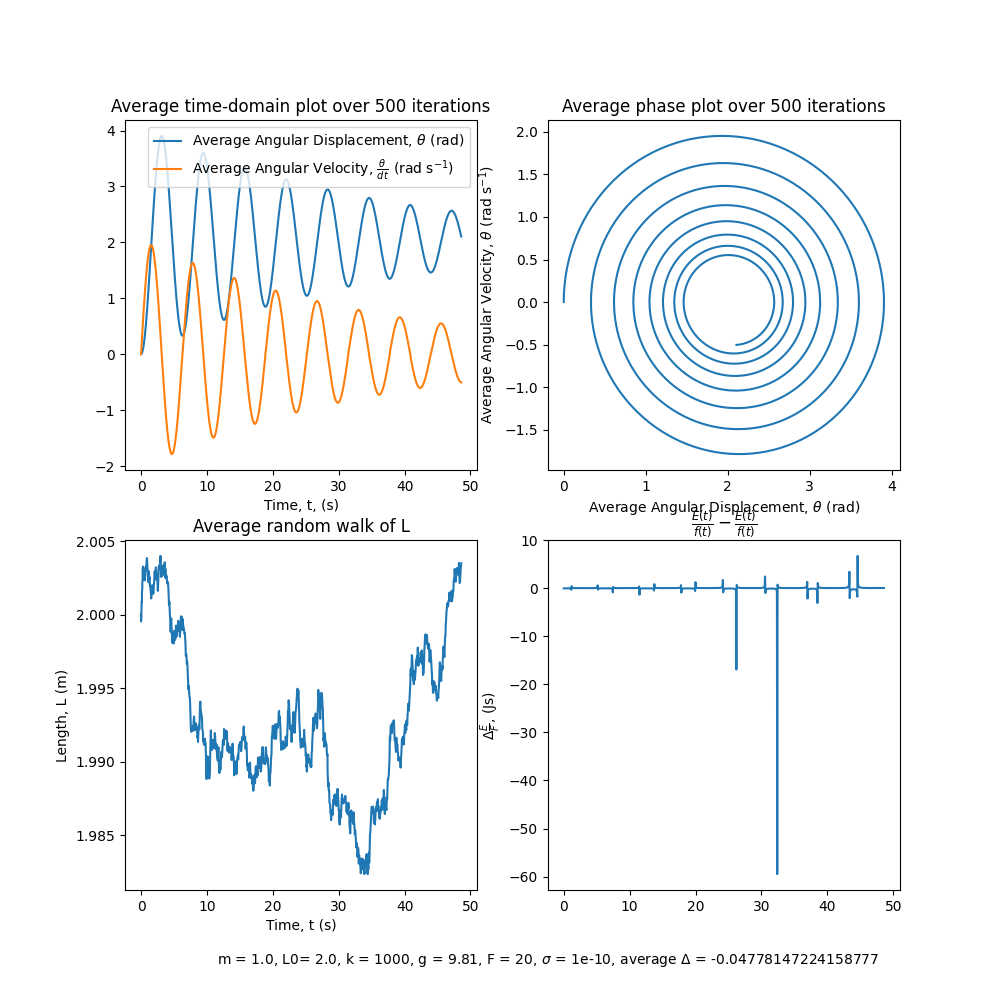
\includegraphics[width = \columnwidth]{Projects/ForcedSimplePendulum/Plots/m = 1.0, L0= 2.0, k = 1000, g = 9.81, F = 20, sigma = 1e-10, run number 7.png}
    \caption{Eighth Iteration.}
    \label{fig:enter-label}
\end{figure}

\begin{figure}
    \centering
    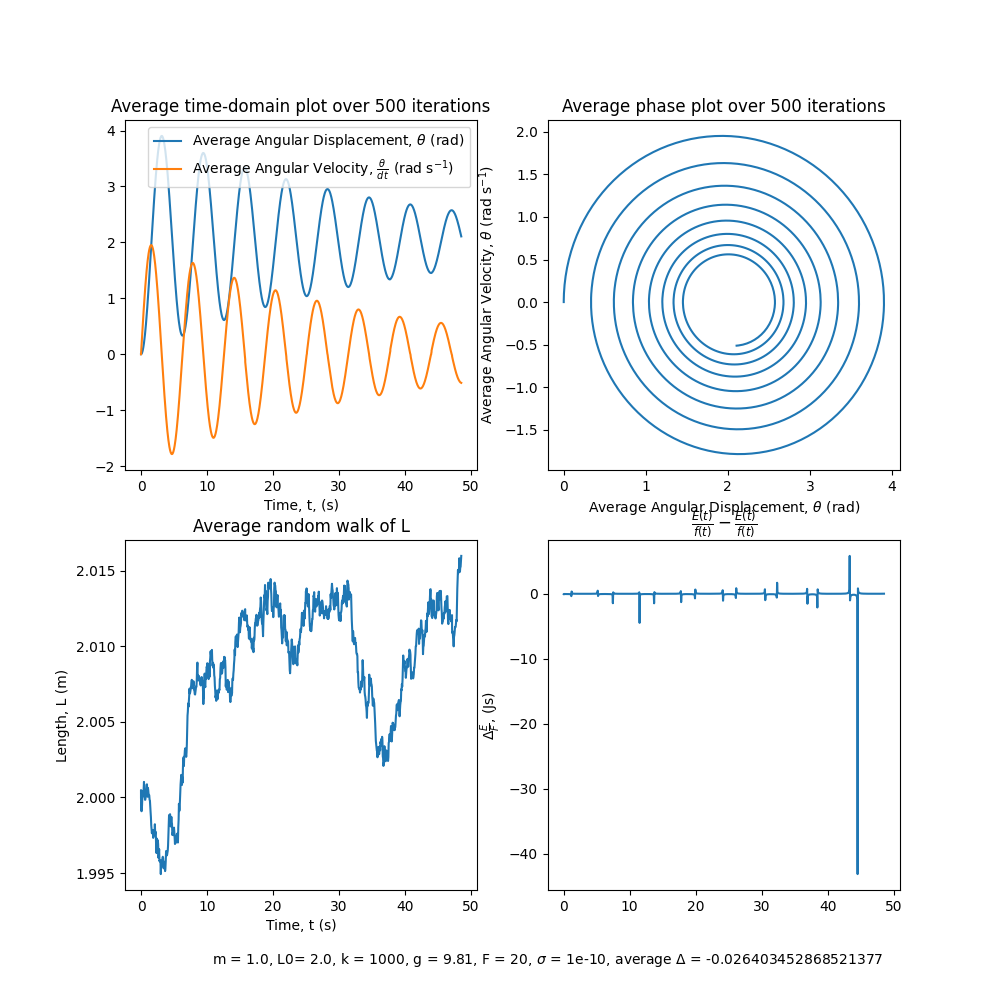
\includegraphics[width = \columnwidth]{Projects/ForcedSimplePendulum/Plots/m = 1.0, L0= 2.0, k = 1000, g = 9.81, F = 20, sigma = 1e-10, run number 8.png}
    \caption{Ninth Iteration.}
    \label{fig:enter-label}
\end{figure}

\begin{figure}
    \centering
    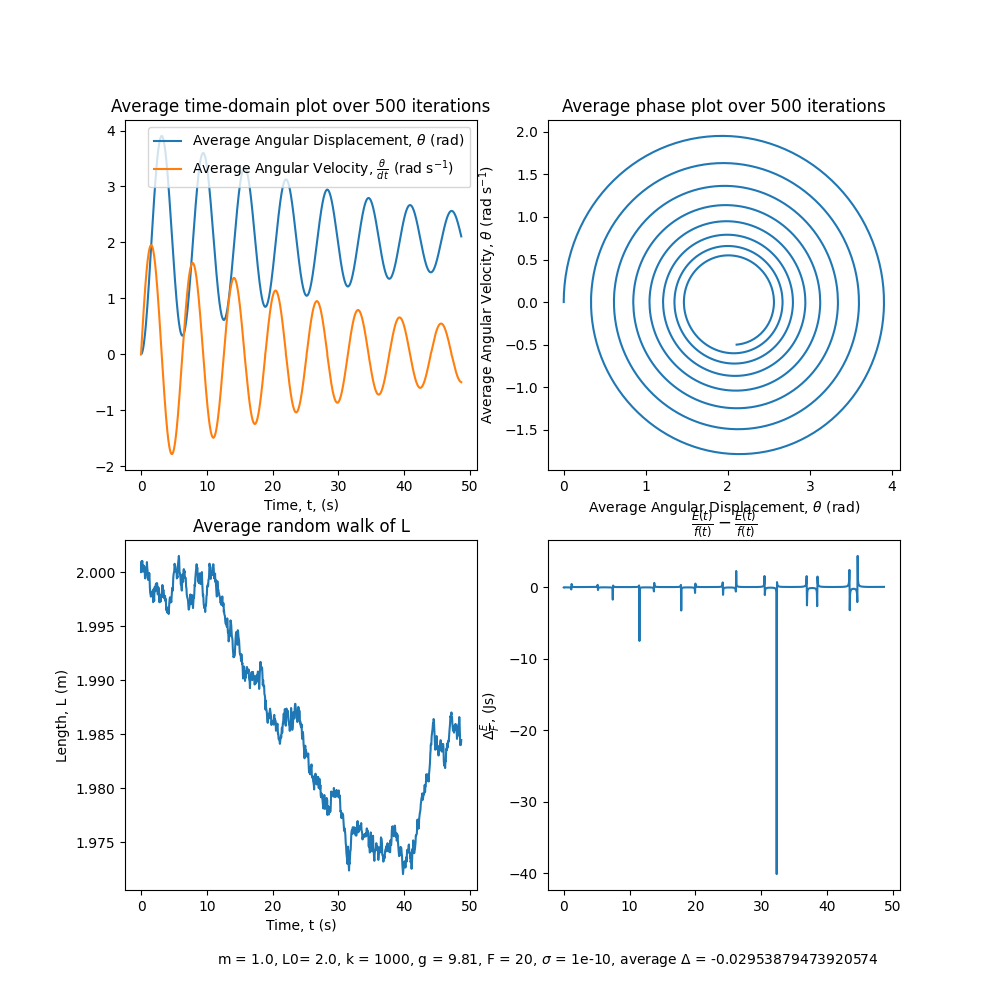
\includegraphics[width = \columnwidth]{Projects/ForcedSimplePendulum/Plots/m = 1.0, L0= 2.0, k = 1000, g = 9.81, F = 20, sigma = 1e-10, run number 9.png}
    \caption{Tenth Iteration.}
    \label{fig:enter-label}
\end{figure}
